% MASTER'S THESIS IN MATHEMATICAL INFORMATION TECHNOLOGY
% Joel Lehtonen and Kristian Siljander
%
% Based on Timo Männikkö's template with some modifications made by
% Tuomo Sipola (M.Sc.).
%
% Uses latex template by Antti-Juhani Kaijanaho and Matthieu Weber.
%

\documentclass[finnish,logo,nonumbib,creativecommons,nocopyright,lof,pdftex,palatino,utf8]{gradu2}

%\usepackage[utf8]{inputenc}

\usepackage{palatino} % Better font
\usepackage[intlimits]{amsmath} % For better math mode, namely integrals
\usepackage{amssymb} % Math symbols

\usepackage[pdftex]{graphicx} % Pictures
\usepackage{pdfpages} % For inclusion of the article

\usepackage{hyperref}
\usepackage{cite}
\usepackage{framed}
\usepackage{verbatim} % Multi-line commenting.
\usepackage{rotating} % Vertical text used in temporary comments.
\usepackage{listings} % Source code


% Optional 1,5 point line spacing
%\usepackage{setspace}
%\onehalfspace

% Kirjastulostusta varten
\usepackage{scalefnt}

% Todo-tags help the examiner's work
\newcommand{\todo}[1]{\marginpar{\begin{framed}\begin{sideways}\textbf{TODO}: #1\end{sideways}\end{framed}}}

% Source code listings. Annotation can be done between [ and ] in Bash.
\lstset{frame=single,captionpos=b}
\renewcommand{\lstlistingname}{Listaus}
\lstdefinelanguage{bashshell}{language=bash,moredelim=[is][\itshape]{[[}{]]},morekeywords={mkdir,find,classifier,ls,parameter_analyzer,xargs,apache2data},aboveskip=0.5cm}
\lstdefinelanguage{MyHaskell}{language=Haskell,morekeywords={ByteString,URL,UTCTime}}

% Define our own abbreviations list
\newenvironment{abbrlist}[1]{
  \begin{list}{}{\settowidth{\labelwidth}{\textbf{#1}}
  \setlength{\leftmargin}{\labelwidth}
  \addtolength{\leftmargin}{\labelsep}
  \renewcommand{\makelabel}[1]{\textbf{\hfill##1}}}}%
{\end{list}}

% No spacing with this enumeration
\newenvironment{enumerate_no_space}{
  \begin{enumerate}
  \setlength{\itemsep}{1pt}
  \setlength{\parskip}{0pt}
  \setlength{\parsep}{0pt}}
{\end{enumerate}}

% Remove pagebackref in the final version
% Add "pagebackref=true" to get page numbers where each reference is used
% Link version for internet viewing
%\usepackage[pdftex,colorlinks=true]{hyperref}

% PDF information tags
\pdfinfo{/Title (WWW-palveluihin kohdistuvien hyökkäysten analyysi ja torjunta) /Author (Joel Lehtonen ja Kristian Siljander) /Subject (Mitähän tähän pitäisi kirjoittaa?) /Keywords (tähän avainsana, toinen, jne.)}

%%% Actual content begins here

\title{Web-palveluihin kohdistuvien hyökkäysten analyysi ja torjunta}
\translatedtitle{Analysis of attacks against WWW services, TODO}

\linja{Mobiilijärjestelmät}

\setauthor{Joel}{Lehtonen}
\setauthor{Kristian}{Siljander}
\yhteystiedot{joel.lehtonen@iki.fi}
\yhteystiedot{kristian.siljander@jyu.fi}
%\setdate{30}{8}{2008}
\license{Tämän teoksen käyttöoikeutta koskee Creative Commons
  Attribution-ShareAlike 3.0 Unported -lisenssi.}

\abstract{ Tahan englanninkielinen tiivistelma }
\tiivistelma{ Tahan suomenkielinen tiivistelma }

\avainsanat{tietoturva, web-palvelut, IDS-järjestelmät}
\keywords{ Web security, IDS-systems}

\begin{document}

% Kirjastulostusta varten fontti luettavamman kokoiseksi
%\scalefont{1.18}

% -*- mode: LaTeX; coding: utf-8; -*-

\termlist

\begin{abbrlist}{ANOVA}
\item[AJAX]	Asynchronous JavaScript And XML. Joukko Web-sovelluskehityksessä käytettyjä tekniikoita.
\item[ARP]	Address Resolution Protocol. Ethernet-verkoissa käytettävä protokolla, jolla selvitetään IP-osoitetta vastaava MAC-osoite.
\item[CSRF]	Cross Site Request Forgery. Web-sovelluksissa esiintyvä tietoturva-aukko, joka väärinkäyttää selaimen ja sivuston välistä luottamussuhdetta.
\item[CSV]	Comma-Separated Values. Tiedostomuoto, jolla tallennetaan yksinkertaista taulukkodataa.
\item[DDoS]	Distributed Denial of Service. Hajautettu palvelunestohyökkäys, jossa hyökkäys tapahtuu samanaikaisesti useasta eri kohteesta.
\item[DOM]	Document Object Model. Ohjelmointirajapinta, joka mahdollistaa HTML- ja XHTML-dokumenttien sisällön muokkauksen.
\item[Dos]	Denial of Service. Palvelunestohyökkäys, jolla pyritään lamauttamaan tietty verkkopalvelu.
\item[HTML]	Hypertext Markup Language. Standardoitu kuvauskieli, jolla kuvataan hyperlinkkejä sisältävää tekstiä.
\item[HTTP]     Hypertext Transfer Protocol. Selainten ja Web-palvelimien käyttämä tiedonsiirtoprotokolla.
\item[ICMP]	Internet Control Message Protocol. TCP/IP-pinon kontrolliprotokolla, jolla lähetetään nopeasti viestejä koneelta toiselle.
\item[IDS]	Intrusion Detection System. Järjestelmä, joka on ohjelmoitu tunnistamaan verkkoon suuntautuvat hyökkäysyritykset.
\item[IIS]      Internet Information Services. Microsoftin kehittämä Web-palvelinalusta.
\item[IPS]	Intrusion Prevention System. Järjestelmä, jolla pyritään ennakoivasti estämään tietomurtoyritykset.
\item[IP]	Internet Protocol. Verkkokerroksen protokolla, joka huolehtii tietoliikennepakettien välittämisestä pakettikytkentäisessä Internet-verkossa.
\item[IRC]	Internet Relay Chat. Pikaviestintäpalvelu, joka mahdollistaa reaaliaikaisen keskustelun Internet-käyttäjien välillä.
\item[JSON]	JavaScript Object Notation. JavaScript-ohjelmissa käytetty yksinkertainen tiedonsiirtomuoto.
\item[LDAP]	Lightweight Directory Access Protocol. Hakemistopalveluiden käyttöön tarkoitettu verkkoprotokolla.
\item[MAC]	Media Access Control. Ethernet-verkossa verkkosovittimen yksilöivä osoite.
\item[OSI]	Open Systems Interconnection Reference Model. Eri tiedonsiirtoprotokollista muodostuva kuvaus.
\item[R2L]	Remote-to-Local. Hyökkäystyyppi, jossa hyökkääjä pyrkii saamaan koneelle laajemmat käyttöoikeudet, kuin hänellä muuten olisi.
\item[SOA]	Service Oriented Architecture. Joustava arkkitehtuuriratkaisu, jolla pyritään helpottamaan eri palveluiden välistä kommunikointia.
\item[SQL]	Structured Query Language. Standardoitu kyselykieli, jolla relaatiotietokantaan voi tehdä hakuja, muutoksia ja lisäyksiä.
\item[TCP]	Transmission Control Protocol. Kuljetuskerroksen protokolla, joka rakentuu IP-protokollan päälle. TCP:tä käytetään lukuisissa sovelluskerroksen protokollissa, esimerkiksi HTTP:ssä.
\item[U2R]	User-to-Root. Hyökkäys, jossa hyökkääjä pyrkii hankkimaan koneelle pääkäyttäjän oikeudet.
\item[UDP]	User Datagram Protocol. Yhteyskäytäntö, jolla sovellus voi lähettää viestejä toiselle tietokoneelle.
\item[VPN]	Virtual Private Network. Menetelmä, jolla useampi verkko voidaan yhdistää näennäisesti samaan yksityiseen verkkoon käyttäen julkista verkkoa. 
\item[XHR]	XMLHttpRequest. Ohjelmointirajapinta, jota käytetään esimerkiksi Ja\-va\-Scrip\-tis\-sä.
\item[XHTML]    eXtensible Hypertext Markup Language. HTML:stä kehitetty kuvauskieli, joka täyttää XML:n muotovaatimukset.
\item[XML]	eXtensible Markup Language. Merkintäkieli, jota käytetään sekä formaattina tiedonvälitykseen järjestelmien välillä että dokumenttien tallentamiseen.
\item[XSS]	Cross Site Scripting. Web-sovelluksissa esiintyvä tietoturva-aukko, joka mahdollistaa käyttäjän koodin syöttämisen sovellukselle.  
\item[Xpath]    XML Path Language. XML-dokumenttien osien osoittamiseen tarkoitettu kieli.	
\end{abbrlist}


\mainmatter

% -*- mode: LaTeX; coding: utf-8; -*-

\chapter{Johdanto}

Viime vuosina Web-sovellusten ja -palveluiden suosio ja käyttö ovat
olleet kovassa kasvussa, ja monet näistä ovat nykyisin kriittisiä osia
yhteiskuntamme toimivuuden kannalta. Internetin välityksellä
käytettävien palveluiden tietoturvan ja saatavuuden takaaminen on
tämän johdosta noussut monessa yrityksessä tärkeään rooliin.
Tietojärjestelmien siirtyminen julkishallinnon ja
yritysten erillisverkoista julkiseen Internetiin on vaikuttanut omalta
osaltaan myös siihen, mihin tietoturvahyökkäykset nykyisin
kohdistuvat ja kuinka ne pyritään toteuttamaan.

Hyökkäysten muuttuessa yhä hienostuneimmiksi, eivät perinteiset
tietoturvamenetelmät enää riitä suojaamaan loppukäyttäjiä tai palvelun
ylläpitäjiä. Tästä syystä erilaisten tietoturvaratkaisuiden ympärillä
käy kova kuhina, ja aihepiiri on herättänyt suurta kiinnostusta
tutkijoiden keskuudessa. Erilaisia ratkaisuja, joissa on pyritty
selvittämään tietoturvahyökkäyksiä ja näiden mukana tulevia haasteita,
on lukematon määrä. Haaste on löytää ne menetelmät, jotka oikeasti
toimivat riittävällä tarkkuudella ja nopeudella.

Tietoturvahyökkäysten tunnistaminen perustuu siihen, että
analysoimalla yhtä tai useampaa tapahtumaa pyritään löytämään
viitteitä tapahtuvista hyökkäyksistä. Menetelmät jaetaan kahteen eri
tyyppiin: anomalioiden eli poikkeavuuksien tunnistamiseen
(engl. \textit{anomaly detection}) ja väärinkäytösten tunnistamiseen
(engl. \textit{misuse detection}). Näistä anomalioiden tunnistaminen
perustuu malleihin, joita luodaan järjestelmän, käyttäjän tai verkon
normaalista käyttäytymisestä. Tulevaa liikennettä sitten verrataan 
näin luotuihin malleihin, jolloin opituista malleista poikkeava liikenne
voidaan tunnistaa. Väärinkäytösten tunnistamiseen tarkoitetut järjestelmät 
puolestaan sisältävät joukon kuvauksia eli signatuureja tunnetuista hyökkäyksistä. 
Tuleva liikenne tarkistetaan näitä kuvauksia vastaan, jolloin näitä vastaavat
hyökkäykset tunnistetaan. Hyökkäysten tunnistusjärjestelmät
jaetaan joissakin tapauksissa myös sen mukaan, mistä tutkittava
liikenne on kerätty. Tällöin järjestelmät on jaettu verkkoon
pohjautuviksi (engl. \textit{network based}) ja asiakaspohjaisiksi
(engl. \textit{host based}).

Tässä tutkielmassa tietoturvahyökkäykset pyritään tunnistamaan analysoimalla 
Web-palvelimien tuottamaa tapahtumalokia. Lokista yritetään etsiä ja tunnistaa
poikkeavuuksia normaalin liikenteen joukosta käyttäen diffuusiokuvauksia. Näiden
avulla pystytään helpommin esittämään ja kuvaamaan sellaista materiaalia, joka 
koostuu suuresta määrästä parametreja.

Tutkielman rakenne on seuraavanlainen. Luvussa 2 esitellään yleisellä
tasolla Web-palvelinalustoja, ja käydään läpi Web-palveluiden
erilaisia toteutustapoja. Luku 3 käsittelee perinteisiä
tietoturvahyökkäyksiä, ja luvussa 4 perehdytään uudenlaisiin
Web-ratkaisuihin ja tietoturvahyökkäyksiin, joiden kohteeksi
Web-palvelut nykyisin joutuvat.  Luku 5 sisältää kuvauksen
dynaamisista Web-teknologioista, jotka mahdollistavat suurimman osan
nykyisistä tietoturvahyökkäyksistä, ja luku 6 sisältää katsauksen
tutkimuskenttään liittyvään tutkimukseen.

Luvussa 7 kuvaillaan analyysissa käytetyt menetelmät, ja luvussa 8
esitellään tutkimuksen lähtökohta ja analysoitavan materiaalin rakenne.
Samassa luvussa myös käydään läpi esikäsittelijää,joka on on suunniteltu 
ja toteutettu tätä tutkimusta varten. Esimerkkien avulla esitellään myös 
sovelluksen toimintaa.

Luvussa 9 esitellään saatuja tuloksia kuvaajien avulla, ja
analyisoidaan näitä tarkemmin sekä esitetään mahdollisia syitä
saatuihin tuloksiin. Jatkotutkimuksia ajatellen esitetään
myös parannusehdotuksia. Viimeinen luku sitten sisältää
yhteenvedon koko työstä ja ajatuksia sen onnistumisesta.

% -*- mode: LaTeX; coding: utf-8; -*-

\chapter{Web-palvelut}

Web-palveluilla tarkoitetaan järjestelmiä, jotka kommunikoivat
keskenään käyttäen vakiintuneita Web-tekniikoita. Web-palvelimet eivät
ole riippuvaisia mistään tietystä laitteisto- tai
käyttöjärjestelmäarkkitehtuurista. Web-palveluiden käyttämät
teknologiat eivät sinänsä ole erityisen vallankumouksellisia, mutta
tiedonvaihdon helpottuminen standardien protokollien ja Web:n
hajautetun rakenteen ansiosta on tehnyt Web-palveluista
mielenkiintoisia niin kehittäjien kuin käyttäjienkin
näkökulmasta\cite{javaweb}.

IBM määrittelee WWW-palvelut seuraavasti: ``Web-palvelut ovat
itsenäisiä ja modulaarisia sovelluksia, jotka voidaan julkistaa,
määritellä, paikallistaa ja suorittaa verkon ylitse, yleeensä WWW:n
välityksellä.''\cite[s.4]{websecurity}

Tietoturvan kannalta WWW-palvelut ovat haastavia, koska niitä
käytetään Internetin välityksellä eivätkä ne ole rajoittuneita
esimerkiksi tietyn organisaation lähiverkkoon. Myös osia
WWW-palveluista sijaitsee usein fyysisesti eri paikoissa ja ne
kommunikoivat keskenään Internetin välityksellä.

Tässa luvussa käsitellään komponentteja, joista tämänhetkiset
Web-palvelut koostuvat. Erityistä huomiota on kiinnitetty seikkoihin,
jotka vaikuttavat palvelun tietoturvaan.

\section{Palvelinohjelmistot}

Web-palveluiden toteuttajan näkökulmasta lähin komponentti on
palvelinohjelmisto. Se käsittelee HTTP-kyselyt ja lähettää vastauksina
käyttäjän selaimessa näytettäviä ja prosessoitavia osia, kuten
hypertekstiä, kuvia ja komentosarjoja.

Web-palvelinohjelmisto ei useinkaan kommunikoi suoraan palvelun
käyttäjän tietokoneen kanssa vaan välissä on usein välimuistipalvelu,
joka vähentää palvelimelle kohdistuvaa rasistusta säilyttämällä
harvoin muuttuvaa sisältöä välimuistissa ja välittämällä tätä suoraan
käyttäjille. Muuttuva tai välimuistille uusi sisältö pyydetään
palvelinohjelmistolta.

Internet-tietoturvapalveluita tarjoavan Netcraftin\cite{netcraft}
raportista huhtikuulta 2010 käy ilmi, että kaksi suurinta
Web-palvelinalustaa ovat Apache (53.93\% suosituimmista sivuista),
Microsoft (24.97\%). Näiden jälkeen tulevat Google ja nginx kumpikin 6\%
osuudella.

Tuloksia voi vääristää jonkin verran se, että joissakin tapauksissa
edustalla suoritetaan välimuistipalveluna toista palvelinohjelmistoa,
esimerkiksi Apachea tai nginx:ä, joka välittää kyselyt eteenpäin
varsinaiselle Web-palvelinohjelmistolle. Tämä selittää esimerkiksi
sen, miksi Zope puuttuu kokonaan suosituimpien palvelinten
joukosta. Esimerkiksi Jyväskylän yliopiston Web-palvelimena näkyy
tilastoinnissa Apache, vaikka Web-palvelu on toteutettu
Zope-palvelinohjelmiston päällä suoritettavalla Plonella. Samoin on
käynyt Tomcat-palvelimella ajettavalle Korppi-opintotietojärjestelmälle.

\subsection{Apache}

Suosituimpana palvelinalustana Apache on luonnollisesti suosittu kohde
myös tietomurtojen yrityksille. Apachesta itsestään on kuitenkin
löydetty verrattain vähän
tietoturva-aukkoja.~\cite{apachetietoturva}. Suurin osa tietomurroista
keskittyykin murtamaan varsinaista Web-palvelua palvelinalustan sijaan.

Apache pystyy suorittamaan komentosarjoja perinteisen CGI-rajapinnan
lisäksi myös palvelinlaajennosten avulla, jolloin saavutetaan
tiiviimpi integraatio ja enemmän suorituskykyä verrattuna
CGI-rajapintaan~\cite{cginopeus}.

Apachea voidaan suorittaa lukuisissa eri käyttöjärjestelmissä, joista
Linux on ylesiin~\cite{apachemarket}. Suosittuja Apache-alustalla
käytettäviä ohjelmointikieliä ovat PHP ja Python. Tunnettuja tässä
ympäristössä käytettäviä Web-palveluita ovat mm. Wikipediassa
käytettävä MediaWiki ja lukuisilla selainkäyttöisillä
keskustelupalstoilla käytettävä phpBB.

TODO LAMP (Linux + Apache + MySQL + PHP)

\subsection{Zope}

+Plone. TODO

\subsection{Tomcat}

TODO

\subsection{IIS}

TODO.

\section{Hajautetut palvelut}

TODO Pyynnön ohjaaminen usealle palvelimelle (reverse proxy), Hyödyt verrattuna keskitettyyn

\section{Välimuistipalvelut}

TODO 
- "talon sisällä" olevat välimuistit
 - Akamai ym. "ulkoiset" välimuistit (ei luovuta esim. IP-osoitteita)
 - tiedon keräämisen kannalta IDS:lle (minkälaiset logitukset?)


% -*- mode: LaTeX; coding: utf-8; -*-

\chapter{Perinteiset tietoturvahyökkäykset}

Tietoyhteiskunnassa yksikään verkossa oleva laite ei ole suojassa
tietoturvahyökkäyksiltä, ja niiden mukanaan tuomilta
ongelmilta. Hyökkäykset ovat nykyisin myös hyvin monimuotoisia ja ne
voidaan jakaa eri kategorioihin niiden tavoitteiden ja toteutustapojen
mukaan. Uusia hyökkäystapoja kehitetään jatkuvasti lisää ja
tunnetutkin hyökkäystavat saavat uusia ominaisuuksia. Vaikka
suurimpaan osaan hyökkäyksistä on olemassa erilaisia
suojautumistapoja, on näiltä kaikilta suojautuminen ylläpitäjän
kannalta mahdoton tehtävä. Verkon turvallisuuden kannalta on kuitenkin
tärkeää, että hyökkäysten riskit tiedostetaan ja uhkien toteutumisen
todennäköisyyksiä voidaan pienentää mahdollisuuksien ja resurssien
rajoissa.


\section{Tiedon urkinta ja väärentäminen}

Ennen kuin hyökkääjä pystyy murtautumaan verkkoon tai verkossa
sijaitsevaan tietokoneeseen, tulee hänen selvittää järjestelmän
mahdolliset heikkoudet. Haluttuja tietoja ovat esimerkiksi asennetut
käyttöjärjestelmät, ohjelmistojen versiotiedot sekä verkon yleinen
rakenne ja tietoturvataso. Näiden tietojen selvittämiseksi hyökkääjä
aloittaa verkkoa kohtaan joukon hyökkäyksiä, joita kutsutaan
tiedusteluhyökkäyksiksi (engl. \textit{Probe Attacks}). Tällaiset
tiedustelut ovat varsinaisia hyökkäyksiä yleisempiä, sillä niiden
toteuttaminen ei vaadi hyökkääjältä kovin syvällistä
osaamista. Verkosta löytyy paljon valmiita työkaluja, joiden avulla
hyökkääjä pystyy urkkimaan tarvittavat tiedot ja mahdollisesti jo
saman tien hyödyntämään havaittuja heikkouksia. Hyökkääjä, jolla on
tietämystä verkossa käytettävistä laitteista ja palveluista, voi
hyödyntää näitä tietoja haavoittuvuuksien etsimiseen ja järjestelmien
murtautumiseen \cite{IDS}.

Kun hyökkääjällä on riittävä tietämys verkon eri komponenteista, voi
hän aloittaa hyökkäyksen suunnittelun. Yksi tapa murtautua
tietoverkkoon on hyödyntää verkkokerroksen protokollissa, kuten TCP ja
IP, olevia heikkouksia. Tällaisia hyökkäyksiä kutsutaan
\textit{spoofing}- eli \textit{petkutushyökkäyksiksi}. Niissä
murtautuja pyrkii naamioimaan oman koneensa siten, että se näyttäa
kuuluvan kohteena olevan laitteen kanssa samaan lähiverkkoon.  Tällöin
hyökkääjä pystyy helpommin huijaamaan kohdekonetta jakamaan ja
lähettämään arkaluontoista tietoa, jota jaettaisiin muuten ainoastaan
luotettujen osapuolien kesken.  Tällaiset hyökkäykset jaotellaan
edelleen sokeisiin ja aktiivisiin hyökkäyksiin sen mukaan, kuinka
paljon hyökkääjällä on tietoa verkon rakenteesta. Sokeassa
hyökkäyksessä kohdekoneen lähettämiä vastauksia ei pystytä seuraamaan,
koska murtautujan oikeudet ovat puutteellisia ja IP-osoite, jonka
haltijaksi hyökkääjä haluaa naamioitua, on harvoin tiedossa.
Aktiivisessa hyökkäyksessä murtautujalla on käytettävissään tietoa
tietokoneiden välisistä käyttöoikeuksista, jolloin tiedon
korruptoiminen, muokkaaminen ja välittäminen toiseen verkkoon on
helpompaa toteuttaa \cite{WEBS}.

\subsection{IP Spoofing}

IP Spoofing on hyökkäys, jossa pyritään murtautumaan verkkoon ja
hankkimaan arkaluontoista tietoa väärentämällä lähetettäviin
paketteihin luotetun koneen IP-osoite. Hyökkäykset jaotellaan
sokeisiin ja aktiivisiin hyökkäyksiin sen mukaan, mistä hyökkäys
toteutetaan. Hyökkäykset toimivat siten, että kolmivaiheisen
yhteydenmuodostuksen aikana hyökkääjä tekeytyy tietokoneeksi, johon
hyökkäyksen kohteella on luottamussuhde. Tämä tapahtuu muokkaamalla
lähetettävien pakettien otsaketietoja ja kuittausnumeroita. Tässä
onnistuakseen hyökkääjän tulee pystyä vastaamaan oikeilla
kuittausnumeroilla kohteen lähettämiin paketteihin. Nämä
kuittausnumerot hyökkääjä joutuu aluksi usein arvaamaan, jonka vuoksi
tämä hyökkäystapa on vaikea toteuttaa \cite{WEBS}. Niin kutsuttu Man
in The Middle -hyökkäys, jossa hyökkääjä kaappaa kahden koneen välisen
yhteyden, perustuu myös IP-\-osoitteen väärinkäyttöön. Kuva \ref{Man}
havainnollistaa hyökkäyksen toteuttamista.

\begin{figure}[ht]
\centering
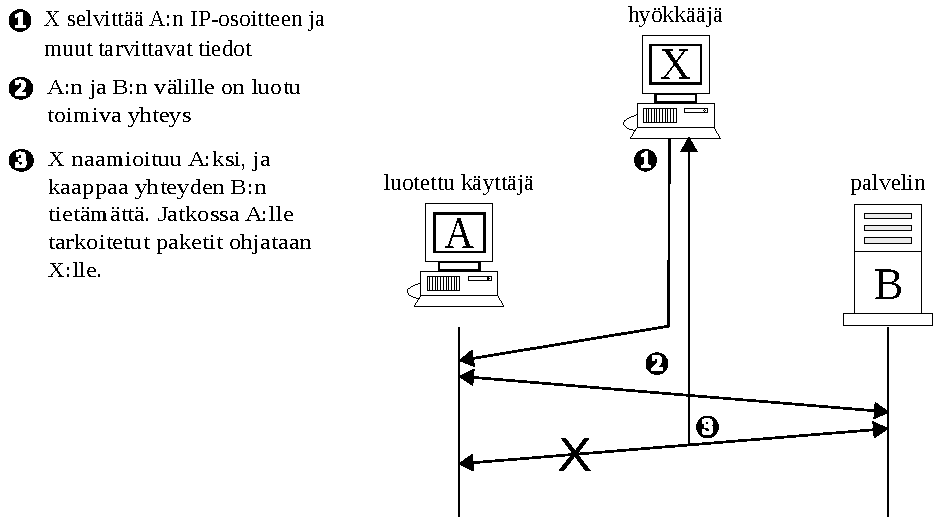
\includegraphics[width=13cm]{pics/MiTM.pdf}
\caption{Man in The Middle-hyökkäys}
\label{Man}
\end{figure}

Vaikka IP-osoitteen väärentämiseen perustuvat hyökkäykset ovat
vaikeita toteuttaa, ovat ne melko yleisiä, sillä jokainen
TCP/IP-protokollaa käyttävä järjestelmä on niille alttiina. Tämä
johtuu siitä, että TCP/IP-verkossa on sallittua muokata paketteja
tiedonsiirron aikana. Näin on, koska eräät IP-pohjaiset palvelut
edellyttävät pakettien sisällön muuttamista lähettämisen
yhteydessä. Tällaisia palveluita ovat esimerkiksi mobiili-IP- ja
VPN-järjestelmät.~\cite{DDOS}.

IP spoofing -hyökkäyksiä voidaan torjua monin eri keinoin. Tehokkain
tapa on määritellä verkon reitittimet estämään sellaisten pakettien
kulku, jotka on merkitty lähetetyiksi sisäverkon laittelta, mutta
jotka todellisuudessa saapuvat reitittimeen sen ulkopuolisista
liitännöistä. Jos tämä kuitenkin halutaan sallia, niin jokainen sessio
tulisi kryptata reitittimessä. Muutenkin yhteyksien muodostumisen
tulisi pohjautua koko järjestelmän kattavaan salaukseen \cite{WEBS}.

% TODO: tarkista, mitä tällä kryptaamisella reitittimessä oikein
% tarkoitetaan.

\subsection{ARP Spoofing}

Nykyisin lähes jokainen verkko pohjautuu TCP/IP-protokollan ja
Ethernet-verkon väliseen yhteistoimintaan. Tässä yhteydessä tarvitaan
ARP-pro\-to\-kol\-laa, jonka tehtävänä on selvittää IP-osoitteita
vastaavat Ethernet- eli MAC-osoiteet. Ethernet-osoite
verkkokorttikohtainen ja sen avulla yksilöidään lähiverkossa
sijaitsevat tietokoneet ja muut aktiivilaitteet.  Tietoa tarvitaan
myös IP-protokollalla liikennöitäessä, koska ilman tietoa
Ethernet-osoitteesta lähiverkossa sijaitseva reititin ei pystyisi
välittämään Internetistä saapuvia paketteja eteenpäin oikealle
laitteelle eikä myöskään lähiverkossa sijaitseva tietokone pystyisi
siirtämään tietoa IP-protokollalla muille lähiverkossa sijaitseville
laitteille.

ARP spoofing -hyökkäyksessä, jota kutsutaan myös ARP-myrkyttämiseksi,
pyritään syöttämään syöttämään reitittimien ARP-tauluihin virheellistä
tietoa (kuva \ref{ARP-spoofing}). Tämä tapahtuu kaappaamalla verkon
yleislähetysviestejä ja muokkaamalla kuittausviestien sisältöä siten,
että kuittausviesteihin hyökkääjä laittaa kohdeosoitteeksi oman
IP-osoitteensa. Verkon aktiivilaitteilta saapuviin, muille
tarkoitettuihin kyselyihin vastataan omalla MAC-osoitteella.  Tämän
jälkeen kohdelaitteelle tarkoitetut paketit ohjautuvatkin hyökkääjän
koneelle \cite{WEBS}.

ARP-protokolla on hyvin haavoittuvainen hyökkäyksille, koska
oletuksena se ei sisällä minkäänlaista suojautumiskeinoa
ARP-myrkyttämiselle. Siksi paras keino suojautua tällaisilta
hyökkäyksiltä on varmistaa, että ennen ARP-taulun muokkausta
tunnistetaan käyttäjät jollakin keinolla. Toinen mahdollisuus on
käyttää verkkolaitteissa staattisia ARP-tauluja~\cite{WEBS}. Jakamalla
lähiverkko pienempiin osiin virtuaalisten lähiverkkojen (VLAN) avulla
voidaan myöskin rajata ARP-myrkyttämisen vaikutuksia.

\begin{figure}[ht]
\centering
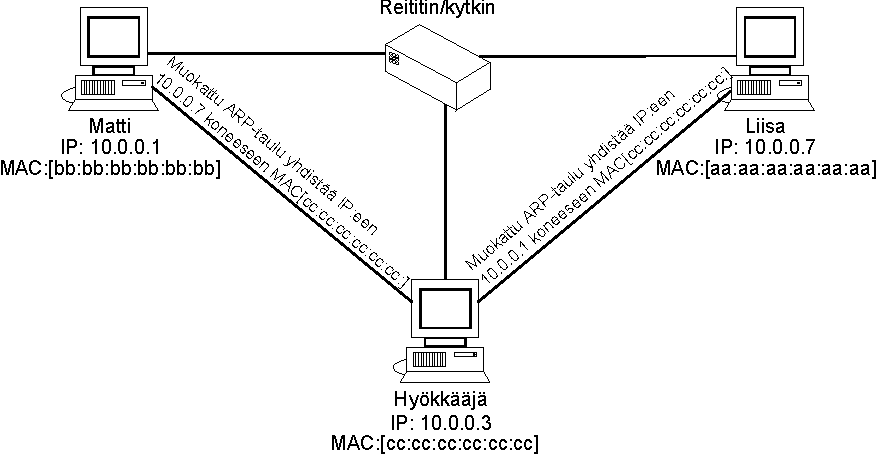
\includegraphics[width=12cm]{pics/arp.pdf}
\caption{ARP-taulun myrkyttäminen käyttäen Man In the Middle -hyökkäystä.}
\label{ARP-spoofing}
\end{figure}

\section{Denial Of Service}

CERT \cite{CERT}, joka on yksi tietoturva-alan johtavista
tutkimuskeskuksista, määrittelee palvelunestohyökkäyksen
(engl. \textit{Denial of Service}, DoS) sellaiseksi teoksi, jossa
hyökkääjän tavoitteena on estää palvelun käyttäjiä käyttämästä heille
kuuluvia tai heidän käytettävissään olevia palveluita. Tällaisia
palveluita voivat olla esimerkiksi tietoliikenneresurssit tai verkossa
käytettävät Web-sovellukset. Hyökkäyksillä pyritään lamauttamaan
palvelua tarjoava verkko tai palvelin siten, että asiaankuuluvien
pyyntöjen vastaanottamiseen tai käsittelyyn ei enää riitä
resursseja. Keinoja hyökkäysten toteuttamiseen on monia. Koska
valtaosa palvelunestohyökkäyksistä käyttää hyväkseen eri protokollien
sallittuja toimintoja, on hyökkäyksiltä suojautuminen hyvin vaikeaa
\cite{Hacking}.

Palvelunestohyökkäykset voidaan jakaa kolmeen ryhmään näiden
toteutustapojen ja tavoitteiden mukaan. Ensimmäiseen ryhmään kuuluvat
hyökkäykset, joiden tarkoituksena on kuormittaa palvelimia ja kuluttaa
loppuun niiden rajoitetut resurssit. Tämä voidaan toteuttaa esimerkiksi
kuormittamalla verkkoa tai palvelinta turhilla pyynnöillä. Toiseen
ryhmään kuuluvat hyökkäykset, jotka pyrkivät joko tuhoamaan tai
muuttamaan konfigurointitietoja siten, että kone tai verkko lakkaa
toimimasta. Viimeiseen ryhmään kuuluvat verkon komponenttien
muokkaamiseen tai tuhoamiseen tähtäävät hyökkäykset
\cite{CERT}. Vaikka tässä työssä keskitytään vain resursseihin
kohdistuviin hyökkäyksiin, niin palvelun kokonaisturvallisuuden
kannalta ylläpitäjän tulee kiinnittää jokaiseen ryhmään tasapuolisesti
huomiota.

% TODO näistä kolmesta voisi tehdä söpön taulukon.

Viime vuosina palvelunestohyökkäysten kirjo on voimakkaasti
laajentunut. Alkuperäisten, pelkästään verkkokerroksen raa’an voiman
hyökkäysten, lisäksi on alkanut esiintyä sovelluskerroksen
hyökkäyksiä, joiden toteuttaminen vaatii hyökkääjältä usein varsin
vähän omia resursseja \cite{Hacking}. Nämä sovelluskerroksen
hyökkäykset ovat toteutukseltaan hyvin hienostuneita, jolloin ne
jäävät yleensä huomaamatta tavanomaisilta tietoturvajärjestelmiltä,
koska tietoliikenteen sisältö ei juurikaan poikkea
normaalitilanteesta. Hyökkääjä saattaa esimerkiksi pyytää sellaista
resurssia palvelulta, jonka kysely vie vain vähän hyökkääjän omia
resursseja, mutta aiheuttaa palvelimelle suuren kuormituksen
\cite{DDOSb}.

Sovelluskerroksen hyökkäysten teho nähtiin vuonna 2004, kun
MyDoom-\-viruksella saastuneet koneet kuormittivat yleisimpiä
hakukoneita etsimällä näiden avulla uusia sähköpostiosoitteita, joihin
lähettää saastunut sähköposti \cite{Hacking}. Sovelluskerroksen
hyökkäyksen vaikutus voidaan kohdistaa myös yksittäisiä palveluita
kohti, jolloin vaikutukset ovat vieläkin suuremmat. Näin tapahtui
vuonna 2003, kun Yhdysvalloissa yrittäjä palkkasi ns. DDoS-mafian
kaatamaan kilpailijoidensa verkkosivut HTTP-kyselyillä, jotka pyysivät
ladattavaksi isoa kuvatiedostoa \cite{DDOSb}. Tämä aiheutti kolmelle
kilpailijalle arviolta jopa miljoonan dollarin tappiot ja pysäytti
näiden liiketoiminnan lähes kahdeksi viikoksi \cite{FBI}.

\subsection{SYN-hukuttaminen}
TCP/IP-protokollan yksi suunnittelulähtökodista oli, että sitä
käytettäisiin avoimessa ja luotetussa ympäristössä. Tästä syystä sen
suunnittelussa ei osattu ottaa huomioon mahdollisia vihamielisiä
käyttäjiä, jotka pyrkisivät häiritsemään muiden käyttäjien
tietoliikennettä. TCP/IP-protokollan käyttö julkisissa verkoissa kuitenkin
yleistyi arvaamattomasti, jonka vuoksi suunnitteluvaiheessa tehdyt
virheet periytyivät nyt käytössä olevaan IPv4-verkkojen rakenteisiin
\cite{Hacking}.

Yhteydenmuodostus TCP-protokolla tapahtuu kolmivaiheisesti. Aluksi
yhdistävä tietokone lähettää palvelimelle SYN-paketin, jonka
seurauksana palvelin varaa tulevalle yhteydelle resursseja ja lähettää
yhdistävälle tietokoneelle SYN/ACK-paketin. Tämän jälkeen palvelin
jää odottamaan yhteyden muodostamista. Tähän yhdistävän tietokoneen
tulee vastata ACK-paketilla, jonka jälkeen yhteys on muodostunut ja
tiedonsiirto voi alkaa \cite{Hacking}. Tunnetuin TCP:tä käyttävä
protokolla on Webissä käytettävä HTTP. Sen avulla Web-palvelimet
pystyvät nopeasti palvelemaan useita yhtäaikaisia käyttäjiä.

TCP/IP-protokollan historiasta perityistä heikkouksista tunnetuin ja
käytetyin on SYN-hukuttamiseksi kutsuttu hyökkäys, jossa hyökkääjä
pyrkii kuluttamaan kohteen tietoliikennekapasiteetin loppuun
tekaistuilla yhteydenmuodostuspyynnöillä. Hyökkäys on hyvin
yksinkertainen ja helppo toteuttaa, sillä se käyttää hyväkseen
TCP-protokollaan määritettyjä toimintoja. Hyökkäyksessä
TCP-protokollan kolmiosaista yhteydenmuodostusta ei viedä loppuun
saakka vaan jätetään palvelin odottamaan ACK-paketti yhdistävältä
tietokoneelta.

Koska TCP-protokolla pyrkii aina varmistamaan yhteyden muodostumisen,
lähetetään SYN/ACK-paketti tarvittaessa uudestaan, kunnes yhdistävä
tietokone vastaa ACK-paketilla tai määritelty aikaraja tulee
vastaan. Tätä ominaisuutta hyökkääjä pystyy käyttämään
hyväkseen. Riittää, että hyökkääjä nuuskii selville käyttämättömän
IP-osoitteen, joka on vielä mieluiten samasta aliverkosta kuin missä
palvelin sijaitsee. Tämän jälkeen hyökkääjä luo SYN-paketin, jossa on
tämä tekaistu IP-osoite. Koska palvelimen lähettämä SYN/ACK-viesti ei
koskaan saavu oikealla koneelle, ei palvelin saa ACK-kuittausta. Tällöin
TCP-protokolla alkaa lähettämään pakettia uudestaan niin kauan
kunnes määritetty raja yhteyden aikakatkaisulle tulee vastaan
\cite{STACK}. Hyökkääjän on vaivatonta automatisoida nämä vaiheet ja
hyökkäys voidaan toteuttaa esimerkiksi saastuneista koneista
muodostetun verkoston avulla. Näin saadaan aikaiseksi kuvan \ref{syn}
mukainen tilanne, jossa useita IP-osoitteita käyttämällä hyökkääjä
häiritsee kohteen toimintaa turhilla yhteydenottopyynnöillä.

\begin{figure}[hpt]
\centering
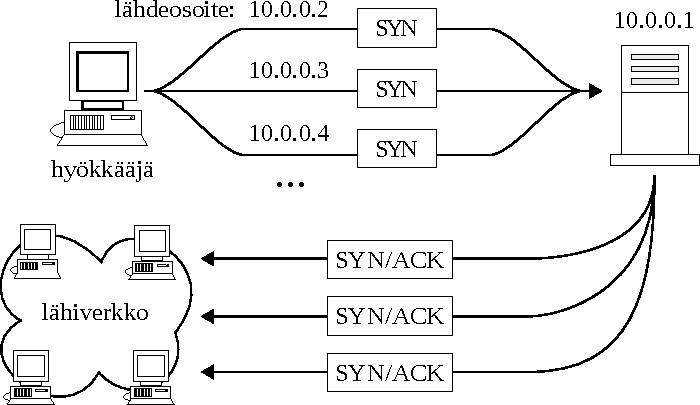
\includegraphics[width=12cm]{pics/syn.pdf}
\caption{SYN-hyökkäys käyttäen useita lähiverkon IP-osoitteita.}
\label{syn}
\end{figure}

SYN-hukuttamisen mahdollistavan mekanismin avulla voidaan myös toteuttaa
heijastettu hyökkäys (engl. \textit{reflective attack}), joka on muunnos 
SYN-hukuttamisesta. Tässä hyökkäyksessä väärennetyissä SYN-viesteissä on
lähettäjäksi merkitty haluttu kohde. Lähettämällä suuri määrä näitä SYN-viestejä 
esimerkiksi Web-\-palvelimelle, aiheutuu vastaustulvasta ongelmia
kohteelle \cite{STACK}.

Koska ylimääräistä palvelinkapasiteettia ei useinkaan ole järkevää
pitää SYN-\-hukuttamisen varalta, joudutaan ratkaisua
hakemaan muualta. Alkeellisin keino on rajoittaa puoliavonaisten
yhteyksien määrää, jolloin rajan ylittyessä yhteyksiä aletaan
pudottamaan \cite{TCP}. Toinen käytetty keino on reitittimiltä
verkkoon päin tulevan liikennemäärän seuraaminen ja liikennepiikkeihin
reagoiminen. Hyökkäyksiä vastaan voidaan myös suojautua liikenteen
seuraamiseen tarkoitetuilla sovelluksilla sekä pääsylistoilla
\cite{STACK}.

Kehittyneempi suojautumiskeino on muuttaa TCP-protokollan kättelyä
siten, että yhteyden tarvitsemat resurssit varataan vasta ACK-viestin
vastaanottamisen yhteydessä. Tätä menetelmää kutsutaan
SYN-evästykseksi (engl. \textit{SYN Cookies}) ja se on tuettu
mm. Linuxissa ja FreeBSD:ssä~\cite{syncookies}. Yhteydenmuodostuksessa
tarvittavat parametrit kätketään tällöin SYN-paketin
järjestysnumeroon. Tämän menetelmän käyttö kuitenkin rajaa pois
runsaasti TCP-protokollan ominaisuuksista, jonka vuoksi SYN-evästys
kytketään yleensä päälle vain hyökkäysten ajaksi.

Täydellistä ratkaisua SYN-hukuttamista vastaan ei mikään näistä
tavoista kuitenkaan tarjoa. Huolellisesti toteutettua hyökkäystä on
vaikea torjua.

\subsection{UDP Echo}

Myös UDP-protokollan käyttö mahdollistaa hyökkäysten tekemisen. Nämä
hyökkäykset käyttävät hyväkseen UDP Echo -protokollaa, mikäli sen
käyttö on sallittu verkossa. Näistä hyökkäyksistä tunnetuin on
Fraggleksi nimetty hyökkäys, joka nykyisinkin aiheuttaa väärin
konfiguroidussa verkossa suuria ongelmia.  Fraggle toimii siten, että
hyökkääjä lähettää UDP Echo -viestin yleislähetyksenä, johon on
merkitty lähettäjäksi hyökkäyksen kohde. Tähän viestiin kaikki verkon
koneet pyrkivät vastaamaan, jolloin kohdetietokoneen
tietoliikennekapasiteetti ja resurssit käytetään viestien
vastaanottamiseen (kuva \ref{fraggle}).

Fraggle on hyvä esimerkki vahvistetusta hyökkäyksestä, jossa verkon
laitteiden määrä vaikuttaa siihen, kuinka vakava hyökkäys on
\cite{WEBS}. Vastaavanlainen hyökkäys voidaan myös toteuttaa kahden
koneen välillä, jos kummassakin on sallittuna UDP Echo
-viestit. Tällöin hyökkääjä väärentää viestiin lähettäjän osoitteen ja
halutun kohdeportin. Vastaanottaja vastaa tähän viestiin omalla
Echo-viestillä, ja näin kahden koneen välille muodostuu ikuinen
silmukka \cite{TCP}.

\begin{figure}[htp]
\centering
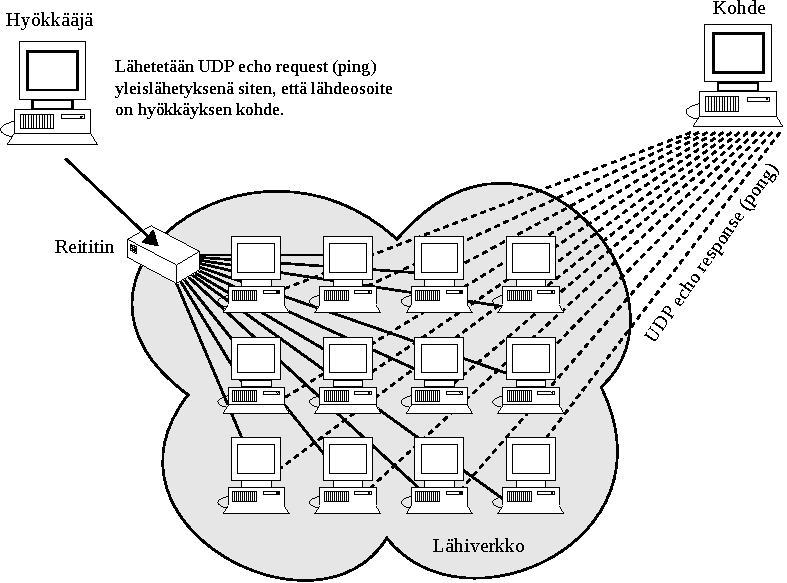
\includegraphics[width=13cm]{pics/fraggle.pdf}
\caption{Vahvistettu UDP Echo -hyökkäys.}
\label{fraggle}
\end{figure}

\subsection{Smurf}

Smurf on yksi ensimmäisistä vahvistetuista DoS-hyökkäyksistä, ja se
toimii lähes identtisesti Fragglen kanssa sillä erolla, että UDP:n
sijasta käytetään ICMP-\-protokollaa. Hyökkääjä lähettää kohteen
puolesta yleislähetyksenä verkolle ICMP Echo -paketin, johon verkon
laitteet vastaavat, jos Echo-viestit on sallittuja verkossa. Jo 100
tietokoneen lähiverkko pystyy aiheuttamaan 14 Mb/s haittaliikenteen
kohdekoneelle, joten pienessäkin väärin konfiguroidussa verkossa
on mahdollista muodostaa riittävästi haittaliikennettä tietoliikenteen
häiritsemiseen tai estämiseen \cite{Hacking}.

Jos hyökkäys on päässyt käyntiin, ei tälle ole paljoa muuta tehtävissä
kuin poistaa kohteena olevat laitteet pois verkosta. Paras vastatoimi
Fragglen ja Smurffin kaltaisille hyökkäyksille on konfiguroida verkon
laitteet alusta asti oikein. ICMP Echo -yleislähetysten estämisellä
pääsee jo pitkälle. ICMP-protokollan käyttöä verkossa kannattaa
muutenkin tarkkailla ja tarvittaessa rajoittaa \cite{Hacking}.

\section{Distributed Denial of Service}

Vielä viime vuosikymmenellä palvelunestohyökkäykset perustuivat
yleensä käyttöjärjestelmistä löydettyjen heikkouksien
hyödyntämiseen. Näiden hyökkäysten aikaansaama tuho riippui paljon
käytettävistä järjestelmistä ja vahingot olivat melko
rajattua. Palvelunestohyökkäyksiä ei nähty tällöin kovinkaan vakavana
uhkana, mutta suhtautuminen muuttui 2000-luvulle tultaessa, kun
hajautetut palvelunestohyökkäykset (engl. \textit{Distributed Denial
of Service}) kehitettiin. Tällaisessa hyökkäyksessä palvelua saattaa
olla lamauttamassa jopa yli 140~000 saastunutta konetta. Tällaisia
saastuneita koneita kutsutaan zombeiksi (engl. \textit{zombie}).

Tietokone voidaan muuttaa zombiksi murtautumalla ja asentamalla siihen
ohjelmisto, jonka avulla murtautuja pystyy hallitsemaan laitetta
käyttäjän tietämättä. Zombiverkoston ei tarvitse edes olla kovinkaan
suuri aiheuttaakseen tuhoa, sillä jo 3~000 koneen verkosto, jossa
jokainen kone tuottaa 25 kb/s liikennettä, aiheuttaa yhteensä 75 Mb/s
kuormituksen verkolle \cite{Hacking}.  Palvelunestohyökkäyksen
seuraamukset ovat varautumattomalle taholle usein katastrofaaliset ja
pahimmillaan hyökkäys saattaa pysäyttää organisaation toiminnan
useiksi päiviksi \cite{CERT}.

Hyökkäysten hajauttaminen useammalla koneelle tuo useita hyötyjä
verrattuna perinteiseen palvelunestohyökkäykseen, jossa hyökkäys
toteutetaan käyttäen yhtä konetta. Otetaan esimerkiksi vaikka
Web-palveluita tarjoava palvelin, jota vastaan halutaan tehdä
palvelunestohyökkäys. Tällaisella palvelimella on käytössä
huomattavasti suurempi määrä resursseja (tietoliikennekapasiteetti,
muisti, laskentateho) kuin yksittäisellä zombitietokoneella on. Kun
hyökkäys suoritetaan yhtäaikaisesti useammalla koneella, pystyy
hyökkääjä kuluttamaan suuretkin resurssit loppuun lyhyessä
ajassa. Yksittäiseltä koneelta tuleva palvelunestohyökkäys on helppo
tunnistaa ja estää verkon ylläpitäjän toimesta. Hyökkääjien määrän
kasvaessa tehtävä vaikeutuu huomattavasti, koska haittaliikennettä
aiheuttavat tietokoneet tai itse haittaliikenne pitää tunnistaa
hyötyliikenteen joukosta. Mikäli zombitietokoneet ovat sijoittuneet ympäri
Internetiä, on hyökkäysten pysäyttäminen ilman palvelun laadun heikkenemistä
mahdoton tehtävä ilman automatisointia. Haittaliikennettä on tällöin myös
vaikea erottaa tavallisesta liikenteestä, koska se tulee palvelimelle
useita reittejä pitkin \cite{DDOS}.

Nopeiden yhteyksien ja verkossa olevien tietokoneiden räjähdysmäinen
kasvu on tehnyt hajautetuista palvelunestohyökkäyksistä hyvin
tehokkaita ja tuhoisia. Suuri määrä verkkoon liitetyistä laitteista on
huonosti suojattu ja päivitetty, ja ihmisten tietoisuus verkon
vaaroista on usein puutteellista. Tämä on luonut otollisen maaperän
suurten zombiverkostojen muodostamiselle virusten ja matojen
avustuksella. Tarjolla on myös tätä tarkoitusta varten suunniteltuja
työkaluja ja ohjelmistoja, jotka tekevät tarvittavat toimenpiteet
automaattisesti. Jo ensimmäiset, vapaasti saatavilla olevat työkalut,
kuten Trinoo ja Shaft, mahdollistivat tuhansien suojaamattomien
koneiden haltuunoton ilman suurempaa perehtymistä \cite{DDOS}.

Hyökkäyksessä käytetyt koneet voidaan jakaa agentteihin (engl. \textit{agents})
ja liikenteen ohjaajiin (engl. \textit{handlers}) riippuen näiden
rooleista. Näistä koneista hyökkääjä käskyttää suoraan liikenteen
ohjaajia, jotka ohjaavat edelleen annetut käskyt agenteille
hyökkäyksen alettua \cite{WEBS}\cite{DDOS}. Ensimmäisissä 
DDoS-verkoissa nämä ohjausviestit olivat salaamattomia, jolloin kuka tahansa
pystyi kaappaamaan näitä. Tämä oli tietomurtojen tekijöiden
näkökulmasta ongelmallista, koska liikenteen ohjaajat joutuivat
ylläpitämään listaa agenttien käyttämistä IP-osoitteista. Mikäli liikenteen välittäjä
joutui vastahyökkäyksen kohteeksi, pystyttiin selvittämään zombiverkon jokaisen
laitteen osoitteet. Tätä suoran käskyttämisen heikkoutta pyrittiin korjaamaan muun
muassa salaamalla käytettävä viestiliikenne. Ajan saatossa liikenteen
ohjaajat pystyttiin kuitenkin tunnistamaan ja poistamaan verkosta,
jolloin hyökkäyksessä käytetty zombiverkko hajosi \cite{DDOS}.

\begin{figure}[htp]
\centering
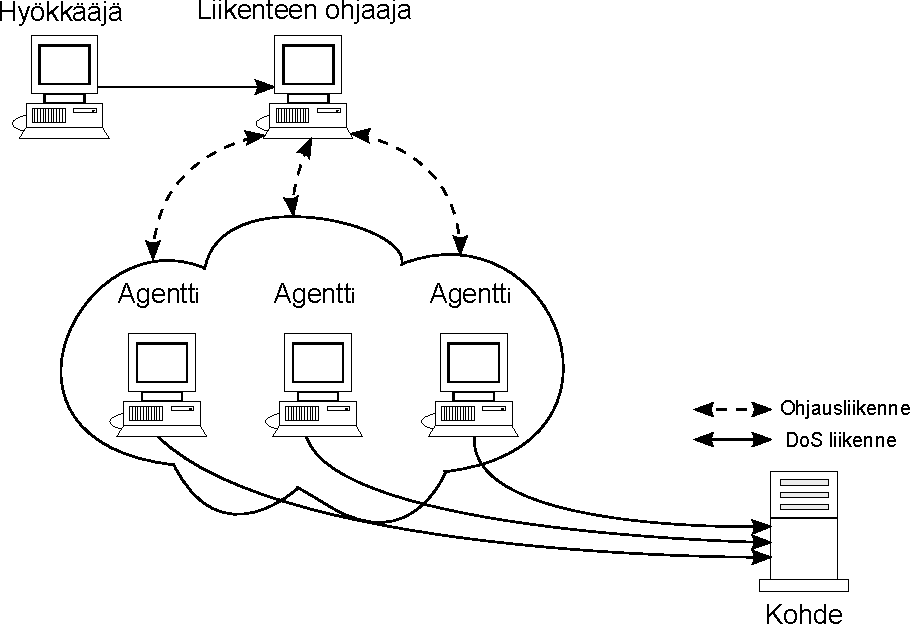
\includegraphics[width=12cm]{pics/perinteinen_ddos.pdf}
\caption{Perinteinen DDoS-verkosto}
\label{ddos1}
\end{figure}

Nykyisin enää harva DDoS-hyökkäyksessä käytetty verkko käyttää kuvan
\ref{ddos1} hierarkiaa sen heikon ohjattavuuden takia. Tämän tilalle
on tullut epäsuoraan käskyttämiseen perustuvat verkot, jotka käyttävät
viestien välittämiseen IRC-verkkoja (kuva \ref{ddos2}). IRC on
reaaliaikaiseen viestittämiseen tarkoitettu palvelu, jonka kautta
ihmiset pystyvät reaaliajassa kirjoittamaan ja lukemaan
viestejä. IRC-verkot koostuvat käyttäjistä ja IRC-kanavista, joille
käyttäjät voivat halutessana liittyä. Epäsuoran käskyttämisen
periaatteella toimivat verkot hyödyntävät näitä samoja
ominaisuuksia. Jokainen kone liittyy IRC-kanavalle, joka on yleensä
salasanalla suojattu. Kanavan kautta hyökkääjä voi antaa käskyjä
koneille. Tällä tavalla saadaan monia etuja verrattaessa suoraan
käskyttämiseen.  Ensinnäkin liikennettä ei pystytä enää tunnistamaan
poikkeavaksi, koska se on tavanomaista IRC-liikennettä. Toisekseen
käytettyä kanavaa voidaan vaihtaa lennosta, jolloin yhden kanavan
sulkeminen ei pysäytä verkon toimintaa. Näiden syiden takia
DDoS-hyökkäysten pysäyttäminen ennen niiden käynnistymistä on erittäin
vaikeaa \cite{DDOS}.

\begin{figure}[t]
\centering
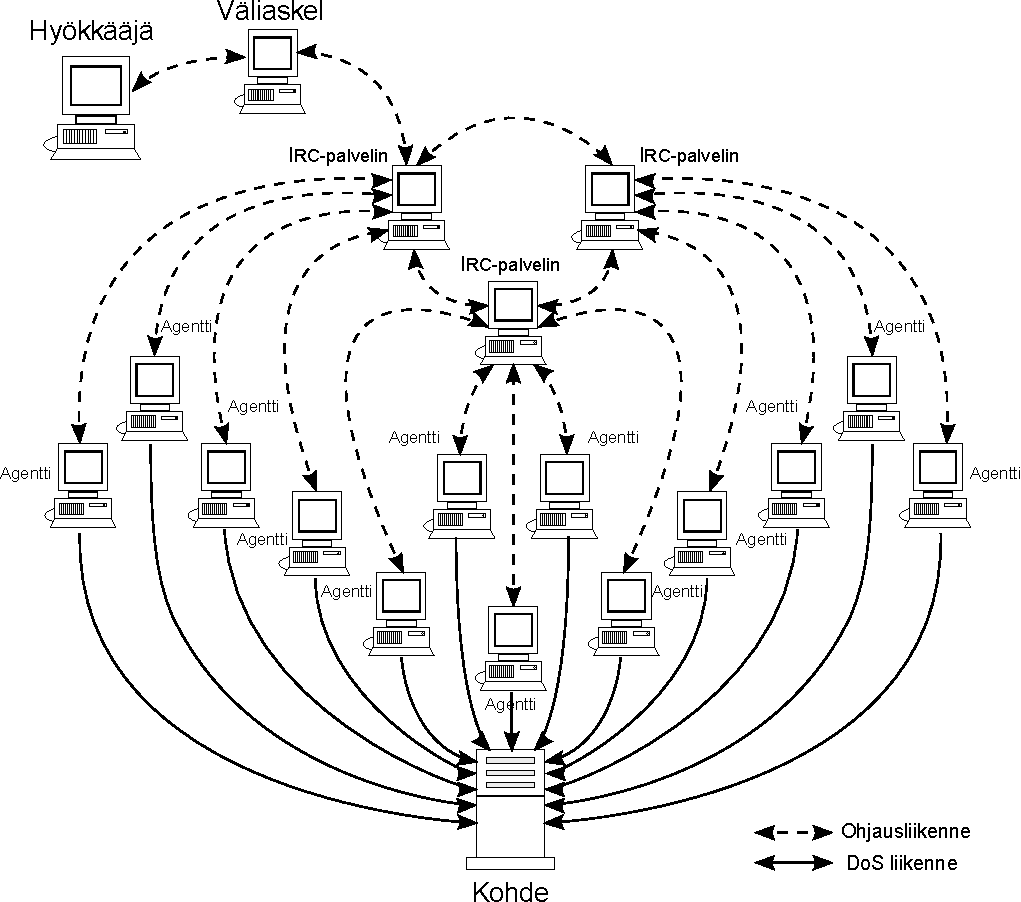
\includegraphics[width=12cm]{pics/ddos_uusi.pdf}
\caption{Nykyisin käytetty DDoS-verkosto}
\label{ddos2}
\end{figure}

% FIXME: Mitä hittoa seuraava kappale tarkoittaa?

Kuten yllä on jo tullut esille, on hajautetulta palvelunestohyökkäykseltä
suojautuminen vaikea tehtävä riippumatta siitä, onko verkko itse kohde vai
käytetäänkö sitä vain hyökkäysten koordinointiin. Valmista ja yksityiskohtaista
ratkaisua ei ole tarjolla, mutta seuraamalla joitakin yleisiä strategioita,
voidaan vahinkoja rajoittaa. Nämä strategiat ovat suojautuminen, tunnistaminen
ja reagoiminen, ja ne noudattavat vahinkoketjun yleistä elinkaarta \cite{DDOS}.

% FIXME: Pitäisikö tämä muutenkin siirtää jonnekin muualle, ei liity
% DDOSiin vaan tietoturvastrategioihin yleensä.

Ensinnäkin on tärkeää, että verkon ylläpitäjä tietää tarkoin kuinka verkko
toimii ja hyödynnetään verkon toimintaa analysoivia työkaluja. Näiden avulla
verkon heikot kohdat pystytään tunnistamaan ja vahvistamaan. Käytössä tulee
olla myös jonkinlainen suojausjärjestelmä, joka kirjaa ylös riittävän pitkältä
ajalta ylös verkkoon tulevan ja lähtevän liikenteen, sillä aina hajautettu
palvelunestohyökkäys ei kaada koko verkkoa. Tällöin on tärkeää, että tapahtunut
pystytään tarkasti analysoimaan ja löydetyt heikkoudet paikattua parhaalla
mahdollisella tavalla \cite{DDOS}.

Kun hyökkäys on meneillään, tulee käytetty hyökkäystapa tunnistaa mahdollisimman
nopeasti. Useimmat hyökkäykset noudattavat tiettyä kaavaa, ja näiden
tunnistamiseen on olemassa useita valmiita työkaluja. Tämä on tärkeää, koska
tunnistamisen jälkeen voidaan rajata, mistä hyökkäys on peräisin ja tehdä
tarvittavat toimenpiteet hyökkäyksen torjumiseksi. Useimmissa tapauksissa
tämä tarkoittaa yhteistyötä palveluntarjoajan ja viranomaisten kanssa.
Viranomaisten mukaan tuominen on muutenkin tärkeää, koska vain tätä kautta
voidaan käytettyä hyökkäysverkostoa lähteä tunnistamaan ja toivottavasti myös
hajottamaan \cite{DDOS}.

Jotta nopea reagoiminen olisi mahdollista, tulee organisaatiolla olla
toimintasuunnitelma hyökkäyksen varalta. Ensimmäinen vaihtoehto lienee aina
haitallisen liikenteen estäminen, mutta tätä varten tulee olla tehtynä tarkat
prosessit kuinka toimitaan hyökkäyksen alettua. Tärkeää on sopia mitä
dokumentoidaan ja kuinka asioista raportoidaan oikeille tahoille. Hyökkäyksen
jälkeinen analyysi on myös riippuvainen sovituista käytännöistä. Tämä analyysi
on erittäin tärkeää, sillä vain sitä kautta toimintasuunnitelmia voidaan
kehittää oikeaan suuntaan \cite{DDOS}.


\section{Remote-to-Local}

Remote-to-Local (lyh. \textit{R2L}) on hyökkäystyyppi, jossa hyökkääjä pyrkii
saamaan koneelle laajemmat oikeudet, kuin hänellä muuten
olisi. Tämä tapahtuu useimmiten käyttäen hyväksi järjestelmässä olevia
heikkouksia, joiden avulla hyökkääjä pääsee verkon yli murtautumaan
koneelle \cite{IDS}. Pahimmassa tapauksessa hyökkääjä saa hankittua koneelle
pääkäyttäjän oikeudet, jolloin koneen ja verkon resurssit ovat täysin
hyökkääjän käytettävissä.

Onnistuneet R2L-hyökkäykset ovat verkon ylläpitäjien kannalta pahimpia
mahdollisia, sillä niiden mahdollistamat tuhot ja aiheuttamat kustannukset ovat
huomattavasti suurempia verrattuna muihin hyökkäystyyppeihin \cite{IDSb}. Onnistunut R2L-hyökkäys saattaa
myös muut lähiverkon koneet vaaraan, sillä usein hyökkääjä pyrkii asentamaan
koneisiin ohjelmistoja, joiden avulla hyökkääjä pystyy ottamaan koneen haltuun
käyttäjän huomaamatta. Tällä tavoin osa aikaisemmin mainituista
zombverkostoista saa alkunsa.

Käytetyimmät Web-palvelinohjelmistot, Apache ja IIS, vastaavat noin 85~\%
kaikista käytetyistä palvelinsovelluksista. Näiden kahden lisäksi
BIND-\-ohjelmistoa käytetään valtaosassa nimipalvelimista. Ohjelmistojen yleisyydestä
johtuen yli puolet R2L-hyökkäyksen mahdollistavista heikkouksista onkin
löydetty näille alustoille \cite{IDS}. Useat haavoittuvaisuudet johtuvat
ohjelmointivirheistä, joiden johdosta hyökkääjä pystyy aiheuttamaan
sovellukseen muistin ylivuodon (engl. \textit{Buffer Overflow}). Tämä usein kaataa
sovelluksen tai saattaa sen sellaiseen tilaan, jossa hyökkääjä pystyy ajamaan
omia komentoja koneella. Kattava listaus löydetyistä haavoittuvuuksista ja näiden
korjauksista löytyy osoitteesta \url{www.cve.mitre.org/cve} \cite{CVE}.

Tunnetuilta R2L-hyökkäyksiltä suojautuminen on hyvin yksinkertaista, sillä
nykyinen trendi on, että haavoittuvuuden löytänyt taho ilmoittaa siitä
yleensä ensin
sovelluksen kehittäjille ennen julkista ilmoitusta. Siksi korjaus
haavoittuvuuteen on usein olemassa ennen kuin sitä on mahdollista hyödyntää \cite{IDSb}.
Vastuu jääkin verkon ylläpitäjälle, että käytetyt sovellukset ja 
suojausjärjestelmät pidetään ajan tasalla, sillä suurin osa onnistuneista hyökkäyksistä 
johtuu siitä, että tunnettuja tietoturva-aukkoja ei ole korjattu.

\section{User-to-Root}

User-to-Root (lyh. \textit{U2R}) hyökkäyksessä murtautuja pyrkii hankkimaan
koneelle pääkäyttäjän oikeudet. Tämä tapahtuu käyttäen järjestelmässä
olevia haavoittuvaisuuksia, joita ei ole paikattu. Useimmiten
hyökkäykset pohjautuvat koodausvirheisiin, jotka mahdollistavat
ylivuodon aiheuttamisen sekä odottamattomien syötteiden antamisen
\cite{IDS}. Käyttäjästä pääkäyttäjäksi hyökkäys eroaa R2L hyökkäyksestä
siten, että hyökkääjällä on jo valmiiksi pääsy koneelle tavallisen
käyttäjän oikeuksilla.

U2R-hyökkäykset ovat L2R-hyökkäysten ohella vaikeimpia torjua, jos kohteena
oleva järjestelmä on altis U2R-hyökkäyksille. Vaikea torjuttavuus johtuu siitä, että
usein hyökkäyksestä aiheutuva liikenne muistuttaa hyvin paljon normaalia
liikennettä, jonka vuoksi itsestään oppivat puolustusjärjestelmät eivät pysty
riittävän tarkasti erottamaan haitallista liikennettä normaalista \cite{U2R}.
Kehittyneimmilläkin järjestelmillä näiden hyökkäysten tunnistaminen on todella
heikkoa. Tämän on osoittanut useat eri tutkimushankkeet, jotka ovat käyttäneet
järjestelmiensä testaamiseen DARPAn simuloimaa verkkoliikennettä,
jossa olevat tietomurrot ja muu poikkeava toiminta on merkitty.
Parhaimmillaankin tunnistaminen on jäänyt 20 prosentin
paikkeille.

% -*- mode: LaTeX; coding: utf-8; -*-

\chapter{Web-palveluiden haasteet}

Toimivan ja ennen kaikkea turvallisen web-pohjaisen palvelun tarjoaminen vaatii
nykyisin todella paljon aikaa ja huolellisuutta niin palvelun kehittäjältä kuin myös
palvelun tarjoajalta ja ylläpitäjältä. Ajat ovat muuttuneet huomattavasti siitä,
jolloin käyttäjät selailivat pääasiassa vain staattisia web-sivuja, ja käyttivät tarjotuista
palveluista korkeintaan sähköpostia. Kehitys kulkee kovaa vauhtia eteenpäin, ja
tämän päivän suurimpia trendejä ovat ominaisuudet kuten interaktiivisuus,
sosiaalisuus ja yksilöllisyys, joiden avustuksella verkon käytöstä pyritään tekemään
käyttäjille entistä henkilökohtaisempi kokemus. Palvelut kuten MySpace,
Facebook ja YouTube ovat edelleen vahvistaneet näitä käyttäjätottumuksia, ja
markkinoille onkin syntynyt kova kilpailu siitä, kuka kehittää seuraavan
hittipalvelun. Nykyisin puhutaankin internetin seuraavasta evoluutiosta Web 2.0:
n muodossa, joita myös edellä mainitut palvelut edustavat. Uudet teknologiat ja
kiire tuovat kuitenkin aina mukanaan joukon uusia heikkouksia, joita hyökkääjät
pyrkivät hyödyntämään. Suunnittelijan ja ylläpitäjien kannalta onkin tärkeää, että 
kehityksen tuomiin haasteisiin pyritään vastaamaan mahdollisimman nopeasti ja tehokkaasti.

\section{Mitä tarkoittaa Web 2.0?}

Web 2.0 on termi, jota käytetään hyvin monessa eri tarkoituksessa ja
asiayhteydessä. Se yhdistetään esimerkiksi uusiin web-teknologioihin ja internet-
aikakauden tuotteiden/palveluiden kehityskaarien kuvaamiseen \cite{WEB2}. Yhteistä näille
on se, että ne pyrkivät esittämään sitä muutosta, jota internet pitää tällä
hetkellä sisällään. Tämä muutos on lähtöisin siitä, että kuluttajatottumukset
ovat kehittyneet kohti interaktiivisia palvelumalleja, joissa käyttäjillä on
entistä suurempi mahdollisuus vaikuttaa siihen, mitä informaatiota esitetään ja kuinka se esitetään.
Sosiaalisuus ja sen luoma yhteisöllisyys ovat luoneet tarpeen palveluille,
joissa käyttäjät pystyvät tekemään useita asioita saman aikaisesti saumattomasti
yhdestä paikasta käsin. Toinen kantava voima  muutokselle on ollut markkinoiden
tuoma paine, johon yritykset ovat pyrkineet mukautumaan niin kuluttajapuolella kuin myös
yrityspuolella. Tätä varten yritykset ovat kehittäneeet entistä suurempia ja 
monimutkaisempia kokonaisuuksia uusilla teknologioilla, joiden käyttöä ei aina hallita
riittävästi. Tähän kun lisätään kiire päästä markkinoilla ensimmäisten
joukossa, niin tietoturva jää usein taka-alalle \cite{WEB2b}.

Tietoturvan kannalta teknologiat, jotka luetaan kuuluvan osaksi Web 2.0
teknologiaperhettä, ovat jatkuvan huomion kohteena. Nämä teknologiat
muodostavat sen voiman, joka mahdollistaa siirtymisen interaktiivisiin
sovelluksiin kuten Google Maps, ja yritysten toiminnan siirtymisen verkkoon.
Teknologiat kuten Asynchronous JavaScript (AJAX), Cascading Style Sheet (CSS),
Flash, ActiveX ja XML voidaan kaikki laskea kuuluvan osaksi Web 2.0-perhettä.
Osa näistä teknologioista on ollut jo pidemmän aikaa käytössä, kun taas osaa on
vasta nyt alettu hyödyntämään siihen, mihin ne alun perin oli suunniteltu \cite{WEB2}.
Kuvassa \ref{web} on nähtävillä näiden yleisimpien teknologioiden ja protokollien
väliset suhteet.

\begin{figure}[htp]
\centering
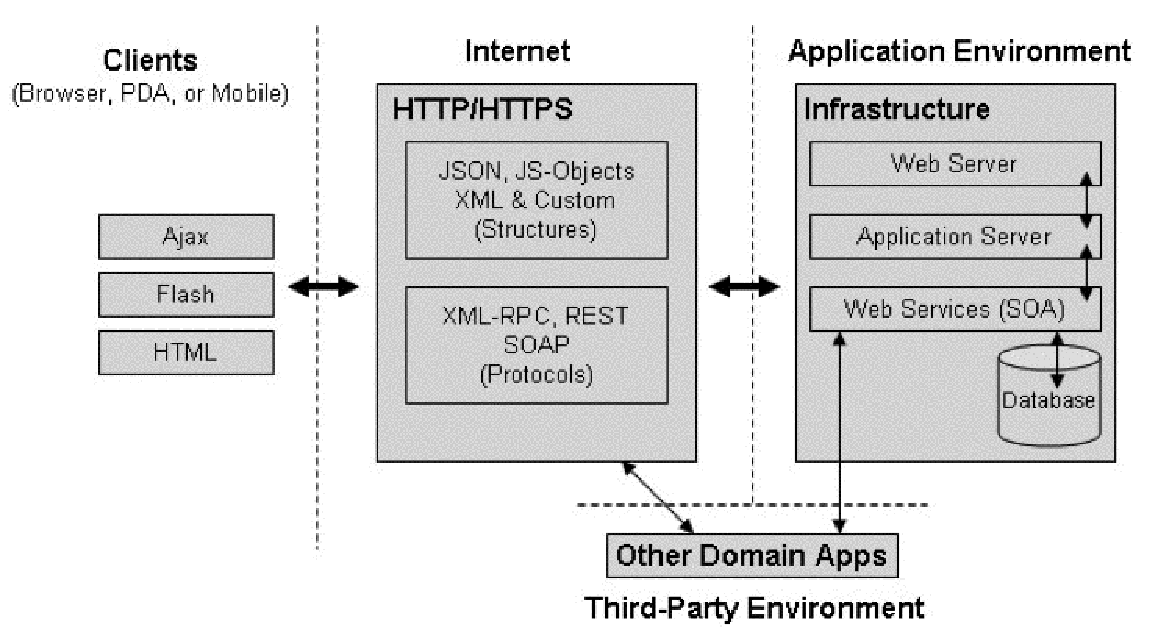
\includegraphics[width=12cm]{pics/web.pdf}
\caption{Web 2.0}
\label{web}
\end{figure}

Mitä Web 2.0 sitten tarkoittaa tietoturvan kannalta? Ensinnäkin se tuo mukanaan
samat vanhat haavoittuvuudet kuin mitä Web 1.0 sisälsi. Näiden lisäksi
hyökkäykset kuten Cross-site Scripting (XSS) ja Cross-site Request Forgery (
CSRF) ovat aikaisempaa vaarallisempia, koska käytetyt teknologiat tarjoavat
rikkaamman ympäristön, jonka kautta murtautua järjestelmiin \cite{WEB2}. Web 2.0
sovellukset antavat myös loppukäyttäjälle ja takana oleville ohjelmille enemmän
valtaa, jonka johdosta loppukäyttäjä ei välttämättä edes huomaa joutuessaan
tietomurron kohteeksi. Otetaan esimerkiksi Ajax-teknologia, joka mahdollistaa
sivujen tietojen päivittämisen käyttäen asynkronisia kutsuja. Näiden ansiosta
käyttäjä pystyy tekemään kutsuja palvelimille ja päivittämään osan sivun
tiedoista niin, ettei koko sivua tarvitse päivittää. Tästä suurin osa tapahtuu
käyttäjältä piilossa, joten hän ei todennäköisesti huomaa, jos selain lataa
haitallisia ohjelmia koneelle käyttäen jotain tunnettua haavoittuvuutta. Joidenkin
arvidoiden mukaan jopa 70 prosenttia kaikista haitallisista koodeista ladataankin käyttäen
Ajaxia \cite{WEB2c}.

Palvelinpuolella muutokset eivät rajoitu vain Web 2.0 tuomiin
tietoturvariskeihin, sillä uudenlainen ajattelu vaatii myös uudenlaisen
palveluarkkitehtuurin. Uusi arkkitehtuuriratkaisu tuo aina mukanaan suuren
joukon muutoksia, jotka tulee ottaa huomioon tietoturvaa suunniteltaessa.
Palvelukeskeinen arkkitehtuuri (engl. Service Oriented Architecture, SOA) on
yksi näistä kehysmalleista, joka on kasvattanut suosiotaan Web 2.0:n
vanavedessä. SOA-arkkitehtuurilla onkin nykyisin tärkeä rooli palvelujen
välisen kommunikoinnin kehittämisessä. Siksi onkin tärkeää ymmärtää mistä
palasista SOA-arkkitehtuuriin perustuvat palvelut koostuvat, ja mitä tämä
tarkoittaa turvallisuuden kannalta.

\section{Palvelukeskeinen arkkitehtuuri}

Web-pohjaiset teknologiat ovat saamassa yhä suurempaa huomiota yrityspuolen
sovelluskehityksessä. Tätä muutosta on ollut ohjaamassa teknologioiden
kehittyminen siihen pisteeseen, jossa yritykset pystyvät tarjoamaan aikaisemmin
asiakas-serveri sovelluksia verkon välityksellä luotettavasti ja nopeasti. Tämä
ratkaisu on tuonut mukanaan rahallisia säästöjä yrityksille, jotka ovat ennen
joutuneet itse huolehtimaan mm. sovellusten ajan tasalla pitämisestä ja
palvelimien ylläpitämisestä \cite{WEB2}. Muutos on luonut myös tarpeen löytää yhä
tehokkaampia kehitysmalleja ja tapoja toteuttaa entistä monimutkaisempia ja
vaativimpia sovelluksia suuryritysten tarpeisiin. Yksi tapa hallita tätä
muutosta on perustaa tehdyt ohjelmistosuunnitelman ratkaisut palvelukeskeisen
arkkitehtuurin malliin.

Puhuttaessa web-palveluista palvelukeskeinen arkkitehtuuri lähtee siitä
ajatuksesta, että palveluiden toiminnot ja prosessit pyritään suunnittelemaan
toimimaan mahdollisimman itsenäisesti ja avoimesti siten, että niitä pystytään
kutsumaan joustavasti eri sovellusten välillä käyttäen standardoitua rajapintaa.
Tähän ratkaisuun on ajanut pyrkimys laskea IT-kustannuksia ja maksimoida jo
käytössä olevien ratkaisujen uudelleenkäyttöä. Aikaisemmin tämän toteuttaminen
on ollut vaikeaa sovellusten heterogeenisyyden takia, jonka johdosta eri
alustojen ja toimittajien väliset yhteistoiminnot ovat olleet usein mahdottomia
toteuttaa. Yhä useamman sovelluksen ja palvelun siirtyessä verkkoon tästä
halutaan nyt päästä eroon, ja tähän ongelmaan palvelukeskeinen arkkitehtuuri
pyrkii tuomaan ratkaisun. Käytännössä tämä tarkoittaa sitä, että arkkitehtuurin
tulee tarjota sovelluksille mahdollisimman joustavan sekä sijainnista ja
protokollasta riippumattoman alusta \cite{SOA}. Tämän avulla loppukäyttäjälle
voidaan tarjota palveluita monesta eri paikasta yhtä aikaa siten, ettei hän ole
edes tietoinen tästä. Kyseessä on sama ajattelumalli johon Web 2.0 sovellukset
pohjautuvat, ja siksi palvelukeskeinen arkkitehtuuri onkin saanut paljon
nostetta Web 2.0:n myötä.

Palvelukeskeisen arkkitehtuurin tuomat edut eivät rajoitu pelkästään
kustannussäästöihin. Sen tuomiin etuihin kuuluvat myös mm. uusien toimintojen
helpompi integrointi jo käytössä oleviin järjestelmiin sekä monimutkaisten
kokonaisuuksien sujuvampi hallinta. Organisaatioille on myös tärkeää, että tällä
tavalla suunniteltuihin palvelumalleihin on nopeampi tehdä haluttuja muutoksia, jolloin 
reagointi markkinamuutoksiin voidaan toteuttaa nopeassa aikataulussa \cite{WEB2c}. Tämä on
erityisen tärkeää, koska markkinoille on ilmestynyt monia uusia tekniikoita,
jotka mahdollistavat web-palveluiden integroinnin jo käytössä oleviin
palveluihin. Onkin arvioitu, että vuonna 2008 web-pohjaisiin palveluihin
käytettiin jo yli 11 miljardia dollaria, ja osa fokuksesta on jo siirtynyt
kohti keskikokoisia ja pieniä yrityksiä. Web-pohjaisten palveluiden merkityksen
uskotaankin entisestään kasvavan ja yritykset, jotka reagoivat hitaasti tähän
muutokseen, huomaavat tulevaisuudessa olevansa epäsuotuisassa asemassa \cite{WEB2b}.

Palvelinpuolelle tapahtuva muutos tarkoittaa sopeutumista uudenlaiseen
ajattelumalliin, jossa palvelut on hajautettu ympäri verkkoa, ja joista osa ei
välttämättä ole saman ylläpitäjän hallinnassa. Kuvan \ref{soa} mukainen ratkaisu
tulee olemaan tulevaisuudessa arkipäivää, ja se tuo mukanaan uusia rajapintoja,
joiden kautta hyökkääjä voi pyrkiä murtautumaan järjestelmään tai jopa
yrityksen sisäiseen verkkoon. Koska palveluiden välinen kommunikointi perustuu
tässä mallissa luottamussuhteen luomiseen, tulee erityistä kiinnittää huomiota
siihen kuinka salaukset ja tunnistautuminen hoidetaan web-palveluita tarjoavien
osapuolien sekä käyttäjien kesken \cite{WEB2b}.

\begin{figure}[htp]
\centering
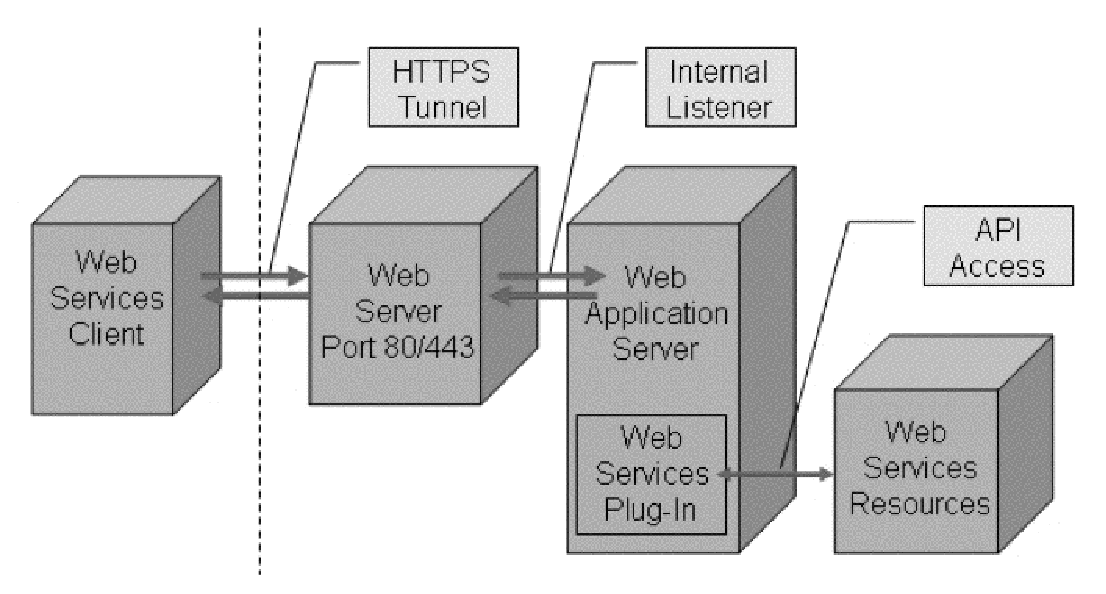
\includegraphics[width=12cm]{pics/soa.pdf}
\caption{SoA-arkkitehtuuri}
\label{soa}
\end{figure}

\section{Web-palveluiden tietoturva}

Internetin kehittyessä myös web-palveluihin kohdistuvat hyökkäykset ovat saaneet
uusia ilmenemismuotoja. Aikaisemmin ``web hakkerointia'' käytettiin kuvaamaan
hyökkäyksiä, jotka kohdistuivat palveluita tarjoaviin alustoihin kuten Apache, 
Microsoft IIS ja LAMP. Nämä hyökkäykset perustuivat tunnettujen haavoittuvaisuuksien
hyödyntämiseen, ja oikeille työkaluilla varustautunut hyökkääjä pystyikin kaatamaan haavoittuvan
palvelun muutamassa minuutissa. Esimerkiksi tunnetuimpien internet-matojen Code Redin ja Nimdan toiminta
perustui Microsoft IIS:sä olevan haavoittuvuuden hyödyntämiseen \cite{Hacking}. 

Tämänlaiset hyökkäykset ovat kuitenkin
menettäneet suurimman tehonsa, koska tehdyistä virheistä on opittu. Löydettyihin haavoittuvaisuuksiin
reagoidaan entistä nopeammin, yhä useampi alusta on konfiguroitu oikein ja saatavilla on työkaluja, joiden
avulla pystytään nopeasti ja helposti havaitsemaan yleisimmät tietoturvariskit \cite{Hacking}. Näistä seikoista johtuen
hyökkääjät ovatkin kiinnittäneet entistä enemmän huomiota itse alustalla pyöritettäviin palveluihin pyrkien 
murtautumaan järjestelmiin näiden kautta. Web 2.0:n myötä tämän tyyppiset hyökkäykset ovat saaneet entistä
enemmän huomiota, sillä se on tarjonnut hakkereille entistä monipuolisemman hyökkäyspinnan. Tietoturvan 
kannalta onkin tärkeää, että kumpaankin hyökkäystapaan kiinnitetään huomiota.

\subsection{Web-palvelimien turvaaminen}

Yllä mainitut seikat eivät tarkoita sitä, että web-palveluita pyörittävät alustat olisivat
turvassa hyökkäyksiltä. Onnistuneet hyökkäykset ovat edelleen yhtä tuhoisa, jos niihin ei varauduta ennalta.
Nämä erilaiset hyökkäykset pyrkivät yleensä hyödyntämään seuraavissa kategorioissa olevia heikkouksia

\begin{itemize}
\item Valmiit esimerkkitiedostot
\item Lähdekoodin paljastuminen
\item Kanonisointi
\item Palvelmiin asennetut lisäosat
\item Syötteen tarkistaminen \cite{Hacking}.
\end{itemize}

Näiltä suojautuminen on melko yksinkertaista, kunhan muistaa noudattaa muutamaa pääperiaatetta. Ensinnäkin tuotannossa 
olevilla palvelimilla ei tulisi koskaan olla asennettuna tai käytettynä tiedostoja, joiden turvallisuudesta ei ole
takeita. Näihin tiedostoihin kuuluvat mm. paketeissa mukana tulevat esimerkkitiedostot ja palvelimelle asennettavat 
lisäosat, joiden alkuperästä ei ole varmuutta. Toisekseen on tärkeä varmistaa, että käytettyihin sovelluksiin
on asennettu viimeisimmät päivitykset, sillä ne yleensä korjaavat tunnetut heikkoudet \cite{Hacking}. Jo pelkästään näillä 
toimilla pystytään suurimmaksi osaksi estämään palvelmiin kohdistuvat hyökkäykset. 

\subsection{SQL injektio}

Virheelliseen syöttötietoon perustuvat hyökkäykset ovat jo pidemmän aikaa vaivanneet web-pohjaisia sovelluksia.
Web 2.0:n myötä hyökkäykset ovat entisestään yleistyneet, sillä monimutkaisten sovellusten takana käytetään entistä
enemmän erilaisia tietokantapohjaisia ratkaisuja kuten MySQL. Nämä hyökkäykset hyödyntävät sitä seikkaa, että suurin osa
sovelluksista ei tee selkeää eroa käyttäjän antaman syötteen ja ohjelmalle annettavien ohjeiden välillä. Tämä mahdollistaa
sen, että hyökkääjä pystyy piilottamaan annettuun hakuun ohjelmatason käskyjä, jotka muokkaavat sovelluksen toimintaa
hyökkääjän haluamaan suuntaan \cite{WEB2}. Normaaleilla toimenpiteillä tällaisen hyökkäysten tunnistaminen on hankalaa, sillä
yritysten tietoturvasta vastaavat palomuurit toimivat OSI-mallin kolmannella, neljännellä ja viidennellä kerroksella, eivätkä
näin ollen tunnista ylimmän tason eli ohjelmistotason kautta tulevia hyökkäyksiä. Tämän lisäksi useimmat palomuurit eivät ymmärrä protokollien
kuten HTTP:n tarkkaa sisältöä \cite{SQLSS}.

Onnistunut injektiohyökkäys koostuu kolmesta erillisestä vaiheesta. Ensimmäisessaä vaiheessa hyökkääjän tulee tunnistaa 
web-sovelluksessa käytetyt teknologiat. Tämä onnistuu mm. tulkitsemalla sivujen antamia virheilmoituksia, tutkimalla 
sivun lähdekoodia ja käyttäen tätä varten tehtyjä työkaluja kuten Nessus ja Nmap. Tämä vaihe on hyökkääjälle melko triviaali
tehtävä, mutta hyökkäyksen kannalta tiedot ovat elintärkeitä, sillä injektiohyökkäyksen onnistuminen on täysin riippuvainen 
käytetystä ohjelmointikielestä. Kun tarvittavat tiedot on saatu kerättyä, voidaan varsinaista hyökkäystä alkaa suunnittelemaan.
Tämä tapahtuu tunnistamalla ne syötteet, jotka käyttäjä pystyy sovellukselle antamaan. Tämä käsittää käytännössä kaiken sen 
datan, joka kulkee HTTP GET ja HTTP POST pyynnöissä. Viimeisessä vaiheessa hyökkääjän tehtäväksi sitten jää niiden syötteiden 
tunnistaminen, joita käyttämällä sovelluksen toimintaa saadaaan muokattua. Tähänkin tehtävään löytyy useita valmiita työkaluja, ja
monessa tapauksessa samat toimintaperiaatteet toimivat eri sovellusten välillä \cite{WEB2}.

Structured Query Language (lyh. SQL), joka on alan de facto standardi tietokantojen käsittelyyn, on käytössä lähes jokaisessa
web-sovelluksessa, joka käyttää jonkinlaista tietokantaratkaisua. Sen syntaksi on sekoitus ohjelmakäskyjä ja käyttäjän antamia
syötteitä, ja huonosti määritettynä käyttäjän antama syöte voidaan tulkita virheellisesti ohjelmatason käskyksi. Tämän syötteen
hyökkääjä joutuu usein etsimään sokeasti, mutta syötteet kuten

\begin{itemize}
\item ' OR 1=1 "{-}{-}
\item ') OR 1=1 "{-}{-}
\end {itemize}
toimivat hyvin usein \cite{WEB2}. Virheellisestä hausta aiheutuvat virheilmoitukset antavat myös erittäin paljon
hyödyllistä tietoa hyökkääjälle \cite{SQLSS}. Koska suurin osa SQL-tietokannoista mahdollistaa useamman perättäisen syötteen 
antamisen, kunhan syntaksi pysyy oikeana, voidaan näiden avulla katkaista ohjelman normaali toiminta. Otetaan esimerkiksi SQL-haku
\begin{tt}
\begin{center}
String query= ``SELECT id FROM user\_table WHERE `` + \\
``username = ' `` + username + ``' AND `` + \\
``password = PASSWORD(' `` + password + ``')''; \\
\end{center}
\end{tt}
Antamalla käyttäjänimeksi arvon

\begin{tt}
\begin{center}
' OR 1=1; DROP TABLE user\_table;"{-}{-}
\end{center}
\end{tt}
muuttuu tietokannalle ohjautuva kysely muotoon

\begin{tt}
\begin{center}
String query= ``SELECT id FROM user\_table WHERE username=' ' OR 1=1; DROP TABLE
user\_table; "{-}{-} ' AND password = PASSWORD ('x');
\end{center}
\end{tt}
SQL-kielessä kaksi perättäistä viivaa tarkoittaa, että kaikki siitä oikealla puolella oleva on kommenttia. 
Näin ollen lopullinen SQL-haku on 

\begin{tt}
\begin{center}
String query= ``SELECT id FROM user\_table WHERE \\username=' ' OR 1=1; DROP TABLE
user\_table;
\end{center}
\end{tt}
Näin muodostettu haku on syntaktisesti täysin oikea, ja se tyhjentää tietokannassa olevan user\_table tiedoston, joka pitää
sisällään järjestelmään tallennetut käyttäjät \cite{WEB2}. 

Vastaavanlaisia tekniikoita käyttäen hyökkääjä pystyy tekemään kaiken sen, joka pystytään esittämään SQL-kyselynä, ja johon ajettavalla
sovelluksella on riittävät oikeudet. Mielivaltaisten käskyjen antaminen, DLL tiedostojen luominen ja ajaminen ja tietokannan
sisällön lähettäminen jollekin toiselle internetissä olevalle palvelimelle ovat vain muutamia esimerkkejä toiminnoista, joita
onnistunut hyökkäys voi aiheuttaa \cite{SQLSS}.

Injektiohyökkäykset eivät rajoitu pelkästään SQL-kieleen, sillä useat eri tekniikat kuten XPath ja LDAP sisältävät vastaavanlaisia 
heikkouksia \cite{WEB2}. SQL-kieleen pohjautuvat hyökkäykset ovat kuitenkin kaikista yleisimpiä johtuen sen levinneisyydestä. SQL-kieleen
pohjautuvat ratkaisut sisältävät usein myös osan seuraavista ominaisuuksista, jotka mahdollistavat hyökkäysten tekemisen:

\begin{itemize}
\item Kommentoinnin mahdollistavat merkki: "{-}{-}.
\item Mahdollisuus suorittaa useita hakuja yhdellä kertaa käyttäen puolipistettä.
\item SQL-palvelimen antamat tarkat virheilmoitukset
\item Syötteen tyypin ehdoton kääntäminen -- kokonaisluvut käännetään mahdollisuuksien mukaan merkkijonoksi, jolloin hyökkääjän
             on helpompi arvata oikea syöte \cite{SQLSS}.
\end{itemize}

Esille tulleiden asioiden valossa on selvää, että SQL-kieleen pohjautuvat haavoittuvaisuudet ovat todellinen uhka yritysten tietoturvalle.
Tästä johtuen on tärkeää, että sovellusten turvallisuus pyritään takaamaan kaikin mahdollisin tavoin. Täysin turvallisen sovelluksen 
suunnitteleminen on kuitenkin lähes mahdoton tehtävä, mutta noudattamalla muutamia perusperiaatteita voidaan riskiä vähentää huomattavasti.
Vastaavasti myös palvelinpuolella SQL-injektiohyökkäykset tulee ottaa huomioon suunniteltaessa verkon tietoturvaratkaisuja.

Koska injektiohyökkäykset pyrkivät hyödyntämään syötteiden virheellistä tulkintaa, voi hyväksyttävien syötteiden rajoittaminen tuntua
helpolta ratkaisulta ongelmaan. Osittain tämä ratkaiseekin asian, mutta ongelmaksi muodostuu se, kuinka valita mikä syöte on hyväksyttävä
ja mikä virheellinen. Tämän valitsemiseen on useita eri tapoja kuten esimerkiksi sallia ainoastaan syötteet, jotka tiedetään etukäteen hyväksi
ja huonon syötteen riisuminen tai pois tiputtaminen. Näistä tavoista ensimmäinen on kaikista rajoittavin, koska tällöin syötteen jokainen 
merkki tarkistetaan, ja jos se ei ole sallittujen merkkien joukossa niin koko haku hylätään. Huonojen syötteiden riisuminen on myös vaikea
toteuttaa, koska harvoin pystytään määrittelemään mikä haku on huono ja mikä hyvä. Yksi hyväksi todettu tapa onkin rajoittaa tiettyjen
merkkien käyttöä siten, että merkin ollessa haussa mukana tämä muutetaan toiseen muotoon. Tämäkään ratkaisu ei ole täysin ongelmaton, ja siksi
viisainta onkin vain hylätä koko syöte, jos se ei vastaa odotettua syötettä \cite{SQLSS}.

Palvelinpuolella tulee myös ottaa huomioon muutamia asioita, joita seuraamalla voidaan huomattavasti parantaa yrityksen tietoturvaa.
Palvelinpuolen ratkaisuilla voidaan myös pienentää huonosti suunnitellun sovelluksen riskiä joutua injektiohyökkäyksen kohteeksi. 
Seuraava lista ei ole millään tavalla täydellinen ratkaisu ongelmaan, mutta se antaa osviittaa siitä, millä tavoin riskiä voidaan vähentää:

\begin{itemize}
\item SQL-palvelimen ajaminen pienillä käyttöoikeuksilla.
\item Sallia tallennettujen proseduurien ajaminen ainoastaan järjestelmän ylläpitäjille
\item Linkitettyjen palvelimien yksinkertaisten tunnistusten poistaminen
\item Määrittää palomuuri siten, että ainoastaan luotetut käyttäjät saavat ottaa yhteyden SQL-palvelimeen. Usein ainoat, joiden yhteydet 
      tulee sallia, ovat ylläpitäjät ja web-palvelut, joita tietokanta palvelee \cite{SQLSS}.
\end{itemize}

\subsection{Cross-site Scripting}
Nykyisin yhä useampi yritys on tietoinen verkon tarjoamista mahdollisuuksista ja sen mukana tulevista vaaroista. Yritykset ovat tämän johdosta
alkaneet panostamaan entistä enemmän tietoturvaan, ja harva toimiikin enää ilman kunnollista suojausta. Palomuurit ja hyökkäysten tunnistamiseen
ja estämiseen erikoistuneet sovellukset ovat myös kehittyneet viime vuosina niin paljon, että enää harva perinteinen hyökkäys toimii ilman
suuria muutoksia sen toteutustapaan. Tästä johtuen hakkerit ovat alkaneet omaksumaan yhä salamyhkäisempiä hyökkäystapoja, jotka pyrkivät kokonaan
ohittamaan perinteiset palomuurit. Web-pohjaiset sovellukset tarjoavat tähän erinomaisen alustan, ja Web 2.0:n myötä mahdollisuudet vain kasvavat
entisestään.

Cross-site scripting eli XSS-hyökkäykset eivät ole millään tapaa uusi hyökkäystyyppi, ja joidenkin arvioiden mukaan kahdeksan kymmenestä sivustosta on 
sille jollakin asteella alttiina. XSS-hyökkäykset ovat kuitenkin viime vuosina keränneet suurempaa huomiota hakkereiden keskuudessa, sillä Web 2.0 sovellusten
myötä yhä useampi näistä käyttää erilaisia tiedonlähteitä sisällön keräämiseen. RSS-feedit, widgetit, moduulit ja erilaiset JavaScript-pohjaiset komponentit 
tarjoavat kaikki hyökkääjälle monta mahdollisuutta, johon iskeä. Tähän kun vielä lisätään se, että sovelluksista monet päivittävät tietoja käyttäjän tietämättä, 
niin tilanteesta muodostuu entistä vaarallisempi \cite{WEB2b}. Tästä johtuen XSS-hyökkäykset muodostavat nyt ja tulevaisuudessa erittäin suuren riskin
tietoturvalle.

Painotuksen siirtyminen web-pohjaisiin hyökkäyksiin on ollut selkeästi havaittavissa jo pidemmän aikaa. Vuonna 2007 johtava tietoturva-alan 
yritys Symantec julkisti raportin, jonka  mukaan vuoden 2007 viimeisen kuuden kuukauden aikana raportoiduista haavoittuvaisuuksista 11,253
oli sivustokohtaisia cross-site scripting tietoturva-aukkoja. Tätä lukua kun vertaa muihin löydettyihin riskeihin, joita oli 2,134, niin 
yli 80 prosenttia löydetyistä tietoturva-aukoista oli web-pohjaisia \cite{SYM}. Vuonna 2009 julkistetussa raportissa tilanne on edelleen sama, 
sillä 63 prosenttia haavoittuvaisuuksista kohdistui Web-sovelluksiin \cite{SYM2}.

Kuten aikaisemmin on jo tullut esille, niin injektiohyökkäykset eivät rajoitu pelkästään tietokantasovelluksiin. Myös XSS-hyökkäykset ovat eräänlaisia 
injektiohyökkäyksiä sillä erotuksella, että hyökkääjä ei suoraan toteuta injektiota vaan uhri tekee sen itse. Tähän hyökkääjällä on useita eri 
keinoja, ja harvoin käyttäjä edes huomaa joutuneensa hyökkäyksen kohteeksi. Hyökkäyksen onnistuessa web-sivujen käyttämä ``saman alkuperän'' periaate
voidaan kiertää, jolloin hyökkääjän on mahdollista ajaa kohteen selaimessa haluamaansa koodia ja skriptejä. Tämä ``saman alkuperän'' periaate on 
web-selainten yksi tärkeimmistä suojausmenetelmistä, ja se estää mm. skriptien lataamisen yhdestä lähteestä hakemalla tai asettamalla määrityksiä 
toisesta lähteestä \cite{WEB2}. Hyökkäys voidaan esimerkiksi toteuttaa siten, että haavoittuvalle web-sivustolle asennetaan vihamielinen skripti.
Tämä skripti on usein kirjoitettu JavaScriptillä, ja käyttäjän vieraillessa sivustolla se ajetaan käyttäjän web-selaimessa. Koska selain luottaa siihen, 
että sivuston sisältö on luotettavasta lähteestä, pystyy hyökkääjä lukemaan ja muokkaamaan arkaluontoista sisältöä. Evästeet, jotka ovat web-sovellusten 
toiminnan kannalta erittäin tärkeitä, ovat ensimmäisiä kohteita, joihin yritetään yleensä päästä käsiksi,  sillä ne pitävät yllä yhteyksien tiloja eri 
sivustoille ja oikean käyttäjän tunnistamiseen tarvittavia tietoja \cite{WEB2b}. Näitä kaappaamalla hyökkääjä pystyy esiintymään verkossa toisena käyttäjänä, 
ja väärinkäyttämään palveluita kuten verkkopankkia tai webmailia. Hyökkäys voidaan myös toteuttaa huijaamalla käyttäjä klikkaamaan vihamielistä linkkiä, 
joka aktivoi HTML-pohjaisen skriptin \cite{WEB2}.

Hyökkääjän mahdollisuudet eivät rajoitu pelkästään evästeiden varastamiseen. Onnistuneen XSS-hyökkäyksen jälkeen hakkeri voi esimerkiksi ohjata
käyttäjän osoitteeseen, joka jäljittelee haluttua sivustoa. Käyttäjän sitten yrittäessä kirjautua palveluun, saa hyökkääjä selville käyttäjän tunnuksen ja
salasanan. XSS-hyökkäykset tarjoavatkin erinomaisen mahdollisuuden toteuttaa phishing eli tiedon kalasteluhyökkäyksiä. XSS-madot ovat
myös viime aikoina yleistyneet, sillä yhä useampi palvelu on niille haavoittuvainen. Esimerkiksi webmail-sovelluksia varten kirjoitetut madot 
käyttävät hyödyksi sitä seikkaa, että hyökkääjä pääsee käsiksi uhrin kontaktilistaan. Tällainen mato pyrkii leviämään lähettämällä 
kontaktilistalla oleviin osoitteisiin sähköpostia, ja koska viesti tulee luotettavasta osoitteesta, ei käyttäjät osaa usein varoa viestissä
olevaa linkkiä. Hyökkääjä vielä usein muokkaa linkistä sen näköisen, että vastaanottaja ei osaa epäillä linkin aitoutta \cite{WEB2}. 
XSS-madot leviävätkin usein todella nopeasti, ja ne kuljettavat usein myös muita hyökkäyksiä mukanaan. Tästä hyvänä esimerkkinä
Sammy-madoksi nimetty XSS-hyökkäys, joka vuonna 2005 iski MySpace-sivustolle, joka on yksi tunnetuimmista sosiaaliseen verkoistutumiseen
erikoistuneista sivustoista. Käyttäen sivustossa olevaa heikkoutta hyväkseen mato saastutti käyttäjien sivuja, ja jonkun vieraillessa 
saastuneella sivulla, saastui myös hänen oma MySpace sivunsa. 24 tunnissa mato oli saastuttanut yli miljoona sivua, ja tilanteen korjaamiseksi
MySpace joutui sulkemaan sivustonsa. Hyökkäyksen vahingot eivät rajoittuneet tähän vaan seuraavina viikkoina useista tunnetuista sivustoista
kuten Google ja Yahoo löytyi vastaavanlaisia heikkouksia \cite{WEB2b}.

Tärkein asia XSS-hyökkäysten estämiseksi on olla hyvin tarkkana sen suhteen, kuinka käyttäjien tarjoama sisältö välitetään toisille käyttäjille.
Tärkeää on myös muokata käyttäjän antama syöte aina sellaiseen muotoon, että kun palvelin lähettää esimerkiksi virhesanomassa käyttäjän antaman syötteen
takaisin, niin ei tätä voida käyttää sellaisenaan hyökkäyksen toteuttamiseen. Tiettyjen merkkien poistamisella voitaisiin hyökkäyksi vähentää,
mutta usein merkkien kuten heittomerkin (') poistaminen ei tule kyseeseen. Suunnittelijoiden avuksi on myös olemassa suuri määrä sovelluksia, jotka
etsivät sivustoilla olevia heikkouksia \cite{WEB2}. Tämän suhteen tulee kuitenkin muistaa, että myös hakkereilla on käytettävissä samat sovellukset, joten 
löydetyt heikkoudet tulisi korjata mahdollisimman nopeasti. Symantecin raportin mukaan näin kuitenkin tapahtuu todella harvoin, sillä 6,961 
sivustosta vain 473 oli korjattu raportin kirjoittamisen aikana ja tähänkin oli mennyt keskimäärin 52 päivää \cite{SYM}. XSS-haavoittuvista sivuista
kirjaa pitävän sivuston mukaan tilanne ei ole nykyisin yhtään sen parempi, sillä suurin osa löydetyistä sivuista on edelleen korjaamatta \cite{XSS}.
Näyttääkin siltä, että yritykset ymmärtävät asian vakavuuden vasta sitten, kun sivusto on joutunut hyökkäyksen kohteeksi.

\subsection{Cross-site Request Forgery}

Web 2.0 sovellusten yksi keskeisimmistä asiakaspuolen ratkaisuista on Document Object Modeliksi (lyh. DOM) nimetty ohjelmointirajapinta, joka on vastuussa siitä, 
kuinka web-sivun sisältöä käsitellään ja kuinka eri objektit kommunikoivat keskenään. Rajapinta vastaa siitä, että ainoastaan saman domainin 
sisäinen kommunikointi ja sisällön muokkaaminen on sallittua. Tämä ratkaisu poistaa sen mahdollisuuden, että web-sivun DOM:ia voitaisiin muokata toisen
domainin kautta. Tämä vastaa ``saman alkuperän'' periaatetta, jolla pyritään estämään web-sivuihin ja käyttäjiin kohdistuvia vihamielisiä toimia.
Webin muuttuessa entistä interaktiivisemmaksi, ovat sivut kuitenkin alkaneet sallia yhä enemmän domainien välistä kommunikointia. Tällaisia 
toimia ovat esimerkiksi hyperlinkkien käyttäminen sisällön näyttämisessä, kuvien ja objektien lataaminen sekä toisessa domainissa olevien 
JavaScriptien ajaminen. Nämä ja monet muut toimet ovat mahdollistaneet entistä monipuolisempien web-palveluiden suunnittelun, mutta huonosti toteutettuna 
ne jättävät palvelut hyvin haavoittuviksi. Tämä johtuu siitä, että käyttäjän tarkoituksella tekemiä toimia ei pystytä erottamaan niistä toimista, jotka tehdään 
automaattisesti käyttäjän vieraillessa sivustolla \cite{WEB2}.

XSS-hyökkäysten tapaan myös Cross-site Request Forgery (lyh. CSRF) hyökkäykset ovat jo pidemmän aikaan olleet olemassa, mutta vasta Web 2.0:n myötä ne
ovat alkaneet yleistymään. Ero näiden kahden hyökkäyksen välillä on siinä, että missä XSS skripti suoritetaan käyttäjän selaimessa, niin CSRF hyökkäyksessä käytetyt
käskyt ja skriptit kohdistetaan luotettuihin web-palveluihin. CSRF toteutetaan siten, että hyökkääjä asettaa jollekin sivulle vihamielisiä tageja, joiden
avulla voidaan luoda mielivaltaisia HTTP pyyntöjä. Nämä pyynnöt sitten kohdistetaan johonkin toiseen domainiin, ja ne ajetaan käyttäjän vieraillessa kyseisellä 
sivulla. Jos käyttäjän selaimella on sitten esimerkiksi tähän domainiin liittyvä eväste voimassa, voidaan HTTP pyynnöillä pyytää mm.  salasanan vaihtoa 
tai sähköpostin lähettämistä käyttäjän nimissä \cite{WEB2b}. Hyökkääjä pystyy tällä tavoin myös ottamaan yhteyttä sellaisiin koneisiin ja palveluihin, joihin 
hänellä ei muuten olisi oikeuksia johtuen esimerkiksi palomuurista tai IP-osoitteiden suodatuksesta \cite{CSRF}.

CSRF hyökkäysten teho perustuu siihen, että monet sivustot ja palvelut käyttävät evästeitä melko huolimattomasti. Koska näiden avulla sivustot autentikoivat tulevat 
HTTP pyynnöt niin riittää, että hyökkääjä pääsee niihin käsiksi tavalla tai toisella. Useat sivustot myös sallivat käyttäjien pysyvän kirjautuneena sisällä
jopa useita viikkoja, jolloin sama eväste on pitkään käytössä. Monien sovellusten ja pyyntöjen rakenne on myös hyvin ennalta arvattavissa, jolloin hyökkääjän
on helpompi arvata käskyjen ja parametrien oikea muoto \cite{WEB2}.

CSRF hyökkäykset eivät rajoitu pelkästään perinteisiin web-tekniikoihin, sillä suurin osa Web 2.0:n mukana tuomista teknologioista on sille jollakin 
tavalla alttiina. Erityisesti AJAX ja JavaScript ovat tuoneet mukanaan suuren joukon uusia haasteita, jotka suunnittelijoiden tulee ottaa huomioon uusien
sovelluksien suunnittelussa. \cite{WEB2b}. Täydellinen suojautuminen CSRF hyökkäyksiltä vaatiikin sellaista syvällistä osaamista käytetyistä tekniikoista ja 
tietämystä eri komponenttien välisistä toimininnoista, jota harvalta löytyy. Siksi iso osa sivustoista ja palveluista onkin haavoittuvaisia eri asteisille
CSRF hyökkäyksille. Tästä hyvänä esimerkkinä tunnettu sähköpostisivusto Gmail, josta löytyi vuonna 2007 CSRF hyökkäyksen mahdollistava heikkous. Tämän avulla
hyökkääjän oli mahdollista luoda Gmailiin sellainen suodatus, joka ohjasi tulevat postit toiseen osoitteeseen \cite{CSRF}. 

CSRF hyökkäyksiltä suojautumiseen on käytössä kolme hyvin yleistä tekniikkaa. Näistä käytetyin on sisällyttää jokaiseen serveripuolen dataa muokkaavaan
GET/POST pyyntöön mukaan salattu tokeni, jonka avulla jokainen pyyntö voidaan yksilöidä ja tunnistaa kuuluvan oikeaan istuntoon. Tämä salattu tokeni tekee
käyttäjän syötteestä arvaamattoman muotoisen, jonka johdosta CSRF-hyökkäyksen toteuttaminen on hyvin vaikeaa \cite{WEB2}. Yksinkertaisin suojausmenetelmä on 
taas tunnistaa HTTP pyynnön Referer otsake, ja hyväksyä vain sellaiset pyynnöt, jotka tulevat luotettavista lähteistä. Kolmas menetelmä on tehdä kustomoituja
otsakkeita käyttäen XMLHttpRequestia, jonka käyttö on lisääntynyt AJAXin yleistyessä. Kustomoitujen otsakkeiden oikeellisuus sitten varmistetaan, ennen kuin
pyynnöt käsitellään palvelinpuolella \cite{CSRF}.

Nämä kolme esitettyä tapaa ovat yleisimmin käytössä, mutta nekin sisältävät joukon heikkouksia. Salatun tokenin ongelma on siinä, että kyseisestä tekniikasta ei 
ole olemassa yleisesti sovittua toteutustapaa. Tämä aiheuttaa sen, että useat ratkaisut ovat tavalla tai toisella puutteellisia. Referer otsakkeiden suodatuksen 
ongelma on siinä, kuinka käsitellä pyyntöjä, joista puuttuu Referer otsake. Otsakkeen piilottaminen ei ole vaikea tehtävä, joten palvelin saattaa joutua 
päättämään vajailla tiedoilla päästääkö pyyntö läpi vaiko suodattaa se pois. XMLHttpRequestin käyttöä taas rajoittaa sen tuomat lisävaatimukset toteutukselle,
joka rajoittaa tiettyjen palveluiden käyttöä \cite{CSRF}. 

Näiden ja monien muiden syiden takia tutkimustyö CSRF hyökkäysten parissa on kasvattanut suosiotaan. Esimerkiksi yhdessä tutkimuksessa ehdotettiin erillisen Origin
otsakkeen lisäämistä pyyntöön, joka korjaisi Referer kentän heikkoudet \cite{CSRF}. Toisessa tutkimuksessa taas pyrittiin kasvattamaan web-selaimen turvallisuutta
lisäämällä selaimeen mekanismi, joka pyrki arvioimaan vastasiko tehdyt pyynnöt käyttäjän toimia \cite{CSRFb}. Näistä kahdesta ratkaisusta on kuitenkin nähtävissä se,
että tutkimuskenttä CSRF hyökkäysten ympärillä on vielä hyvin alkuvaiheessa, ja vastuu riittävän suojauksen hoitamisesta jääkin vielä tällä hetkellä 
sovelluksen kehittäjälle ja ylläpitäjälle.

\section{Web-palveluiden turvaaminen}

Web-palveluiden tietoturvasta vastaaminen on tarkkuutta ja aikaa vaativaa työtä, joka edellyttää omien tietojen jatkuvaa päivittämistä sekä ja liikenteen ja palveluiden
seuraamista. Jo pelkästään yleisimpien tietoturvariskien tunnistaminen ja korjaaminen osoittautuu usein käsin tehtynä ylivoimaiseksi tehtäväksi palveluiden
muuttuessa entistä monimutkaisemmaksi. Onneksi työn helpottamiseksi on saatavilla useita erilaisia työkaluja, joiden avulla sekä kehittäjät että ylläpitäjät voivat
etsiä sovelluksista tunnetuimpia tietoturva-aukkoja. Osa näistä pohjautuu vapaaseen lähdekoodiin, mutta tarjolla on myös kaupallisia sovelluksia, jotka ainakin 
paperilla lupaavat parempia ominaisuuksia. Näiden lisäksi myös palvelinpuolella on tarjolla erilaisia lisäosia, jotka lisäävät web-palveluiden tietoturvaa. 
Mikään sovellus ei tietenkään voi löytää kaikkia mahdollisia heikkouksia, joten pelkästään näiden varaan ei sovelluksen turvallisuutta voi laittaa. Näiden avulla 
saadaan kuitenkin hyvä yleiskuva siitä, minkälaisille heikkouksille sovellus on mahdollisesti alttiina ja kuinka turvallisuutta voitaisiin parantaa. Koska samat 
sovellukset on myös hyökkääjien käytössä, niin ainakin virheet, jotka löytyvät yleisimmin käytössä olevilla työkaluilla, tulisi korjata mahdollisimman nopeasti. 

Web Application Security Consortium (lyh. WASC) on vuonna 2004 perustettu avoin kansainvälinen ryhmittymä, joka koostuu tietoturva-alan asiantuntijoista sekä eri 
yritysmaailman tahoista, joiden tavoitteena on tuottaa vapaaseen käyttöön ``best-practice'' malleja ja standardeja turvallisesta internetistä. Se julkaisee
erilaisia artikkeleita, esitysmateriaaleja ja tietoturvalinjauksia, joita käytetään hyvin laajalti ohjenuorina yritysmaailmassa sekä tuotekehityksessä \cite{WASC}.
WASC:n tämän hetkisiin projekteihin kuuluvat mm. web-sovellusten turvallisuuden tutkimiseen käytettävien ohjelmistojen arviointikriteerien laatiminen sekä tilastointi
web-sovellusten turvallisuudesta. Viimeisimmän WASC:n tekemän raportin mukaan tutkituista sivustoista, joita oli yhteensä 12186 kappaletta ja joista löytyi 97554 
eri asteista tietoturvariskiä, 13 prosenttia pystyttiin murtamaan täysin automaattisesti, ja noin 49 prosenttia web-sovelluksista sisälsi helposti havaittavia vakavia 
tietoturvariskejä. Tämä luku kasvoi jopa 96 prosenttiin, kun sivuston tutki tietoturva-alan asiantuntija. Huomattavaa oli myös se, että sivustoista 99 prosenttia
ei noudattanut alan standardeja, ja ylläpidon aiheuttamat haavoittuvaisuudet olivat 20 prosenttia yleisempiä kuin sovellusten kehittäjien tekemät. Tutkimus myös 
osoitti sen, että XSS-hyökkäykset olivat SQL injektiohyökkäysten ohella kaikista yleisimpiä \cite{WASCb}. Tämän tiedon valossa onkin tärkeää, että sekä sovelluksen
kehittäjä että ylläpitäjä ovat ajantasalla sivuston/palvelun nykyisestä tilasta. 

\subsection{Nikto}

Nikto \cite{Nikto} on avoimeen lähdekoodiin perustuva ilmainen web-skanneri, joka etsii sivustoilta haavoittuvia CGI skriptejä ja tiedostoja. Sen tietokanta käsittää
yli 3500 tunnettua haavoittuvuutta sekä yli 900 eri web-alustoihin liittyvää heikkoutta. Nikto on koodattu käyttäen Perliä, ja se pyrkii skannaamaan palvelimen 
mahdollisimman lyhyessä ajassa. Tästä syystä sen aiheuttama liikenne on helppo havaita logeista. Tämän kiertämiseksi Niktoon on lisätty mahdollisuus käyttää Whiskerin
tarjoamaa libWhisker kirjastoa, joka pyrkii ohittamaan käytössä olevat suojausjärjestelmät. Nikto on erittäin tehokas ja käytetty työkalu perusturvallisuuden 
varmistamiseen, ja esimerkiksi vuonna 2006 tehdyn tutkimuksen mukaan se valittiin parhaimmaksi web--haavoittuvaisuuksia skannaavaksi sovellukseksi \cite{INS}.
Niktoa ei ole enää hetkeen päivitetty, joten se ei tunnista kaikista uusimpia hyökkäyksiä. Tästä huolimatta se on erittäin tehokas työkalu tietoturvan tarkistamiseen.

\subsection{Nessus}



\subsection{Paros Proxy}

\subsection{Whisker}

\subsection{ModSecurity}




% -*- mode: LaTeX; coding: utf-8; -*-

\chapter{Dynaamiset Web-teknologiat}

Internet on aina ollut vihamielinen paikka, jossa sivustolla vierailevan motiiveja sivustoa ja palvelua kohtaan on mahdotonta ennustaa. Tästä syystä 
useimmat kehittäjät ja ylläpitäjät ovat noudattaneet periaatetta, että kehenkään ei voi täysin luottaa. Sivustojen ja palveluiden kehittyessä entistä monimutkaisemmiksi, on tämän 
luottamattomuusperiaatteen noudattaminen noussut entistä tärkeämmäksi.

Webin teknisen monimutkaistumisen taustalla on dynaamisuuden lisääntyminen. Paljon sellaisia tehtäviä, jotka aiemmin olivat palvelimen vastuulla, on siirretty käyttäjän selaimessa 
suoritettavaksi. Lisäksi web-sivujen sisältö ei ole enää staattista, vaan uutta sisältöä voidaan ladata sivulle käyttäen useitakin eri teknologioita. Vaikka kasvava määrä tietoturvahyökkäyksistä 
tapahtuu dynaamisten web-teknologioiden avulla, ei se tarkoita sitä, että ne olisivat tietoturvan kannalta normaalia heikompia, tai että ne sisältäisivät helposti hyödynnettäviä 
haavoittuvaisuuksia. Dynaamisuus vain mahdollistaa aikaisempaa joustavamman alustan toteuttaa interaktiivisia ja normaalien työpöytäsovelluksien 
kaltaisia palveluita, joita käyttäjät voivat ajaa suoraan web-selaimesta. Varsinainen ongelma piilee siinä, että dynaamiset web-palvelut ovat aikaisempaa monimutkaisempia toteuttaa. Niissä 
hyödynnetään useita eri teknologioita ja rajapintoja, jonka johdosta mahdollisuus tehdä virheitä kasvaa verrattaessa vanhoihin ratkaisuihin. Käytetyt teknologiat eivät siis ole syynä 
heikentyneeseen tietoturvatasoon, vaan syynä on kehittäjien huolimattomuus tai tietämättömyys niistä mahdollisuuksista, joita huonosti suunnitellut ja toteutetut palvelut avaavat hyökkääjille.

\section {AJAX}

Jos jokin dynaamisista web-teknologiosta halutaan nostaa kehitystä eniten eteenpäin vieväksi voimaksi, niin vahvin ehdokas tähän on AJAX. Asynchronous JavaScript and XML (lyh. AJAX)
itsessään ei ole mikään yksi tietty teknologia, vaan se on usean eri teknologian yhdistelmä, joita käyttämällä web-sivut pystytään muuttamaan nopeasti reagoiviksi ja niiden 
käyttökokemus saadaan muistuttamaan perinteisiä työpöytäsovelluksia \cite{AJAX}. AJAX koostuu seuraavista teknologioista:

\begin{itemize}
\item HTML ja CSS rakentavat web-selaimella näytettävän sivun.
\item DOM mahdollistaa ajonaikaisen sisällön tuottamisen.
\item XML ja Extensible Stylesheet Language Transformation (lyh. XSLT)
  mahdollistavat eri komponenttien välisen tiedonsiirron.
\item JavaScript helpottaa eri komponenttien integroimista sekä näiden
  ohjelmoimista.
\item XMLHttpRequest (lyh. XHR) -olio helpottaa kommunikointia
  palvelinten kanssa \cite{WEB2b}.
\end{itemize}

Suurin AJAXin tuoma muutos perinteisiin web-sivuihin on mahdollisuus päivittää sivun sisältöä asynkronisesti, ilman käyttäjän vuorovaikutusta. Yksinkertaistettuna tämä tarkoittaa sitä,
että sivun sisällöstä pystytään päivittämään ainoastaan halutut osat käyttäen XHR-kyselyitä. Aikaisemmin tällainen ei ole ollut mahdollista, sillä vanhat web-sivut ovat toimineet 
pelkästään synkronisesti, jolloin erillisiä kutsuja ei ole voitu tehdä. Tällöin koko sivu on täytynyt päivittää kerralla. Tämä on ollut käytettävyyden kannalta huono asia,
sillä sivu ei ole synkronisen latauksen ja käsittelyn aikana käytettävissä. XHR sisältää kaikki perinteiset HTTP-metodit mukaanlukien GET, POST, HEAD ja DELETE, joten sen avulla 
pystytään suorittamaan kaikki yleisimmät käyttäjän toiminnot \cite{WEB2}. Kuvassa \ref{synkroninen} on esitetty tilanne, jossa sama palvelu on toteutettu käyttäen synkronisia ja 
asynkronisia kutsuja. Kuvasta voi havaita, että dynaamisuus mahdollistaa useamman samanaikaisen kutsun tekemisen, jolloin myös palvelun viiveet voidaan pitää lyhyinä.

\begin{figure}[htp]
\centering
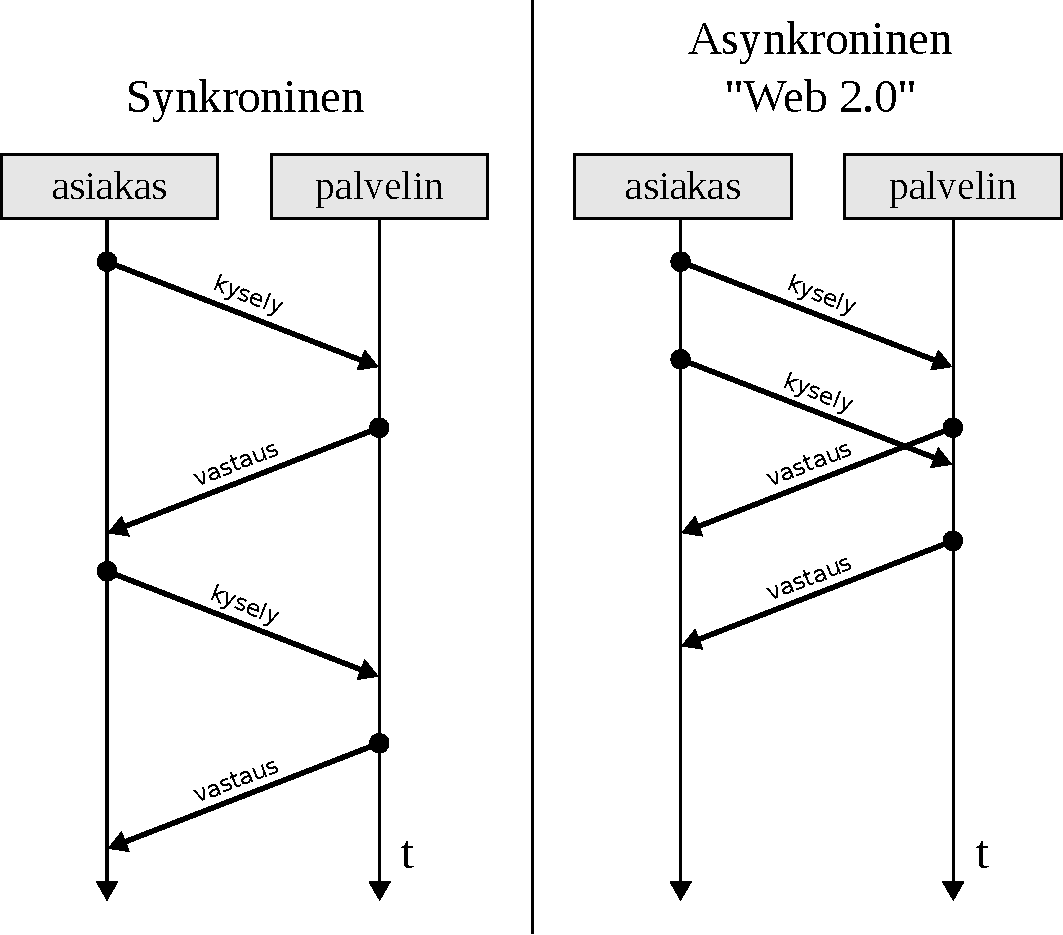
\includegraphics[width=11.5cm]{pics/synkroninen.pdf}
\caption{Synkroninen ja asynkroninen kommunikointi}
\label{synkroninen}
\end{figure}

AJAXiin kohdistuvat hyökkäykset eivät eroa suuresti vanhoista murtautumismenetelmistä. Hyökkääjät pyrkivät edelleen hyödyntämään syötteen puutteellista suodattamista, muokkaamaan 
ulostulevaa dataa, murtamaan salauksia ja hankkimaan istuntonkohtaisia tietoja esimerkiksi evästeitä varastamalla. Hyökkääjien näkökulmasta AJAXin tekee erityisen kiinnostavaksi se,
että aiempaa suurempi osa web-palvelun käyttämästä laskennasta suoritetaan käyttäjän selaimessa. Käyttäjän selaimeen, eli ns. asiakaspuoleen, ei voida kuitenkaan koskaan luottaa.
JavaScriptien huolimaton käyttö avaakin hyökkääjille lukuisia tapoja murtautua palveluihin. Kyseessä on sinänsä pitkään tunnettu ongelma, mutta kehittäjien kiinnostuksen siirtyessä 
AJAXiin ovat myös hyökkääjät alkaneet kiinnittämään asiaan enemmän huomiota \cite{AJAX}. Monet käytetyistä AJAX-ympäristöistä sisältävät myös eriasteisia tietoturvariskejä, joita 
hyökkääjät voivat hyödyntää \cite{JSH}.

\subsection{JavaScript}

JavaScript on Netscapen suunnittelema skriptikieli, joka tunnettiin aluksi nimellä LiveScript. Sun Microsystemsin kehittämän Java-ohjelmointikielen yleistyessä Netscape päättii muuttaa
sen nimen JavaScriptiksi, toivoen sen käytön yleistyvän Javan menestyksen myötä. JavaScriptillä kirjoitetut skriptit sijoitetaan HTML:n \texttt{<script>}-elementin sisään, josta voi 
olla myös viite erilliseen lähdekooditiedostoon. JavaScript vaatii tuen selaimelta, jollainen löytyy miltei jokaisesta web-se\-lai\-mes\-ta, mukaanlukien yleisimmät mobiililaitteet.

JavaScript on tehokas työkalu, joka mahdollistaa monen muun toiminnon ohella muun muassa dynaamisten web-sivujen tekemisen, viestien kirjoittamisen selaimen tilariville, uusien ikkunoiden
avaamisen ja interaktiivisten lomakkeiden luomisen. Skriptien toiminta rajoittuu kuitenkin web-selaimen toimintoihin, eikä sitä käyttäen voida esimerkiksi kirjoittaa levylle ja levyn 
lukeminen rajoittuu pelkästään evästeisiin \cite{JavaScript}. Näistä rajoituksista huolimatta JavaScript mahdollistaa erittäin monipuolisten toimintojen toteuttamisen web-ympäristössä.

Suurin osa web-sivuilla olevista skripteistä toimii siten, että ne ladataan aluksi käyttäjän koneelle, jonka jälkeen ne suoritetaan selaimessa. Skriptit sijaitsevat ja ne suoritetaan 
käyttäjien koneilla, joten toimintaperiaatten selvittäminen ei ole hyökkääjälle vaikeaa. Asiaa pystytään kuitenkin vaikeuttamaan muutamalla eri tavalla. Näistä yksinkertaisin on 
\emph{obfuskointi}, jonka yhteydessä koodista tehdään vaikeasti luettavaa. Aluksi poistetaan kommentointi ja tyhjät rivivälit, seuraava askel on koodin muuttujien ja objektien
uudelleen nimeäminen, jolloin hyökkääjän on vaikeampi päätellä näistä skriptin toimintaperiaate. Nimet voidaan myös muuttaa esimerkiksi binäärikoodiksi. Nämä keinot ovat kuitenkin 
vain hidasteita osaavalle hyökkääjälle \cite{AJAX}. Palvelu tulisikin suunnitella siten, että kaikki luottamuksellisen tiedon käsittely ja käyttäjän syötteen tarkistukset suoritettaisiin
web-palvelimella. Tällöin käyttäjän selaimessa suoritettaisiin ainoastaan sellainen laskenta, joissa käsitellään käyttäjää itseään koskevaa dataa.

Koneelle ladatut skriptit ajetaan oletuksena hyvin rajatussa tilassa, jossa niillä on pääsy vain kyseistä sivun sisältämään dataan tai siihen hyvin läheisesti kuuluviin dokumentteihin. 
JavaScript noudattaa myös  edellisessä luvussa esitettyä \emph{saman alkuperän} periaatetta, joka estää skriptien suorittamisen muista internet-domaineista kuin siitä, josta skripti on
ladattu. Näin vaikeutetaan hyökkäyksen tekemistä käyttäen toiselta sivulta ladattua haitallista skriptiä, jonka avulla voitaisiin esimerkiksi varastaa evästeitä ja urkkia näppäimistön
painallukset.  Aikaisemmin selaimet ovat sallineet joitain poikkeuksia tähän periaatteeseen, mutta tietoturvasyistä nämä on kuitenkin poistettu.

Liian tiukat tietoturvasäännöt eivät 
kuitenkaan toimi nykyaikaisten web-pal\-ve\-lui\-den kanssa, ja tästä syystä \emph{saman alkuperän} periaatetta on mahdollista löysentää. Esimerkiksi ulkoiset linkit, jotka osoittavat toisella
sivustolla olevaan skriptiin, ohittavat \emph{saman alkuperän}, sillä vaikka itse skripti sijaitsee toisella palvelimella niin se lasketaan kuuluvan siihen sivuun, jossa viittaus
lähdekooditiedostoon on.  Näin kutsutulla skriptillä on pääsy sellaisiin evästeisiin ja tiedostoihin, joihin sillä ei välttämättä tarvitsisi olla oikeuksia. Sivustojen ja palveluiden 
käyttäessä resursseja entistä useammasta lähteestä eri palvelimilta, voi tämä aiheuttaa riskitilanteita, jos jonkin lähteen tietoturva on vaarantunut \cite{AJAX}.

\subsection{AJAXiin liittyvät tietoturvariskit}

Koska AJAXin toiminta perustuu hyvin pitkälti JavaScriptin varaan, on itsestään selvää, että hyökkääjät pyrkivät väärinkäyttämään ensisijaisesti JavaScriptin haavoittuvaisuuksia.  
Asiaa ei auta se, että suurin osa sivustoista on jollakin tavalla alttiina XSS-hyökkäyksille \cite{WEB2c} johtuen huonosti toteutetusta syötteen tarkistuksesta. Asetettuja suodatuksia 
pystytään myös kiertämään käyttäen esimerkiksi kuvalinkkejä ja monia HTML-elementtejä, joiden avulla ajettava skripti voidaan hukuttaa muun syötteen joukkoon. Tästä syystä pelkästään 
tiettyjen merkkijonojen suodattaminen ei takaa suojaa JavaScript-pohjaisilta hyökkäyksiltä. Tehokkain ja yksinkertaisin keino onkin poistaa kaikki HTML-elementteihin kuuluvat merkit, 
jolloin esimerkiksi \texttt{<}-merkistä tulee \texttt{\&lt;} ja \texttt{>}-merkistä \texttt{\&gt;}. Monet ympäristöt mahdollistavat myös suoraan HTML-elementtien poistamisen käyttäjien
jättämistä viesteistä \cite{AJAX}. Tälloin esimerkiksi foorumeilla toisten käyttäjien lähettämistä viesteistä saadaan estettyä niiden mahdollisesti sisältämän JavaScript-ohjelmakoodin
suorittaminen.

Kasvaneella JavaScriptin käytöllä on suora vaikutus myös XSS-hyökkäysten yleistymiseen. JavaScriptillä pääsee helposti evästeisiin käsiksi käyttäen \emph{document.cookie}-oliota. 
Vaikka sen käyttö on rajoitettu ainoastaan sen internet-domainin evästeeseen, josta kutsu on tehty, voidaan tämä rajoitus ohittaa melko helposti. Hyökkääjälle riittää, että käyttäjä 
vierailee esimerkiksi sellaisessa foorumissa tai blogissa, joissa käyttäjien viesteissä sallitaan XHTML:n käyttö. Tämä mahdollistaa haitallisten skriptien lähettämisen sivustolle ja pahaa
aavistamaton käyttäjä, joka vierailee tällä sivulla, joutuu tietämättään hyökkäyksen kohteeksi.

Yksi tapa suojautua evästeiden varastamiselta on käyttää HTTP-only~-evästeitä, jolloin asiakaspuolen evästeitä ei pystytä lukemaan. Näiden evästeiden tukeminen on kuitenkin selainkohtaista,
joten tämä ratkaisu ei aina välttämättä ole mahdollista toteuttaa. XSS-hyökkäykset eivät myöskään rajoitu pelkästään evästeiden varastamiseen, ja yhtä helposti hyökkääjä voi esimerkiksi
luoda skriptin, joka lukee näppäimistön painallukset ja lähettää ne haluttuun osoitteeseen. HTTP-only -evästeiden käyttö ei myöskään täysin suojaa evästeitä, jos käytetään XHR-kutsuja. 
Tällöin hyökkääjän on mahdollista lukea suoraan otsaketiedoissa asetettuja arvoja. Jotkut XHR-objekteihin liittyvät haavoittuvuudet ovat myös niin syvällä XHMLHttpRequest-objekteissa, että 
kaikki nykyisin käytössä olevat toteutukset ovat niille jossakin määrin alttiina. Kaapattujen XHR-objektien tunnistaminen ei myöskään vielä ole mahdollista \cite{AJAX}. Näistä syistä johtuen 
AJAX tarjoaa nyt ja tulevaisuudessa hyökkääjille monia mahdollisuuksia murtaa asetettuja suojauksia.

Yksi yleisimmistä AJAXissa käytetyistä dataformaateista on JavaScript Object Notationt (lyh. JSON). Se on ohjelmointikielestä riippumaton ja laajasti tuettu web-palvelimella käytetty 
työkalu. Se on rakenteeltaan hyvin kevyt, ja se koostuu kahdesta eri tietotyypistä: olioista ja taulukoista \cite{JSON}. Formaatin heikkous piilee siinä, että JSON-olio itsessään on kelvollinen 
JavaScript-ohjelma, jonka sisältö on mahdollista kaapata \cite{AJAX}. Termi \emph{JavaScript Hijacking} kuvaa tällaista tilannetta, jossa hyökkääjä ohittaa \emph{saman alkuperän} periaatteen 
silloin, kun JavaScriptiä käytetään arkaluontoisen tiedon lähettämiseen. Aiheesta tehdyn tutkimuksen \cite{JSH} mukaan lähes jokainen käytetty AJAX-ympäristö on alttiina tällaisilla hyökkäyksille.
Käyttäen CSRF-hyökkäystä hyökkääjä pystyy väärinkäyttämään JSON-formaattia, ja varastamaan sekä muokkaamaan toiselle sivustolle lähetettäviä paketteja.  Tälläinen hyökkäys voidaan toteuttaa 
useilla eri tavoilla mukaanlukien käyttäen \texttt{<script>}-elementtiä, ja koska pyyntö tulee selaimen luottamasta lähteestä, voidaan tällä tavoin ohittaa esimerkiksi SSL-suojaus\cite{AJAX}.

Suojautuminen tämän tyyppisiltä hyökkäyksiltä voidaan toteuttaa monella eri tapaa, ja paras tulos saadaan yhdistelemällä näitä. Koska CSRF-hyökkäyksessä hyökkääjä joutuu toimimaan osittain 
sokeasti, voidaan jokaiseen pyyntöön lisätä parametri, jota hyökkääjän on vaikea arvata. Palvelin voidaan myös asettaa tarkistamaan HTTP Referer -kenttä, jolla voidaan varmistaa, että pyyntö 
tulee sallitulta taholta, vaikkakin Referer-kentän sisältö voidaan helposti muuttaa. Toinen tapa on muokata vastaanottopäässä paketteja siten, että hyökkääjä ei pysty ajamaan lähettämissään 
pyynnöissä skriptejä 
\cite{JSH}.

\section{Flash}

AJAXin ohella Macromedian suunnittelema ja nykyisin Adoben kehittämä Flash on ollut yksi niistä merkittävistä tekniikoista, joita käyttämällä YouTuben ja MySpacen kaltaiset 
menestyspalvelut ovat olleet mahdollisia toteuttaa. Flashia käyttämällä kehittäjät ovat jo pitkään pystyneet luomaan interaktiivista ja rikasta web-sisältöä
yksinkertaisista animaatioista aina monimutkaisiin peleihin ja valikoihin asti. Suurin osa web-sivustoilla olevista mainoksista on myös toteutettu käyttäen Flashia. Näistä syistä johtuen 
Flash Player on yksi ohjelmistoalan de facto~-tekniikoista, jonka käyttöaste yritys- ja kuluttajapuolella on lähes 100 prosenttia \cite{Flash}.

Flashin käyttämä ActionScript-skriptikieli muistuttaa läheisesti JavaScriptiä, ja sitä käyttäen on mahdollista luoda uusia TCP-yhteyksiä, ajaa JavaScriptiä selaimessa ja luoda 
sallittuihin domaineihin HTTP-pyyntöjä. Flashin käyttämä tietoturvamalli noudattaa paljolti \emph{saman alkuperän} periaatetta, jolla rajoitetaan eri domaineissa sijaitsevien sovellusten 
kommunikointia. Domainien välinen kommunikointi on kuitenkin sallittua, ja käytetty tietoturvapolitiikka luetaan tähän tarkoitetusta XML-tiedostosta. Tämä XML-tiedosto sijaitsee usein 
domainin juuressa, ja se sisältää ne domainit, jotka saavat olla siihen yhteydessä. Osa Flashiin kohdistuvista hyökkäyksistä pyrkiikin muokkaamaan tietoturvapolitiikkatiedoston sisältöä
siten, että kohde sallisi yhteydet myös hyökkääjän käyttämästä osoitteesta. Tämä voidaan toteuttaa esimerkiksi käyttämällä vihamielistä RSS-syötettä tai luomalla tiedosto, joka sisältää
uuden XML-tiedoston. Yksi tällaisista hyökkäyksistä on Stefan Esserin luoma GIF-tiedosto, jonka kommenttiin on piilotettu uusi tietoturvapolitiikka. Hyökkääjälle riittää, että kohdekone 
vain mahdollistaa tiedoston lataamisen palvelimelle, jonka jälkeen vanha sisältö voidaan korvata GIF-tiedostoon piilotetulla \cite{WEB2}.

Perimmäinen syy sille, miksi XSS-hyökkäykset ovat yleistyneet viime vuosina on se, että käyttäjien antamaa syötettä ei usein tarkisteta riittävällä tarkkuudella. Sama pätee myös suureen 
osaan Flash-pohjaisista toteutuksista, joihin käyttäjien on mahdollista antaa syötteitä. Tämä avaa useita erilaisia Flashia hyödyntäviä XSS-hyökkäyksiä, jotka pyrkivät väärinkäyttämään 
käyttäjän selaimen ja sivuston välistä luottamussuhdetta. Aina vika ei ole Flash-toteutuksen tekijässä, sillä Flash-tiedostoja luodaan usein automaattisesti käyttämällä valmiita 
sovelluksia. Aiheesta tehdyn kattavan tutkimuksen mukaan \cite{FlashXSS} suurimmasta osasta näin luoduista tiedostoista löytyy XSS-haavoittuvaisuuksia, jotka mahdollistavat JavaScriptin
ajamisen siinä domainissa, jossa haavoittuvainen SWF-tiedosto sijaitsee. Osa näistä tietoturvaongelmista on myöhemmin korjattu tutkimuksen julkaisun jälkeen, mutta tehty tutkimus osoittaa 
sen, että edes luotettavina pidettävien tahojen toteutuksiin ei pidä luottaa liikaa.

Yksi käytetyimmistä Flash-pohjaisista toteutuksista ovat erilaiset interaktiiviset mainokset, joita löytyy lähes jokaiselta sivustolta. Flashin levinneisyyden ansiosta ne toimivat miltei
jokaisella käyttäjällä, ja siksi ne ovat houkutteleva keino toteuttaa hyökkäyksiä. Adobe Flash Playerista on löydetty useita eri haavoittuvaisuuksia, jotka ovat mahdollistaneet haitallisten
koodien ajamisen kohdekoneessa. Flash-mainoksia käytetään myös laajalti haittaohjelmien levittämiseen, ja usein tällä tavalla altistuneet koneet kuuluvat käyttäjän tietämättä 
bottiverkkoihin, joita käytetään roskapostin lähettämiseen ja palvelunestohyökkäyksiin. Haitallista koodia sisältävä mainos voi myös esimerkiksi pyrkiä ohjaamaan selaimen toiselle 
sivustolle käyttäen ActionScriptia.  Tällaiset haitalliset mainokset eivät ole pelkästään vain pienten sivustojen ongelma, sillä vuonna 2009 suuret sivustot kuten \emph{guardian.co.uk} 
sisälsivät mainoksia, jotka olivat luonteeltaan haitallisia \cite{FlashAdd}.

\section{Google Web Toolkit}

Nykyisin yhä useampi taho pyrkii hyödyntämään tekniikoita kuten AJAXia ja JavaScriptiä omissa web-palveluissaan, ja tulevaisuudessa tämä kasvu tulee vain jatkumaan. Toimivien ja 
turvallisten  web-palveluiden suunnitteleminen ja toteuttaminen vaatii kuitenkin sellaista syvällistä tietämystä käytetyistä tekniikoista, jota harvemmin suunnittelijoilta löytyy. 
Tämä on yksi  niistä pääsyistä, jonka takia web-pohjaiset hyökkäykset ovat kasvaneet määrällisesti suurimmaksi hyökkäystavaksi. Asian helpottamiseksi on kehitetty erilaisia 
kehitysympäristöjä, jotka pyrkivät helpottamaan suunnittelijoiden taakkaa, ja samalla tarjoamaan jonkinlaista tietoturvaa. Yksi tällaisista on Googlen kehittämä Google Web Toolkit, 
joka on kasvamassa yhdeksi käytetyimmistä kehitysympäristöistä, ja jolla on tehty muun muassa Google Wave ja AdWords.

\subsection{Google Web Toolkit lyhyesti}

Google Web Toolkit (lyh. GWT) on avoimeen lähdekoodiin perustuva kehitysympäristö rikkaiden ja dynaamisten web-sovellusten kehittämiseen. Suunnittelun lähtökohtana on ollut mahdollistaa
korkealaatuisten web-sovellusten tehokas suunnittelu ilman, että kehittäjän tulee olla asiantuntija niin selainten pienissä kummallisuuksissa kuin myös XMLHttpRequest- pyyntöjen
tekemisessä ja JavaScriptien kirjoittamisessa. Tämä on mahdollista, koska GWT:llä AJAX-sovellukset kirjoitetaan Javalla, joka mahdollistaa keskittymisen korkeamman tason suunnitteluun 
ilman, että aikaa tuhlaantuisi DOM- ja XHR-kutsujen säätämiseen. Valmis Java-sovellus käännetään automaattisesti JavaScriptiksi, ja samalla skriptien sisältö optimoidaan muun muassa
poistamalla käyttämättömät muuttuja ja parametrit. Tämän ratkaisun etuna on myös se, että kehittäjät voivat käyttää haluamaansa Java-ympäristöä sovellusten kirjoittamiseen ja koodin 
tarkistamiseen. Käännetyt JavaScriptit myös toimivat suoraan suurimmassa osassa selaimista sekä Androidissa ja iPhonessa \cite{GWT}.

\subsection{Google Web Toolkitin ominaisuuksia}

GWT 2.0 on uusin versio ympäristöstä, ja se on tuonut mukanaan suuren joukon uusia ominaisuuksia vanhoihin versioihin verrattuna. Yksi tärkeimmistä on niin kutsutun ``hosted moden'' 
korvaaminen \emph{GWT Developer} liitännäisellä. Hosted mode oli yksi GWT:een kantavista ideoista, joka mahdollisti tietyn selainympäristön emuloimisen. Hosted modea käyttäen 
kehittäjällä oli mahdollisuus kirjoittaa Java-koodia ja tutkia sen toimivuutta web-selaimessa ilman, että koodia piti kääntää JavaScriptiksi. Tämä säästi reilusti kehittäjän aikaa, sillä 
ison koodin kääntäminen on aina hidasta. Tämän ratkaisun ongelmana oli se, että emuloidut ympäristöt edustivat vanhoja selainversioita, eikä selaimille jo valmiiksi kirjoitettuja 
testausohjelmia kuten Firebugia pystynyt käyttämään. Käyttäen Developer pluginia kehittäjien on nyt mahdollista ajaa ja testata koodia suoraan suosituimmilla selaimilla, jolloin esimerkiksi
tyylitiedostojen säätäminen on helpompaa. Koodin testaaminen yhtäaikaisesti useammalla eri selaimella on myös mahdollista \cite{GWTnew}. 

Toinen suuri uudistus GWT 2.0:ssa on mahdollisuus pilkkoa ajettava koodi pienempiin osiin (Code Splitting). Nykyisten AJAX-sovellusten ongelmana on se, että sivun sisältö pitää lähes aina 
ladata kokonaan selaimeen, ennen kuin palvelua voidaan käyttää. Sivustojen kasvaessa entistä suuremmiksi tämä kasvattaa käyttäjien kokemaa viivettä, ja yksi AJAXin eduista on juuri
viipeen vähentäminen. Pilkkomalla ajettava JavaScripti haluttuihin osiin käyttäen valmista funktiota, voidaan tämä ongelma välttää kokonaan. Riittää, että kehittäjä määrittää ne kohdat, 
jotka hän haluaa ladattavan pienemmissä osissa. Tällä tavoin voidaan esimerkiksi ladata ensiksi käyttöliittymä ja yleisimmin käytetyt valikot, ja vasta käytön aikana ladata vähemmän 
käytetyt toiminnot. GWT pitää myös itse huolen siitä, että kaikki tarvittavat riippuvuudet ladataan oikessa järjestyksessä \cite{GWTnew}

\subsection{Google Web Toolkitin tietoturva}

Koska GWT:n lopputuotos on JavaScriptiä, on se periaatteessa samalla tavalla haavoittuvainen hyökkäyksille kuten Cross-Site Scriptingille ja Cross-Site Request Forgerylle. Yleisellä tasolla 
GWT:een tuottama JavaScripti noudattaa hyväksi todettuja käytäntöjä, jotka vähentävät riskiä joutua tällaisten hyökkäysten kohteeksi. On kuitenkin asioita, joihin kehittäjien tulee edelleen
kiinnittää tarkkaa huomiota. 

Ensimmäinen näistä on olla käyttämättä omia ja kolmannen osapuolen skriptejä sekaisin. Tiettyjen toimintojen kuten innerHTML:n ja eval-funktion kanssa tulee myös olla erittäin tarkkana.
Esimerkiksi innerHTML-atribuuttia käytetään usein staattisen HTML-sisällön tuomiseen JavaScript-objektin määrittämiin valmiisiin taulukoihin ja ikkunoihin. Tämän tekniikan käyttäminen on 
kuitenkin riskialtista, sillä se mahdollistaa haitallisen koodin sisällyttämisen suoraan sivustolle. Mihinkään syötteeseen ei pidä myöskään koskaan luottaa suoraan, vaikka se tulisi omalta 
palvelimelta erityisesti jos se on menossa innerHTML- tai eval-funktioiden käyttöön. Sama pätee myös JSON-syötteisiin, joiden avulla on mahdollista suoraan ajaa haitallista JavaScriptiä, jos 
syötettä ei tarkisteta riittävällä tarkkuudella. Tärkeintä onkin aina tarkistaa erittäin tarkasti eri syötteet riippumatta siitä, mikä osapuoli sen on lähettänyt ja mihinkä käyttöön se on
menossa \cite{GWTsecurity}.

CSRF-hyökkäykset kohdistuvat aina palvelinpuolen huonosti toteutettuun sessionhallintaan, jossa pyynnön tehneen tahon oikeellisuutta ei varmisteta. Määrittämällä JavaScript kopioimaan aina 
sessiossa käytetyn evästeen arvo jokaiseen kyselyyn mukaan, voi palvelin verrata tätä arvoa luomaansa evästeeseen. Koska \emph{saman alkuperän} periaate estää kolmannen osapuolen sivustoa 
pääsemästä käsiksi tähän evästeeseen, voi palvelin olla varma, että pyynnön on todellakin tehnyt käyttäjä itse. GWT:stä löytyy valmiiksi tähän tarkoitukseen kirjoitettuja funktioita, joita
käyttäen jokaiseen pyyntöön voidaan lisätä oikean evästeen arvo. Näitä käyttäen CSRF-hyökkäykset voidaan lähes kokonaan poistaa, kunhan vain palvelinpuoli osaa verrata evästeiden arvoja 
ja tehdä näiden pohjalta oikeat johtopäätökset. JSONin tapauksessa voidaan tämän lisäksi käyttää jo aikaisemmin esitettyä tapaa, jossa pakettien sisältöä muokataan siten, ettei niiden
sisältöä voida kaapata käyttäen <script>-elementtiä \cite{GWTsecurity}.


% -*- mode: LaTeX; coding: utf-8; -*-

\chapter{Aiheeseen liittyvä tutkimus}

\section{Yleistä}

Viime vuosina web-sovellukset ovat kasvattaneet suuresti suosiota, ja nykyisin yhä useampi palvelu, jossa tietoturvan ja saatavuuden takaaminen on elintärkeää, on siirtynyt osittain tai kokonaan 
verkon puolelle. Tämä on vaikuttanut suuresti siihen, mihin tietoturvahyökkäykset nykyisin kohdistuvat, ja kuinka niitä pyritään toteuttamaan. Hyökkäysten muuttuessa yhä hienostuneimmiksi, 
eivät perinteiset tietoturvamenetelmät enää riitä suojaamaan loppukäyttäjiä tai palvelun ylläpitäjiä. Tästä syystä erilaisten tietoturvaratkaisuiden ympärillä käy kova kuhina, ja aihepiiri 
on herättänyt suurta kiinnostusta tutkijoiden keskuudessa. Erilaisia ratkaisuja, joissa on pyritty selvittämään aikaisemmissa luvuissa esitettyjä tietoturvahyökkäyksiä ja näiden 
mukana tulleita haasteita, on lukematon määrä. Seuraavaksi esitellyt tutkimukset edustavat vain pientä osaa koko tutkimuskentästä, mutta jo näistä käy ilmi se, millaisia ratkaisumalleja
nykyisin etsitään.

Hyökkäysten tunnistaminen toimii siten, että analysoimalla yhtä tai useampaa tapahtumaa pyritään löytämään viitteitä tapahtuvista hyökkäyksistä. Tunnistamiseen pohjautuvat menetelmät jaetaan usein
kahteen eri tyyppiin: anomalioiden eli poikkeavuuksien tunnistamiseen (eng. anomaly detection) ja väärinkäytösten tunnistamiseen (eng. misuse detection). Näistä anomalioiden tunnistamiseen perustuvat
järjestelmät luovat malleja järjestelmän, käyttäjän tai verkon normaalista käyttäytymisestä, ja vertaamalla tapahtumia näin muodostettuihin kuvauksiin, voidaan poikkeavuudet tunnistaa. Väärinkäytösten 
tunnistamiseen tarkoitetut järjestelmät taas sisältävät joukon kuvauksia eli signatuureja tunnetuista hyökkäyksistä. Tuleva liikenne tarkistetaan näitä kuvauksia vastaan, jolloin kuvauksia vastaavat
hyökkäykset voidaan tunnistaa. Joissakin tapauksissa jaottelu on myös tehty sen mukaan, mistä tutkittava liikenne on kerätty. Tällöin järjestelmät on jaettu verkkoon pohjautuviksi (eng. network based)
ja asiakaspohjaisiksi (eng. host based). 

\section{Väärinkäytösten tunnistaminen}

Väärinkäytökseen perustuvat järjestelmät ovat pitkään olleet suosituin lähestymistapa hyökkäysten torjumiseen. Nämä järjestelmät on voitu jakaa kahteen erilliseen osaan, jossa tilattomassa 
järjestelmässä jokaista tulevaa tapahtumaa käsitellään itsenäisesti, kun taas tilallisessa järjestelmässä tutkitaan tapahtumien välisiä suhteita. Web-pohjaisten hyökkäysten tutkimisessa tietolähteinä 
on käytetty mm. palvelimien tuottamaa lokia \cite{LightTool}, ja IDS-järjestelmien \cite{Snort}\cite{Bro} tapauksessa analysoimalla verkkokerroksen liikennettä. Ensimmäisessä ratkaisussa ongelmana
on, että itse palvelimiin kohdistuvia hyökkäyksiä ei pystytä havaitsemaan ainoastaan lokitietoa tarkkailemalla. Samoin hyökkäyksiä, jotka koostuvat monista eri vaiheesta, on mahdotonta mallintaa. 
Verkkokerroksella toimivia järjestelmiä taas pystytään harhauttamaan muokkaamalla hyökkäyksiä, ja näistä harvat mahdollistavat tilallisen analyysin. 

Esitettyjä ongelmia on pyritty ratkaisemaan lisäämällä havaittavien tapahtumien määrää, ja keräämällä informaatiota eri lähteistä. Esimerkiksi asentamalla sovellustasolle erillinen tiedonkeruuseen 
tarkoitettu komponentti \cite{Application} on saatu hyviä tuloksia. Tässä tapauksessa tiedonkeruu tapahtui Apache-palvelimelle asennetun komponentin välityksellä, joka tarkkaile lokitiedon lisäksi
mm. pyyntöjen tulkitsemiseen ja toteuttamiseen menevää aikaa. Tämän ratkaisun etuna on myös se, että tutkittava data on salaamattomassa muodossa, ja sessioiden uudelleenrakentaminen on mahdollista. 
Tällä tasolla toimiva IDS-järjestelmä voi myös toimia ennaltaehkäisevästi eli haitalliseksi havaittu liikenne voidaan tiputtaa pois ennen kuin se käsitellään palvelimella. Suurimpana haittapuolena on, 
että tietylle sovellukselle suunniteltua komponenttia ei voida sellaisenaan käyttää muilla alustoilla. 

WebSTAT \cite{Webstat} on tilalliseen analyysiin perustuva IDS-järjestelmä, joka pohjautuu STAT-kehitysympäristöön \cite{STAT}. WebSTAT hyödyntää STATL-ohjelmointikieltä, joka mahdollistaa hyökkäysten
mallintamisen ottamalla huomioon mm. eri tapahtumien välisiä yhteyksiä ja verkkohistoriaa sekä palvelimien kuten Apachen ja Microsoftin IIS:n lokia. Koska tietoa kerätään yhtäaikaisesti monesta eri 
lähteestä, voidaan palvelimien lokitiedon analysointiin yhdistää alempien toimintojen kuten jär\-jes\-tel\-mä- ja verkkotason tuottamaa tietoa. Näin tehty analyysi kuvaa koko järjestelmä tilaa, jolloin 
yllättävät muutokset pystytään havaitsemaan nopeasti. Testien mukaan tällainen analyysi voidaan toteuttaa suurissa järjestelmissä reaaliajassa aiheuttamatta suurempaa viivettä palvelimien toiminnassa. 
Menetelmän sovittaminen tiettyyn järjestelmään vaatii jonkin verran manuaalista työtä, ja tätä voidaankin pitää sen suurimpana heikkoutena. Monimutkaisten hyökkäysten kuvaaminen on usein myös hankala
toteuttaa, ja niiden tulkitsemiseen saattaa tuhlaantua turhaa aikaa.

Väärinkäytösten tunnistamiseen tarkoitettuja järjestelmiä on hyödynnetty myös uudempien tietoturvahyökkäysten tunnistamisessa. Esimerkiksi vihamielisten Flash-mainosten tunnistamiseen tarkoitettu 
OdoSwiff \cite{FlashAdd} pyrkii etsimään sivuilla olevista mainoksista hyökkäykseen tarkoitettua koodia käyttäen staattista ja dynaamista analyysia. Palvelinpuolella XSS-hyökkäyksiä vastaan on luotu 
järjestelmä, josta löytyy yleisimpien hyökkäysten kuvaukset \cite{SignatureXSS}. Kumpikin järjestelmistä toimii erittäin hyvin, kunhan hyökkäys on entuudestaan tuttu.

\section{Poikkeavuuksien tunnistaminen}

Väärinkäytösten tunnistamiseen käytettyjen järjestelmien suurin heikkous piilee siinä, että mallintamattomat hyökkäykset jäävät näiltä huomaamatta. Tämä on erityisesti web-palveluihin kohdistuvien
hyökkäysten tapauksessa iso ongelma, sillä toimintaympäristö muuttuu jatkuvasti, ja uusia hyökkäyksiä ja vanhojena variaatioita ilmestyy tiuhaan tahtiin. Tällöin signatuurien pitäminen ajantasalla
muodostuu mahdottomaksi tehtäväksi. Hyökkäysten monimuotoisuus onkin johtanut siihen, että nykyisin yhä useammassa järjestelmässä pyritään tunnistamaan poikkeavat tapahtumat normaaliin liikenteen seasta
ilman tarkkoja signatuureja. 

Anomalioiden tunnistamiseen on käytössä useita eri menetelmiä, ja ne voidaan jakaa kahteen eri ryhmään \cite{State}. Näistä ensimmäinen sisältää oppimiseen pohjautuvat mallit, jossa normaali 
käyttäytyminen opetetaan opetusmateriaalin avulla. Normaalia käyttäytymistä esittävät profiilit voidaan mallintaa käyttäen joko sään\-tö\-poh\-jais\-ta-, mallipohjaista- tai tilastopohjaista menetelmää. Näistä
sääntöpohjaiset menetelmät muistuttavat eniten perinteisiä IDS-järjestelmiä sillä erolla, että luodut säännöt pohjautuvat kerättävään dataan, ja säännöt voivat olla rakenteiltaan hyvin monimutkaisia. 
Mallipohjaisissa menetelmissä taas luodaan normaalia käyttäytymistä kuvaavat profiilit, jota vastaan tuleva liikenne arvioidaan. Tiedonlouhinta, neuroverkot ja liikenteestä luotujen kuvioiden vertaaminen
tulevaan liikenteeseen (eng. pattern matching) ovat tekniikoita, joita on käytetty tällaisten mallien luomiseen. Analyysissa voidaan esimerkiksi tutkia verkkopakettien kuormia \cite{Payload}\cite{ULISSE} 
ja klusteroimalla ja luokittelemalla liikenne protokollien ja palveluiden mukaan \cite{Cluster}. Viimeisen ryhmän muodostavat tilastollisiin menetelmiin pohjautuvat menetelmät \cite{PacketHeader}, jotka
ovat jääneet vähemmälle huomiolle johtuen alati muuttuvasta toimintaympäristöstä.

Toisen ryhmä anomalioiden tutkimisessa muodostavat spesifistiset mallit (eng. spesification model). Nämä menetelmät pohjautuvat enemmän ihmisten huomioihin ja asiantuntijuuteen kuin matemaattisiin
kuvauksiin. Menetelmissä käytetään useita eri elementtejä aina sovellustasolta verkkotasolle, ja näitä käyttäen luodaan normaalia käyttäytymistä kuvaavat mallit. Järjestelmät voivat hyödyntää esimerkiksi
protokollista kerättävää tietoa anomalioiden tunnistamisessa. Järjestelmien eri tiloja ja tapahtumien välisiä suhteita voidaan myös mallintaa, jolloin poikkeavat tilat ja tapahtumaketjut voidaan
tunnistaa. 

Anomalioiden tunnistamiseen perustuville järjestelmille löytyy useita eri käyttökohteita. Niillä voidaan esimerkiksi pyrkiä tunnistamaan tietokantoihin kohdistuvia tunnettuja ja tuntemattomia SQL-hyökkäyksiä.
Järjestelmälle voidaan opettaa normaali käyttäytyminen esimerkiksi tiedonlouhintamenetelmin \cite{Data} tai luomalla profiileja normaalista käyttäytymisestä \cite{SQLanomaly}\cite{SQLlearning}. Erilaisia
menetelmiä voidaan myös yhdistellä, jolloin todennäköisyys poikkeavan liikenteen tunnistamiseen kasvaa. Tutkimalla esimerkiksi yhtä aikaisesti sekä web-pyynnöissä että SQL-kyselyissä ilmeneviä poikkeavuuksia, 
voidaan tulevat kyselyt pisteyttää tarkasti \cite{WebSQL}. Kyselyiden kategoriointi mahdollistaa sen, että haitalliseksikin merkityt kyselyt voidaan ohjata sellaisille palvelimille, joilla ei ole 
pääsyä arkaluontoiseen tietoon. 

Web-palveluihin kohdistuvien hyökkäysten tunnistaminen on hankala ja aikaa vievä prosessi. Aikaisemmin tässä työssä esitetyt hyökkäykset kattavat vain osan hyökkäyksistä, joita vastaan sovellussuunnittelijat ja
ylläpitäjät joutuvat suojautumaan. Juuri tämä hyökkäysten monimuotoisuus on se seikka, joka on nostanut anomaliatutkimuksen muiden menetelmien yläpuolelle, ja aihepiiri on viime vuosina noussut yhdeksi 
puhutuimmista tietoturvan saralla. 

Poikkeavan tilan tunnistamiseen on käytetty monia eri menetelmiä, ja päätöksen tekemiseen on käytetty useita eri tietolähteitä. Esimerkiksi Swaddler \cite{Swaddler} on 
web-sovelluksille suunniteltu menetelmä, joka oppii kriittisten järjestelmäkutsujen ja sovelluksen tilojen väliset suhteen analysoimalla web-sovelluksen sisäisiä tiloja. Tällä tavoin voidaan tunnistaa hyökkäykset,
jotka aiheuttavat poikkeavia tiloja esimerkiksi sovelluksen normaaliin työkulkuun. Järjestelmä koostuu eri malleista ja osista, joille opetetaan harjoittelujakson aikana sitä vastaava normaali käytös. Jokaiselle
osalle, jotka käytännössä vastaavat tiettyjä sovelluksen toimintoja, lasketaan myös kynnysarvo, jonka ylittyessä sen aiheuttanut toiminto lasketaan anomaliaksi. Tehdyissä testeissä järjestelmä tunnisti 
kaikki toteutetut hyökkäykset, ja virheellisten positiivisten hälystysten määrä oli kohtuullisen pieni. Analysointi aiheutti jonkin verran kuormaa palvelimelle, mutta optimoimalla toteutusta tämä voidaan poistaa
lähes kokonaan. 

Aikaisemmin esitettyä tapaa, jossa hyödynnetään palvelimen tuottamaa logia, voidaan käyttää myös poikkeavuuksien tunnistamisessa \cite{Multi}. Tässä tapauksessa analysoitiin Apachen tuottamaa HTTP-logia, ja huomio kiinnitettiin kyselyihin, joissa parametreja käyttäen välitettiin arvoja palvelinpuolen ohjelmille tai aktivoitiin dokumentteja. Kyselyt purettiin osiin, ja niitä analysoitiin käyttäen useita eri malleja 
mm. kyselyjen pituutta ja normaalia järjestystä, merkkien jakaumia ja pyyntöjen tiheyttä. Vastaavaa mallia on sovellettu myös poikkeavien järjestelmäkutsujen tunnistamisessa \cite{SystemCall}, joten sen käyttö ei rajoitu pelkästään web-palveluihin. Väärinkäytös- ja anomaliamenetelmien yhdistämistä on myös ehdotettu \cite{Combination}. Tällainen järjestelmä voi toimia siten, että tuleva liikenne syötetään ensiksi anomalioita tutkivalle järjestelmälle, ja vain tunnistetut positiiviset tapaukset ohjataan väärinkäytösjärjestelmälle. Menetelmän etuna on, että virheellisten positiivisten määrä tippuu suuresti, ja tarkan analyysin vaativat tapahtumat pienenevät.



% -*- mode: LaTeX; coding: utf-8; -*-

\chapter{Tutkimuksessa käytetyt menetelmät}

Edellisissä luvuissa on esitetty osa niistä hyökkäyksistä, joita vastaan verkot ja Web-palvelut joutuvat nykyisin suojautumaan. Niiden suuresta määrästä johtuen on ilmiselvää, että täysin 
turvallista ympäristöä on mahdoton rakentaa. Tätä ei edes pidetä tietoturvasuunnittelun lähtökohtana, vaan tärkeämpää on löytää tasapaino palvelun saatavuuden ja käytettyjen tietoturvaratkaisuiden 
välillä. Liian raskaat menetelmät aiheuttavat ylimääräistä viivettä palvelun tai verkon saatavuuteen, ja liian kevyet ratkaisut jättävät ne avoimiksi tietoturvahyökkäyksille. 

Ongelmia lokin analysoimisessa aiheuttaa aineiston suuri määrä, ja siinä esiintyvien parametrien tyypit. Parametreista osa on luokka-asteikollisia ja osa puolestaan numeroasteikollisia, joten tietynlaisten toimintamallien 
etsiminen näistä suoraan on haastavaa. Parametrien suuri määrä aiheuttaa myös laskennallisia ongelmia, joten niiden määrää tulee pystyä jotenkin vähentämään säilyttäen kuitenkin mahdollisimman tarkkaan alkuperäisten
muuttujien piirteet. Seuraavaksi esitellään yleisellä tasolla analysoinnissa käytetyt tekniikat, ja tätä seuraa näiden tarkempi matemaattinen kuvaus.


\section{Menetelmien yleinen kuvaus}
 
Anomalioiden tunnistamiseen käyttämämme järjestelmä pohjautuu diffuusiokuvausten ja diffuusioetäisyyksien käyttöön. Ne tarjoavat tehokkaan tavan löytää merkittäviä geometrisia rakenteita datasta, ja niiden
käyttämistä moniulotteisen datan esittämisessä on esitelty \cite{diff} \cite{diff2}. Menetelmien tehokkuus perustuu siihen, että diffuusiokuvausten avulla pystytään vähentämään analysoitavan datan dimensioita
säilyttäen kuitenkin sen rakenne. Periaatteessa dimensioiden vähentäminen tarkoittaa sitä, että datajoukko esitetään toisella datajoukolla, jonka dimensio on pienempi. Tällöin sen klusteroiminen sekä 
analysoiminen ja esittäminen graafisesti on helpompaa.

Datan luonteesta johtuen pelkkä dimensioiden vähentäminen ei tuo esille poikkeavuuksia, vaan tätä varten tarvitaan parametreja, jotka kuvaavat HTTP-pyynnön sisältöä tarkemmin. Suurimmasta osasta kyselyn
sisältämistä parametreista kuten IP-osoitteesta, ajasta tai käytetystä selaimesta tämä ei käy ilmi. Toki näistä voidaan tunnistaa esimerkiksi hyökkäykset, joissa yritetään kuluttaa palvelimen resurssit loppuun
hakemalla samaa resurssia yhä uudestaan tai pommittamalla uusia yhteysyrityksiä. Web-palveluihin kohdistuvat hyökkäykset ovat kuitenkin usein paljon hienovaraisempia. Parhaiten näitä voidaan yrittää tunnistaa
tutkimalla tarkemmin GET-parametrin jälkeistä osaa, josta käy ilmi parametrit, joita hyökkääjä välittää palvelimelle. 

Dimensioiden vähentäminen tapahtuu laskemalla diffuusioetäisyydet eli keskimääräiset arvot kaikista kahden pisteen välisistä poluista ts. todennäköisyydet kulkea satunnaiskululla pisteestä toiseen kiinteällä
askelmäärällä. Ennen tätä analysoitava data tulee muuttaa kategoriseksi, sillä muuten erilaisten parametrityyppien välisiä etäisyyksiä ei pystyä laskemaan. Osa parametreista on jo valmiiksi kategorisessa 
muodossa, mutta numeerinen data tulee erikseen kategorisoida. Numeerisen datan automaattinen kategorisointi tapahtuu klusteroimalla yhtä ominaisuutta, ja laskemalla klusteroinnin hyvyysarvo. Tätä jatketaan niin pitkään,
kunnes optimaalinen klusterointi on saavutettu. Prosessi toistetaan vaihtaen kategorioiden lukumäärää jokaisessa iteraatiossa, ja se luku, joka tuottaa parhaimman arvon, valitaan optimaaliseksi kategorioiden 
määräksi .

Tietoturvahyökkäyksissä hyökkääjä pyrkii aina ohittamaan jollakin tavalla asetetut suojaukset. Usein tämä tarkoittaa sitä, että palvelimelle välitetyt pyynnöt muodostuvat pitkistä merkkijonoista, ja niissä käytetyt
merkit poikkeavat tyypillisesti käytetyistä merkeistä. Useiden peräkkäisten avain-arvo parien määrä myös saattaa kasvaa reilusti tavallista suuremmaksi. Näiden tunnistamista varten käytämme analyysissa n-gram -analyysiksi
kutsuttua menetelmää. Menetelmällä lasketaan datassa esiintyvien peräkkäisten merkkien tai sanasten esiintyvyystiheyksiä. Analyysi voidaan tehdä esimerkiksi koko kyselylle, avain-arvo -pareille tai avainten nimille. 

Suurilla tietomassoilla n-gram -analyysi tuottaa isoja matriiseja, joiden käsitteleminen on hidasta. Tehokkuuden takia matriisien ulottuvuuksia tulee pystyä jollakin tavalla vähentämään. Tämä onnistuu satunnaisprojektion 
avulla, joka on ulottuvuuksien vähentämiseen tarkoitettu menetelmä. Satunnaisprojektiossa moniulotteinen data heijastetaan pienempiulotteiseen aliavaruuteen käyttäen satunnaisesti luotua matriisia. Näin syntynyt uusi 
matriisi on laskennallisesti tehokas, ja se säilyttää tässä tapauksessa riittävän määrän informaatiota. 

\section{Diffuusiokuvaus}

Moniulotteisen datan analysoiminen on aina haasteellinen tehtävä johtuen parametrien suuresta määrästä. Tämän takia käytämme tässä työssä hyödyksi diffuusiokuvauksia, jotka ovat tehokas tapa vähentää analysoitavan datan
ulottuvuuksia säilyttäen kuitenkin sen rakenne. Tämän jälkeen esimerkiksi klusterointi ja visualisointi pienempiulotteisessa avaruudessa on helpompaa.

Ensimmäiseksi diffuusiokuvausiin perustuvalle järjestelmälle opetetaan datan normaali käyttätyminen. Tämä tapahtuu käyttäen opetusmateriaalia, joka on osa analysoitavaa dataa. Olkoot tämä opetusmateriaali 
$\Gamma = \left\{ x_1, x_2, \dots , x_N \right\}, x_i \in \mathbb{R}^n$, jossa $N$ on kyselyiden määrä ja $n$ alkuperäisen datan ulottuvuuksien määrä. Meidän tapauksessamme data muodostaa $N \times n$ matriisin, jossa 
rivit pitävät sisällään yksittäiset kyselyt, ja sarakkeet ovat näiden analysoitavat parametrit.

Aluksi luomme samankaltaisuusmatriisin, joka kuvaa eri pisteiden välisiä etäisyyksiä. Naapuruston laajuuden määrittää euklidinen etäisyys $\epsilon$, jonka arvona voidaan käyttää haluttua mittaa. Tutkimuksessamme käytämme arvona painotettua Hammingin etäisyyttä.

\begin{equation}
W_{ij} = e^{-\frac{||x_i - x_j||^2}{\epsilon}}
\label{KERNEL}
\end{equation}

Näin luodun matriisin rivit normalisoidaan diagonaalimatriisin $D$ avulla, joka luodaan yhtälössä \ref{ROWSUM}. 

\begin{equation}
D_{ii} = \sum_{j=1}^{N} W_{ij}
\label{ROWSUM}
\end{equation}

Nyt jokaisen rivin summaksi tulee 1. Tätä todennäköisyyttä siirtyä datapisteestä toiseen kuvatkoon $P$

\begin{equation}
P = D^{-1} W
\label{PROB}
\end{equation}

$P$:n ominaisvektorit ovat samat kuin konjugaattimatriisin, joka on esitetty yhtälössä \ref{SYMM}. 

\begin{equation}
\tilde{P} = D^{\frac{1}{2}} P D^{-\frac{1}{2}}
\label{SYMM}
\end{equation}

Jos vaihdamme $P$:n yhtälöstä \ref{SYMM} yhtälössä \ref{PROB} olevan kanssa, saamme yhtälön \ref{NGL} todennäköisyysmatriisin $\tilde{P}$. Näin luotua matriisia kutsutaan normalisoiduksi graafin  Laplace-operaatioksi.

\begin{equation}
\tilde{P} = D^{\frac{1}{2}} P D^{-\frac{1}{2}} = D^{\frac{1}{2}} D^{-1} W D^{-\frac{1}{2}} = D^{-\frac{1}{2}} W D^{-\frac{1}{2}}
\label{NGL}
\end{equation}

Tämän jälkeen symmetrinen matriisi hajoitetaan käyttäen singulaarihajotelmaa (engl. Singular Value Decomposition = SVD). Koska $\tilde{P}$ on normaalimatriisi, spektraaliteorian (spectral theorem) mukaan tällaisen matriisin 
hajotelma on yhtälön \ref{SVD} mukainen.  

\begin{equation}
\tilde{P} = U \Lambda U^*
\label{SVD}
\end{equation}

Matriisissa $\Lambda$ diagonaalilla olevat singlulaariarvot vastaavat matriisissa $\tilde{P}$ olevia ominaisarvoja, koska se on symmetrinen. Edelleen koska $\tilde{P}$ on konjugaatti $P$:n kanssa, sisältävät nämä kaksi samat ominaisarvot. 

Matriisin $U = [ u_0, u_1, \dots, u_k ]$ sarakkeet sisältävät matriisin $\tilde{P}$ $k$ ominaisvektoria $u_k$. Käyttämällä yhtälöä \ref{EIGENVECTORS}, voime laskea matriisin $P$ oikeat ominaisvektorit $v_k$, jolloin 
saamme ne matriisin $V$ sarakkeina  $V = [v_0, v_1, \dots, v_k]$.  

\begin{equation}
V = D^{-\frac{1}{2}} U
\label{EIGENVECTORS}
\end{equation}

Nyt datan koordinaatit pienennetyssä ulottuvuudessa ovat yhtälön \ref{MAP_COORDINATES} matriisissa $\Psi$. 

\begin{equation}
\Psi = V \Lambda
\label{MAP_COORDINATES}
\end{equation}

Käyttämällä sopivaa arvoa $\epsilon$ lähestyvät ominaisarvot nopeasti nollaa, jolloin riittävän tarkkaan diffuusiokuvaukseen tarvitaan ainoastaan $d$ komponenttia. Ensimmäinen ominaisvektori $v_0$ on vakio, joten se voidaan jättää pois.
Käyttäen ainoastaan ensimmäiset $d$ komponenttia diffuusiokuvauksen luomiseen on esitetty yhtälössä \ref{DM}.

\begin{equation}
\Psi_d : x_i \to \left[ \lambda_1 V_{i1}, \lambda_2 V_{i2}, \dots, \lambda_d V_{id} \right]
\label{DM}
\end{equation}

Tämä diffuusiokuvaus upottaa tunnetut pisteet $x_i$ $d$-ulotteiseen avaruuteen. Näin ollen datan uusi ulottuvuus on $d$ vanhan $n$ sijaan.

\section{$N$-gram -analyysi}

Koska haluamme analysoida tarkemmin GET-parametrin jälkeistä kyselyosuutta, tarvitsemme tähän menetelmän, joka toimii nopeasti ja tehokkaasti. $N$-gram -analyysi on hyvin tunnettu ja käytetty menetelmä, jolla tutkitaan 
peräkkäisten merkkien tai sanasten esiintymistiheyttä. Sitä käytetään laajalti muun muassa tilastollisen kielen analyysissa, jossa esimerkiksi puheentunnistuksessa sillä tutkitaan foneemeja eli kielen äänneyksikköjä. 

Meidän tapauksessa tutkittavat yksiköt ovat merkkejä, joiden esiintymistiheyttä ja jakaantumista analysoidaan. Merkkien $n$-gram lasketaan käyttäen $n$ pituista liukuvaa ikkunaa. Esimerkiksi sanan ``automaatti'' 2-gram 
saadaan aloittamalla analyysi ensimmäisestä kirjaimesta ja liuttumalla ikkunaa yhden kirjaimen verran. Tässä tapauksessa syntynyt merkkijakauma on ``au'', ``ut'', ``to'', ``om'', ``ma'', ``aa'', ``at'', ``tt'', ``ti''. 
Käyttäen tällä tavoin syntynyttä sarjaa saadaan rakennettua matriisi, joka sisältää tiedon merkkien jakaantumisesta.

$N$-gram -analyysin tuottamien matriisien ulottuvuus on $m^n$, jossa $m$ on datassa esiintyvien sanasten määrä ja $n$ on n-gram -sarjan pituus. Tutkimuksessa analysoidaan vain kahden peräkkäisen merkin esiintyvyyksiä, 
jolloin $n=2$, ja koska tutkittavat sanaset ovat 8-bittisiä merkkejä, niin $m=2^8=256$. Ulottuvuuksia pystytään vähentämään jonkin verran poistamalla sellaiset ulottuvuudet, joissa jokaisessa vektorissa esiintyisi vain 
nollia. Tästäkin huolimatta matriisit ovat niin moniulotteisia, että ulottuvuuksien määrä tulee pystyä jollakin tavoin vähentämään. 

\section{Satunnaisprojektio}

Satunnaisprojektiossa alkuperäinen $N$-ulotteinen data heijastetaan $k$-ulotteiseen $(k \ll N)$ aliavaruuteen käyttäen satunnaista $k \times N$ matriisia $R$ \cite{Random}. Olkoot meillä esimerkiksi matriisi 
$X_{m\times N}$, jossa $m$ on havaintojen määrä, ja $N$ on datan alkuperäinen dimensio. Olkoot  $k$  sitten uusi haluttu dimensioiden määrä. Uuden matriisin laskemiseksi luodaan satunnainen matriisi 
$R_{n \times k}$, jossa jokaisen sarakkeen arvot ovat satunnaisesti jakautuneet. Kertomalla nämä keskenään saadaan matriisi $X_{m \times k}^{RP}$, joka on esitys alkuperäisestä datasta $X$ heijastettuna $k$-ulotteiseen 
aliavaruuteen:

\begin{equation}
X_{m \times k}^{RP} = X_{m \times N} \cdot R_{n \times k}.
\label{RP}
\end{equation}

Satunnaisprojektion idea on lähtöisin Johnson-Lindenstrauss lemmasta: jos vektoriavaruudessa olevat pisteet heijastetaan satunnaisesti valittuun aliavaruuteen jossa on sopiva määrä ulottuvuuksia, säilyvät pisteiden
väliset etäisyydet riittävällä tarkkuudella. $X_{m \times N} \cdot R_{n \times k}.$ laskemisen aikavaativuus on $O(dkN)$, ja jos matriisi $X$ sisältää pääasiallisesti nollia ja rivissä on keskimääräisesti $c$ kappaletta arvoja 
$(c \ll N)$, on aikavaativuus $O(ckN)$.

Satunnaisesti luotu matriisi $R$ voidaan valita monella eri tapaa. Useimmiten matriisin $R$ elementit $r_{ij}$ noudattavat Gaussin jakaumaa, mutta se voidaan muodostaa myös muulla tavoin kuten esimerkiksi

\begin{equation}
r_{ij} = \sqrt{3}\cdot 
\begin{cases}
 +1 &\text{todennäköisyydellä $\frac{1}{6}$} \\
 0 &\text{todennäköisyydellä $\frac{2}{3}$} \\
 -1 &\text{todennäköisyydellä $\frac{1}{6}$} \\
\end{cases}
\label{RPChoice}
\end{equation}

Tällaisen jakauman käyttäminen vähentää entisestään laskenta-aikaa, sillä laskenta voidaan suorittaa käyttäen kokonaislukuja. Yllä olevan jakauman tapauksessa laskenta on vieläkin nopeampaa, sillä operaatioista
tarvitaan vain kolmasosa, sillä luotu matriisi sisältää suurimmaksi osaksi nollia \cite{Random}.

% -*- mode: LaTeX; coding: utf-8; -*-

\chapter{Tiedon keruu}

TODO.

% -*- mode: LaTeX; coding: utf-8; -*-

\chapter{Analyysi}

Tässä luvussa käydään vaiheittain läpi yhden valitun palvelun analysointi sekä esitetään perustelut, joiden pohjalta tehtyihin ratkaisuihin on päädytty. 
Luvussa myös esitellään analysoinnista saatuja tuloksia sekä pohditaan näihin johtaneita syitä. Lopuksi vielä esitetään jatkotutkimuksen kannalta 
tärkeitä kehitysideoita, joita syntyi tutkimuksen aikana. 
 
\section{Tutkimuksen toteutus}

Saamamme materiaali koostui neljästä eri Web-palvelusta, joista analyysiin valitsimme yhden. Muista palveluista saadut lokitiedostot käsiteltiin
myös valmiiksi, mutta koska lokitietoja oli määrällisesti niin paljon, päädyimme tarkastelemaan tarkemmin vain yhtä. Valitsemastamme palvelusta
analysoimme myös vain viikon mittaisen jakson. Tähän ratkaisuun päädyttiin sen takia, että analysoitavaa dataa oli kerätty noin puolen vuoden ajalta,
joten jo yhden palvelun osalta koko datan läpikäymiseen olisi mennyt kohtuuttomasti aikaa. Käytetyn menetelmän rajoitukset, jotka on kerrottu luvussa \ref{sec:matlab},
asettivat myös käytännön rajoituksia analysoitavien tiedostojen määrälle. Tämän kokoinen otanta oli kuitenkin riittävän suuri esikäsittelijän toimivuuden
testaamiseen, jonka lisäksi käytettyjen menetelmien sopivuutta käytössä olleen materiaalin analysoimiseen voitiin arvioida. 

Esikäsittelyvaiheessa HTTP-kyselyt jaetaan palvelun resurssien mukaan
omiin tiedostoihin, joissa ne ovat CSV-formaatissa kuvan ???
mukaisesti.  Resursseihin kohdistuvien kyselyiden lukumäärä vaihtelee
suuresti sen mukaan, kuinka käytetty mikäkin resurssi on. Web-sivun
ollessa kyseessä lukumäärä vastaa sivun käyntimäärää. Mikäli resurssia
käytetään esimerkiksi muun sivun osana, kuten tyylitiedostojen ja
kuvien tapauksessa, tämä kasvattaa merkittävästi kyselyiden lukumäärää
verrattuna tavanomaiseen Web-sivuun.

Analyysissä käyttämämme viikon pituinen jakso sisälsi yhteensä 913 eri
resurssia ja näihin kohdistuvat kyselymäärät vaihtelivat muutamasta
kappaleesta aina kymmeniin tuhansiin. Koska Web-palveluihin kohdistuvat 
tietoturvahyökkäyksissä hyödynnetään erityisesti HTTP-kyselyn parametriosan 
käsittelyn haavoittuvaisuuksia,keskityimme vain sellaisiin palveluihin, joissa 
esiintyi vaihteleva kirjo parametreja. Tämä rajaus tehtiin suodattamalla pois sellaiset
resurssit, joihin kohdistui alle sata kyselyä ja joiden
GET-parametreistä muodostettujen erilaisten n-grammien määrä oli alle
kymmenen. Suodatuksen jälkeen analysoitavaksi jäi 36
resurssia. Suodatus suoritettiin esikäsitelyn jälkeen ja
suodatusrajat on säädettävissä tiedostosta
\texttt{src/InterestingParameters.hs}.

Käytetyimmissä resursseissa HTTP-kyselyitä oli kymmeniä tuhansia,
joten jokaisesta resurssista ei pystytty suoraan tekemään
diffuusiokuvausta johtuen menetelmän rajoituksista. Ongelma
ratkaistiin valitsemalla satunnaisotannalla ilman takaisinpanoa 2~000
HTTP-kyselyä niistä resursseista, joissa oli kyselyitä yli tämän
määrän. Näin ollen jokaisesta resurssista muodostettiin lopulta
tiedosto, jossa oli enintään 2~000 HTTP-kyselyä.

\begin{figure}[hb]
\centering
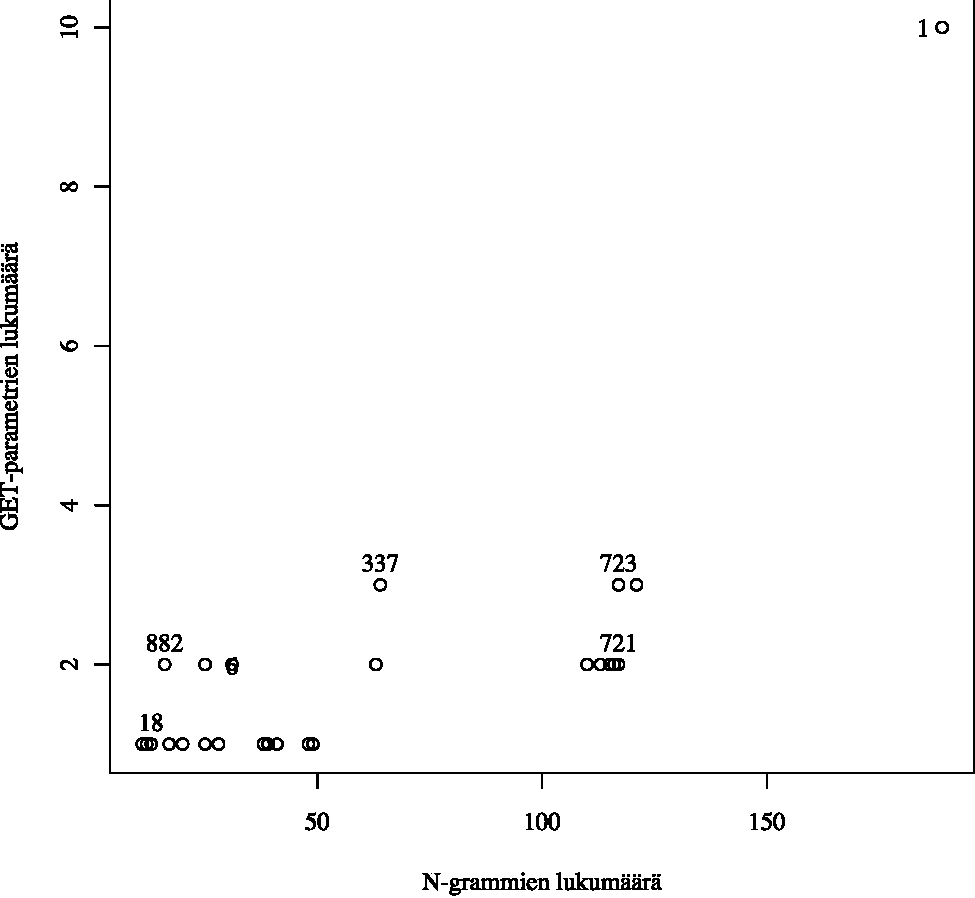
\includegraphics[width=13cm]{pics/service_resources.pdf}
\caption{Palvelun resurssien ominaisuudet.}
\label{service_resources}
\end{figure}

Analysoitavan palvelun eri resurssit on esitetty kuvassa
\ref{service_resources}. Kuvassa vaaka-\-akselina on käytetty
N-grammien lukumäärää ja pystyakselina GET-parametrien
lukumäärää. Resursseista valitsimme kuusi tarkempaan tarkasteluun ja
ne on merkitty kuvaajaan niiden resurssinumerolla.  Resurssit pyrimme
valitsemaan siten, että jokaisesta ryppäästä olisi yksi valittuna.

Palvelun jokaisesta resurssista muodostettiin aluksi diffuusiokuvaus
käyttäen edellä kuvatulla tavalla suodatettua aineistoa.
Analysoimalla saatua diffuusiokuvausta voitiin määrittää ne pisteet,
jotka oli luokiteltu poikkeaviksi siinä joukossa, jossa kyseisiä
pisteitä oli verrattu. 

Seuraavaksi lasketuista diffuusiokuvauksista muodostettiin
diffuusiokartta käytäen toista ja kolmatta ominaisvektoria. Koska
suuri määrä pisteitä sijoittui täsmälleen samoihin koordinaatteihin,
kartan luettavuuden parantamiseksi sirontakuvion pisteitä
``täristettiin''. Täristäminen suoritettiin lisäämällä
ominaisvektorien arvoihin normaalijakaumasta satunnaisesti poimittu
arvo. Normaalijakauman keskihajontana käytettiin yhtä prosenttia
akselin leveydestä. Kuvassa \ref{diffusio_1} nähdään edellä kuvatulla
tavalla muodostettu diffuusiokartta resurssista 1. Kuvaajasta voidaan
havaita, että muutamaa poikkeusta lukuunottamatta pisteet sijoittuivat
hyvin lähelle toisia.

Diffuusiokartta ei ole sellaisenaan kovinkaan havainnollinen, joten
jokaiselle pisteelle laskettiin vielä poikkeavuusluku. Se muodostettiin
summaamalla euklidinen etäisyys lähimpään kolmeen pisteeseen
diffuusiokuvauksen toisen, kolmannen ja neljännen ominaisvektorin
muodostamassa diffuusioavaruudessa. Tämän etäisyystiedon avulla voitiin piste
luokitella poikkeavuudeksi sekä piirtää poikkeavuuskartta.

% FIXME etäisyyskartta -> poikkeavuuskartta. Tuomon vinkki.

Kuvassa \ref{service_1} on resurssista 1 muodostettu poikkeavuuskartta. Kuvaajassa vaaka-akselille on sijoitettu resurssille kohdistuneet HTTP-kyselyt
ja pystyakselin mittana on poikkeavuus. Tässä pystyakseli ilmaisee sen kuinka poikkeava kukin piste on vertailujoukon sisällä. Jokaiselle kuvaajalle
on vielä määritetty keskihajonta ja raja-arvo, jonka ylittäneet pisteet merkitään poikkeaviksi. Tämä raja-arvo vaihtelee tapauskohtaisesti ja sen
arvo on kolme kertaa keskihajonta. Keskihajonta on merkitty kuvaajaan katkoviivalla ja raja-arvo yhtenäisellä viivalla. Esimerkiksi resurssin 1 
poikkeavuusskartassa \ref{service_1} on nähtävissä viisi poikkeavuudeksi merkittyä pistettä.

Jokainen diffuusiokartan luomiseen käytetytty piste pystytään
palauttamaan siihen HTTP-kyselyyn, josta se on
muodostettu. Esitetyissä kuvaajissa palauttamiseen tarvittavat tiedot
on merkitty niihin pisteisiin, jotka ylittävät raja-arvon. Otetaan
esimerkiksi kuvaajan \ref{service_18} ainoaksi merkitty poikkeama,
jolla on arvot ovat 7,3 ja 14594. Näistä ensimmäinen arvo ilmoittaa
sen tiedoston järjestysnumeron, josta kyseinen HTTP-kysely
löytyy. Seuraava luku puolestaan kertoo sen palvelimen
järjestysnumeron, johon kysely on ohjattu. Näiden kahden luvun avulla
voidaan yksilöidä tietty lokitiedosto. Viimeisin luku sisältää
rivinumeron kyseisen lokitiedoston sisällä.

\section{Tulokset}

Analysoitavassa materiaalissa resurssilla 1 \ref{service_1} oli viisi HTTP-kyselyä, jotka merkittiin poikkeaviksi. Tutkimalla diffuusiokuvauksen
luomiseen käytettyä lokia, ja palauttamalla HTTP-kyselyt alkuperäiseen muotoon, pystyimme paikallistamaan nämä kyselyt ja vertaamaan niitä lokin
muihin kyselyihin. Resurssin 1 tapauksessa kolme poikkeavaksi merkittyä kyselyä sisälsi sellaisen tunnistetiedon käyttäjistä, jota ei esiintynyt 
muissa kyselyissä. Kahdesta jäljelle jääneestä kyselystä yhdessä oli yritetty suoraan pyytää sellaista sivustoa, johon palvelu ei todennäköisesti
tarjonnut mahdollisuutta. Viimeisin kysely sitten... FIXME: Tarkistettava Joelilta onko tuossa joku bugi?

Kuvassa \ref{service_18} on nähtävillä resurssin 8 poikkeavuuskartta. Kyseisessä otannassa oli mukana 181 pistettä ja näistä yksi todettiin poikkeavaksi.
Resurssi 8 tarjosi vain staattista sisältöä, joten GET-parametrin jälkeistä kyselyosuutta ei HTTP-kyselyissä pitänyt olla. Poikkeavassa kyselyssä oli
GET-parametrin resurssipolun jälkeen kuitenkin kysymysmerkki, ja tämän perässä oli pyynnön tehneen alustan verkko-osoite. Poikkeavan kyselyn tunnistaminen
oli helppoa, sillä se oli ainoa kysely, jolle n-gram analyysi tuotti rivejä. Resurssille tehty kysely oli selkeästi virheellinen, sillä merkitty verkko-osoite 
oli privaattiverkon osoite. Kyselyssä käytetty alusta oli myös ainoa laatuaan.

Resurssisa 337 \ref{service_337} poikkeavuuksia havaittiin kuusi kappaletta. Näistä neljässä oli GET-parametrin jälkeen lisättynä samanlainen tunnistetieto
kuin resurssin 1 kolmessa havaitussa poikkeavuudessa. Yksi poikkeavuus taas oli saman käyttäjän aiheuttama kuin resurssilla 8, sillä kysely tuli samasta
verkko-osoitteesta ja näiden välillä ei ollut kuin muutama minuutti aikaa. Käytetty alusta oli myös ainoa laatuaan ja kyselyyn oli lisätty perään
sama verkko-osoite. Onkin hyvin todennäköistä, että pyydetyt palvelut eivät ole suunniteltu kyseiselle alustalle, jolloin kyselyiden oikeassa muodostuksessa ilmenee
virheitä. Viimeisessä poikkeavassa kyselyssä oli sitten muista eroava määrä avain-arvo pareja.

Kuvien \ref{service_721} ja \ref{service_723} poikkeavuudet aiheutuivat samaan tapaan ylimääräisestä tunnistetiedosta, joka oli lisätty kyselyiden perään. Kyselyt olivat selkeästi tulleet
saman välityspalvelun kautta, ja niistä jokainen oli tullut eri käyttäjältä. Tämä viittaisikin siihen, että kyseinen välityspalvelu olisi konfiguroitu virheellisesti. Tämän takia
sen kautta tulevat pyynnöt muodostettiin virheellisesti ja palvelimelle tulevia pyyntöjä ei pystytty käsittelemään oikein. Viimeisessä kuvassa \ref{service_882} resurssin poikkeama aiheutui siitä, 
että kyseinen HTTP-pyyntö oli ainoa, johon oli lisätty erillinen arvo. Muut käyttäjät ainoastaan latasivat saman tiedostoa ilman ylimääräisiä parametreja.. 

\begin{figure}[p]
\centering
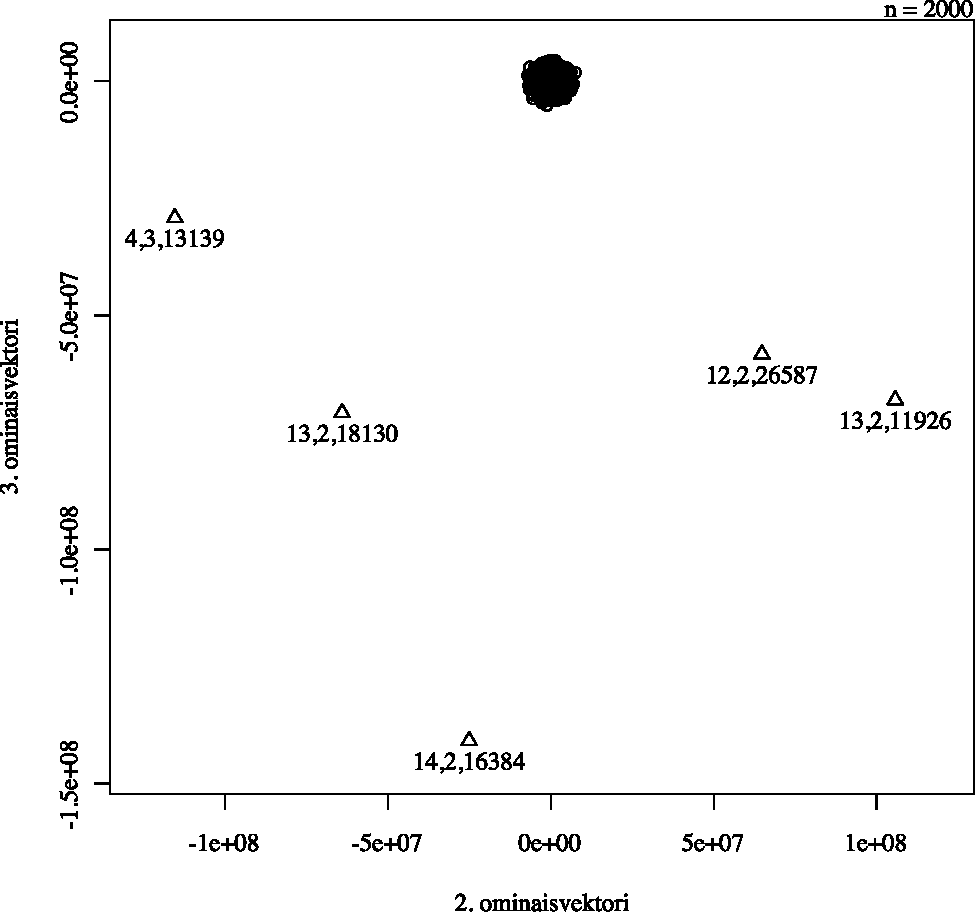
\includegraphics[width=11cm]{pics/diffuusiokuvat/service_1.pdf}
\caption{Resurssin 1 täristetty diffuusiokartta.}
\label{diffusio_1}
\end{figure}

\begin{figure}[p]
\centering
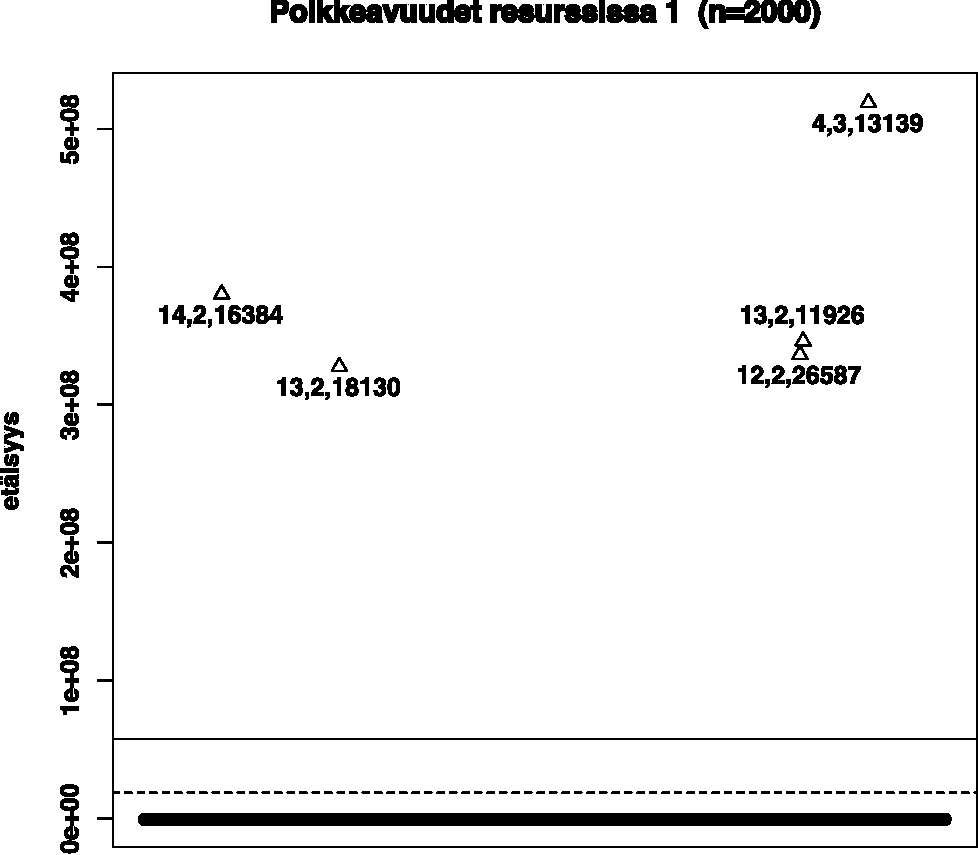
\includegraphics[width=11cm]{pics/tiheyskuvat/service_1.pdf}
\caption{Resurssin 1 poikkeavuuskartta.}
\label{service_1}
\end{figure}

\begin{figure}[p]
\centering
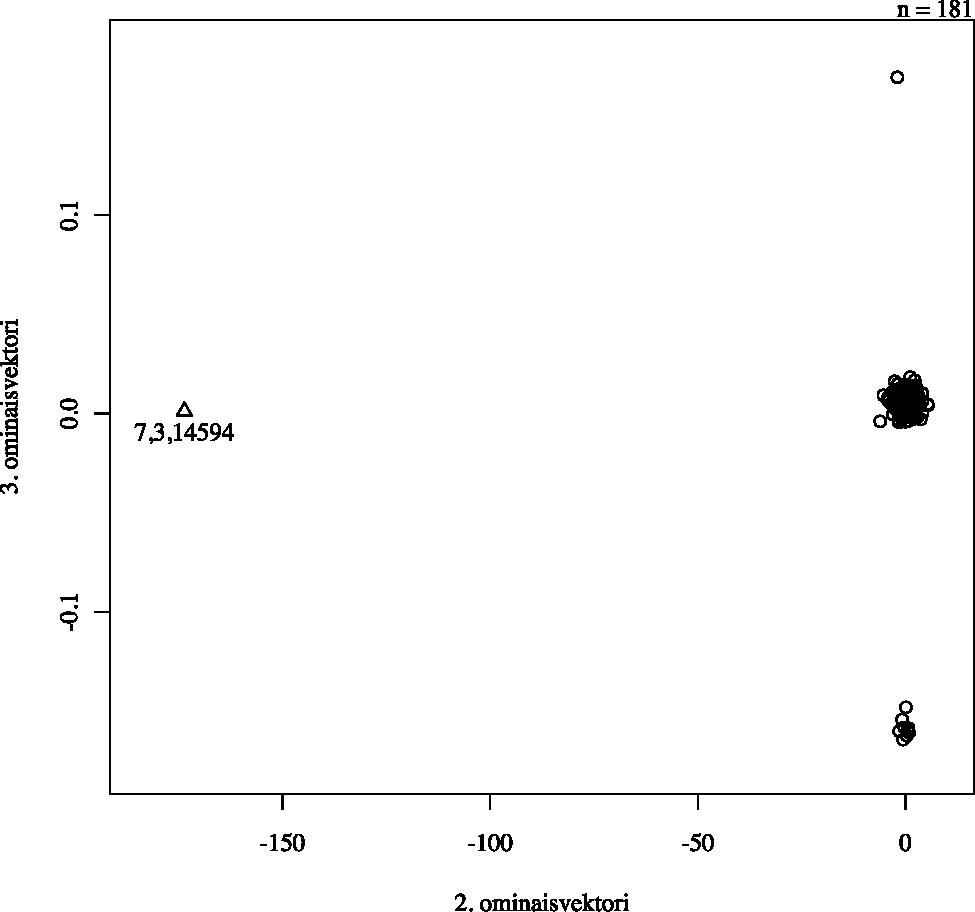
\includegraphics[width=11cm]{pics/diffuusiokuvat/service_18.pdf}
\caption{Resurssin 18 täristetty diffuusiokartta.}
\label{diffusio_18}
\end{figure}

\begin{figure}[p]
\centering
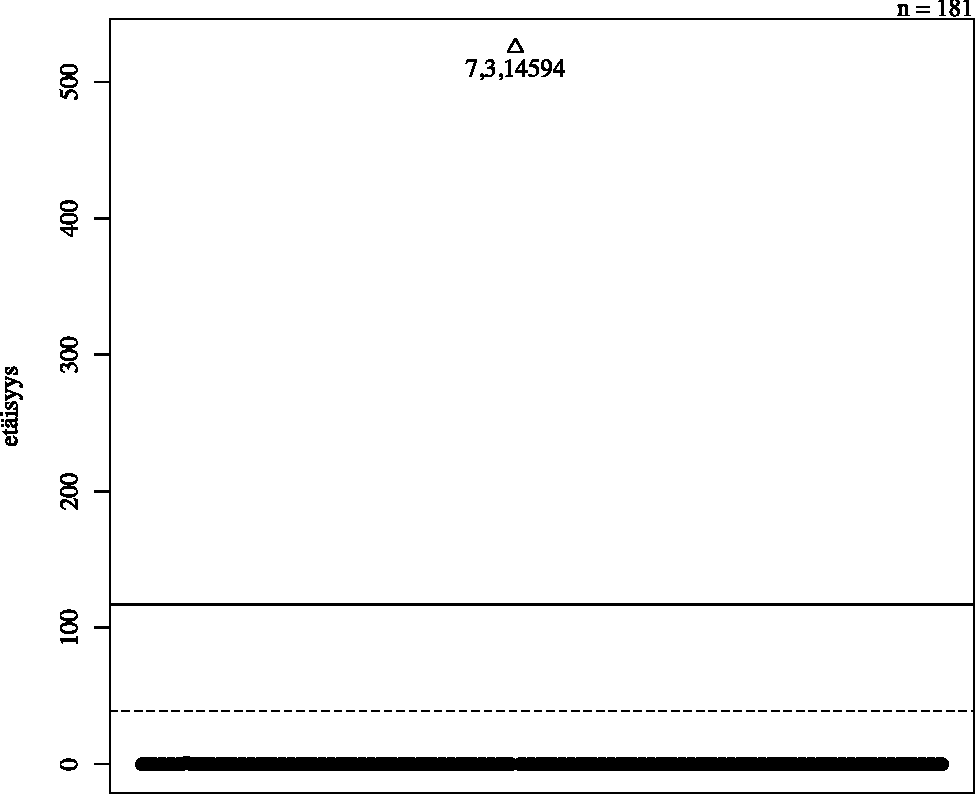
\includegraphics[width=11cm]{pics/tiheyskuvat/service_18.pdf}
\caption{Resurssin 18 poikkeavuuskartta.}
\label{service_18}
\end{figure}

\begin{figure}[p]
\centering
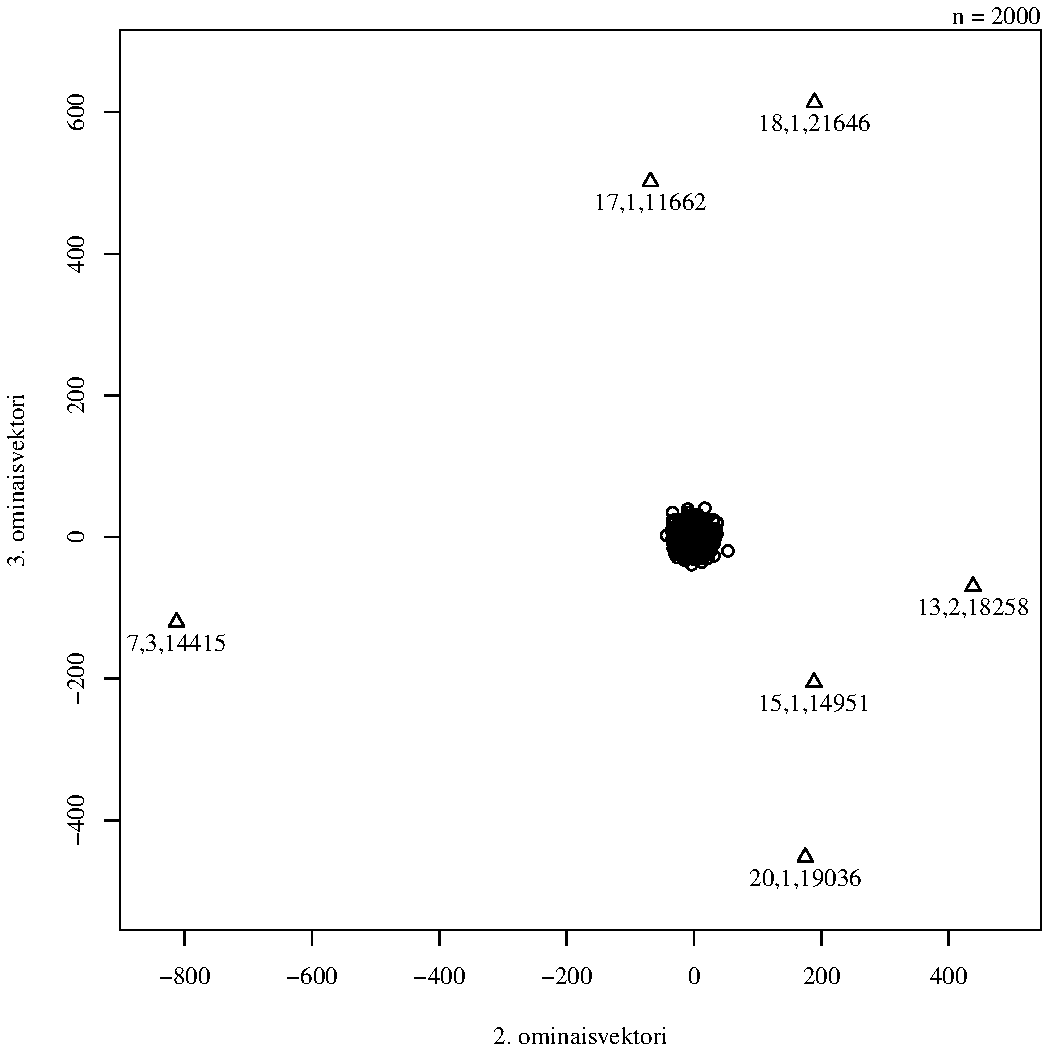
\includegraphics[width=11cm]{pics/diffuusiokuvat/service_337.pdf}
\caption{Resurssin 337 täristetty diffuusiokartta.}
\label{diffusio_337}
\end{figure}

\begin{figure}[p]
\centering
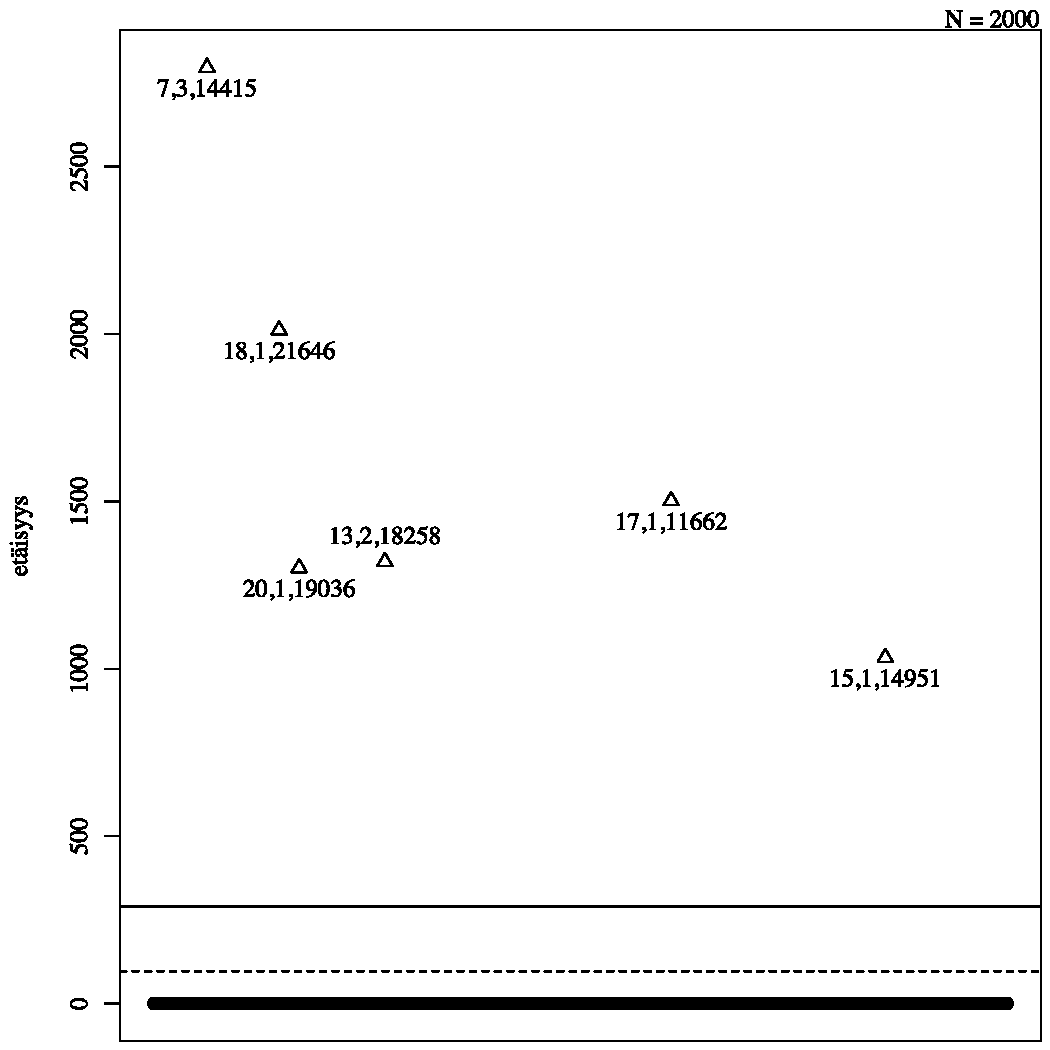
\includegraphics[width=11cm]{pics/tiheyskuvat/service_337.pdf}
\caption{Resurssin 337 poikkeavuuskartta.}
\label{service_337}
\end{figure}

\begin{figure}[p]
\centering
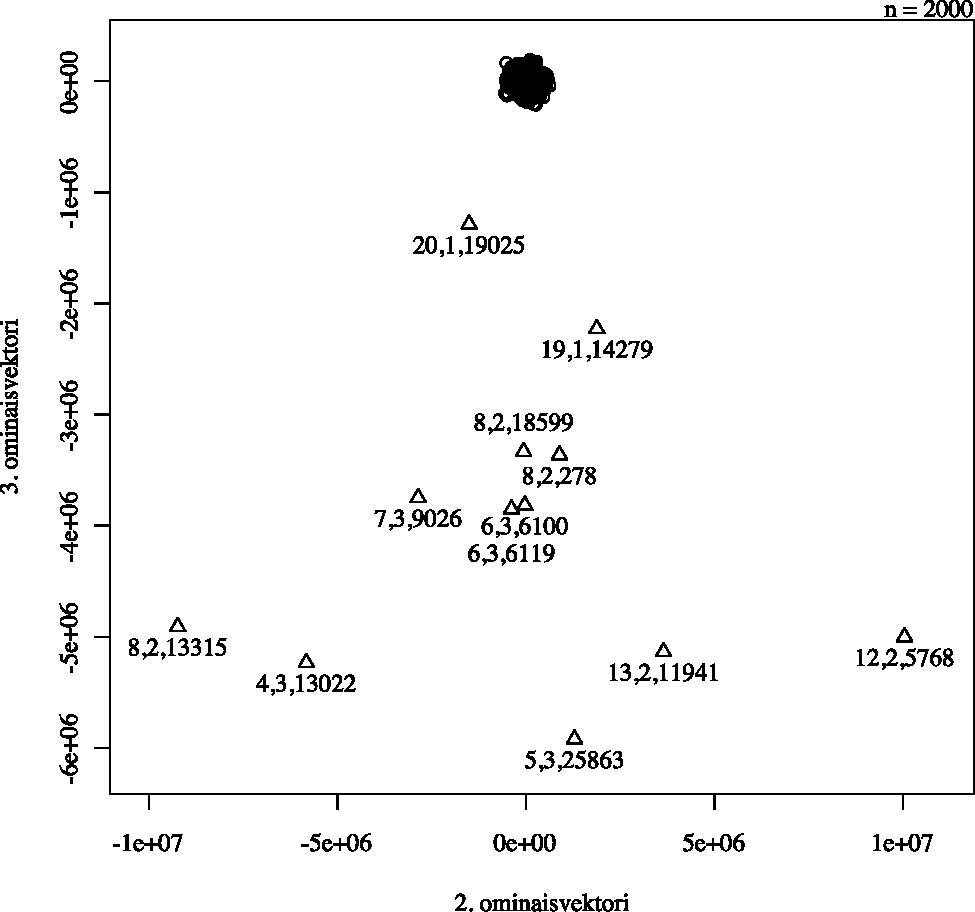
\includegraphics[width=11cm]{pics/diffuusiokuvat/service_721.pdf}
\caption{Resurssin 721 täristetty diffuusiokartta.}
\label{diffusio_721}
\end{figure}

\begin{figure}[p]
\centering
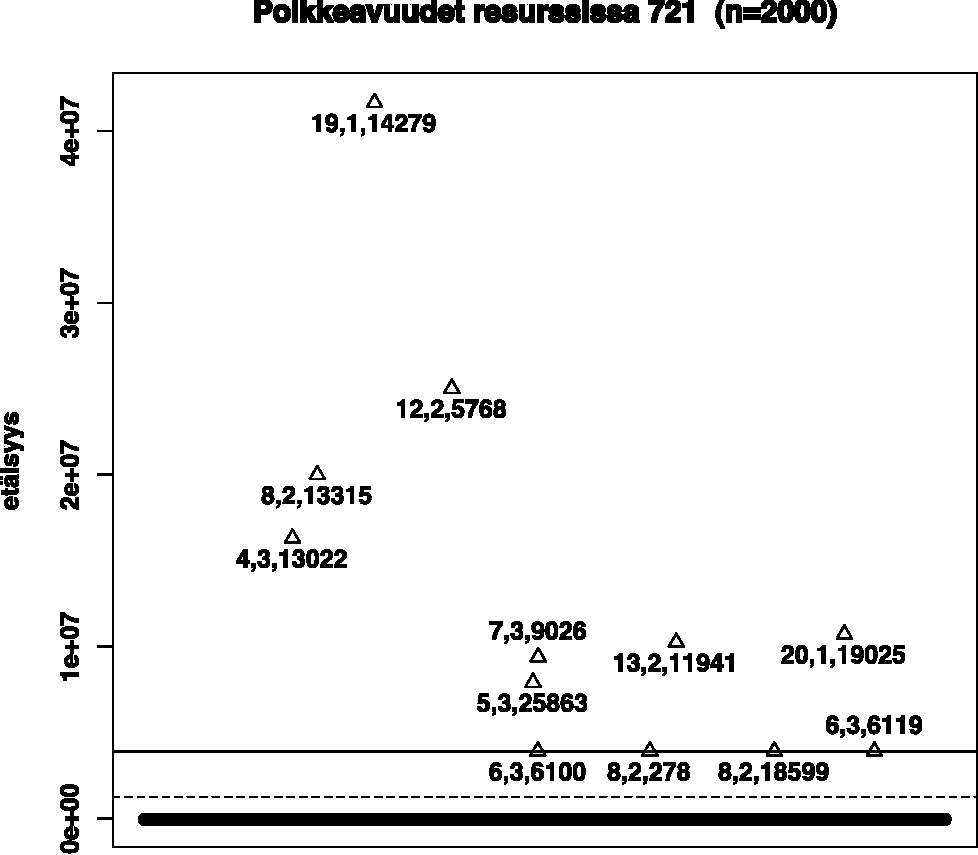
\includegraphics[width=11cm]{pics/tiheyskuvat/service_721.pdf}
\caption{Resurssin 721 poikkeavuuskartta.}
\label{service_721}
\end{figure}

\begin{figure}[p]
\centering
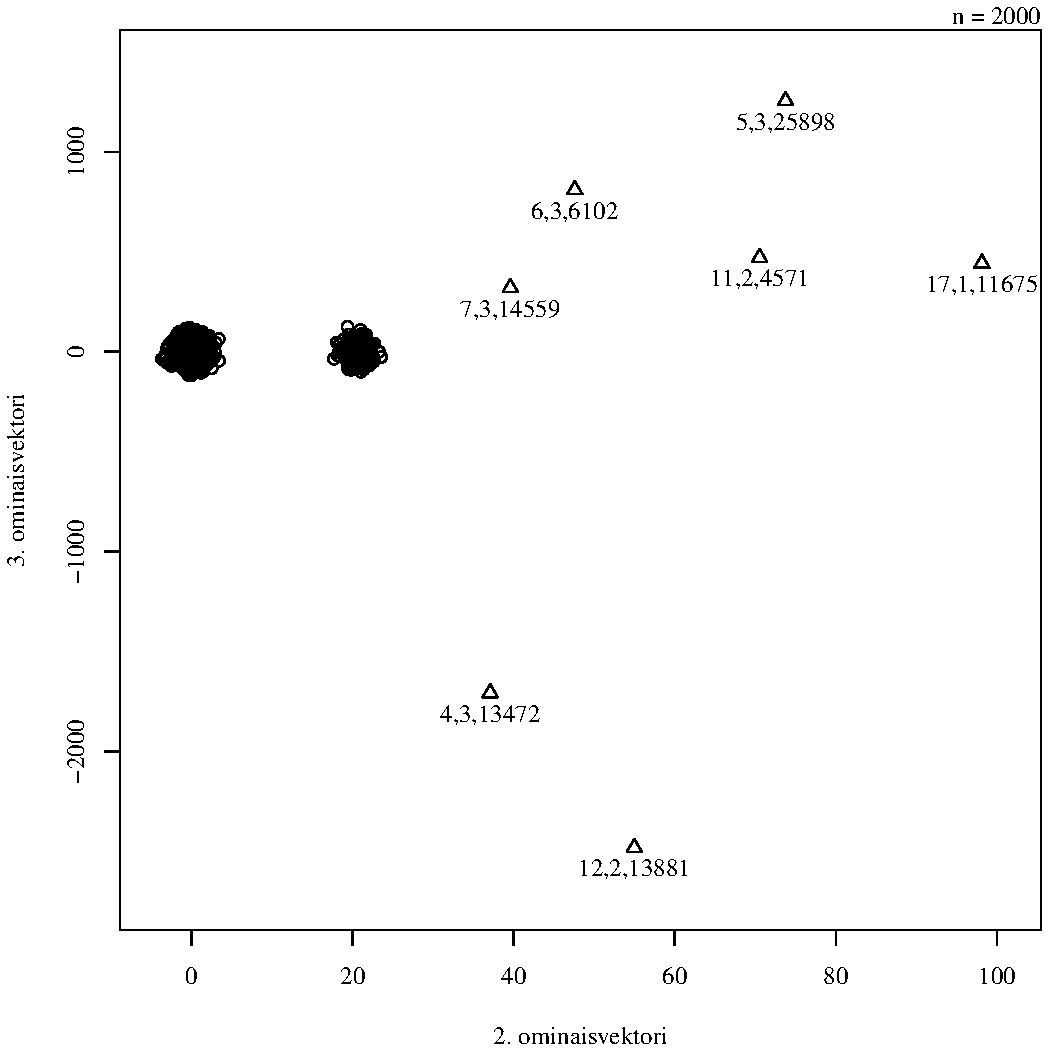
\includegraphics[width=11cm]{pics/diffuusiokuvat/service_723.pdf}
\caption{Resurssin 723 täristetty diffuusiokartta.}
\label{diffusio_723}
\end{figure}

\begin{figure}[p]
\centering
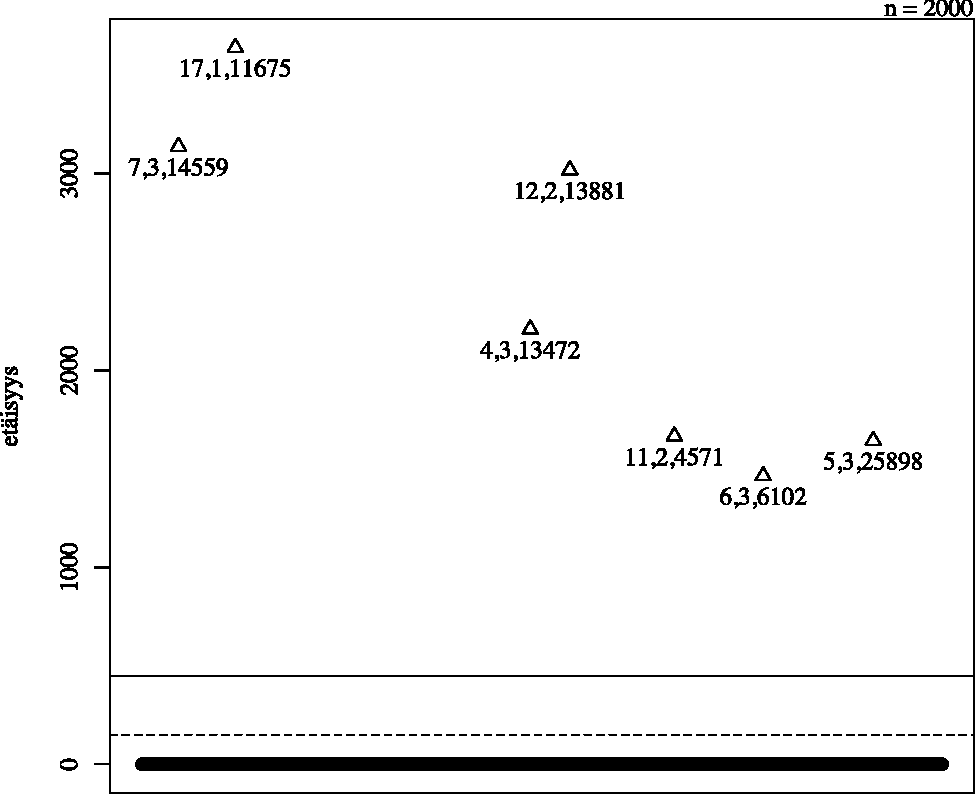
\includegraphics[width=11cm]{pics/tiheyskuvat/service_723.pdf}
\caption{Resurssin 723 poikkeavuuskartta.}
\label{service_723}
\end{figure}

\begin{figure}[p]
\centering
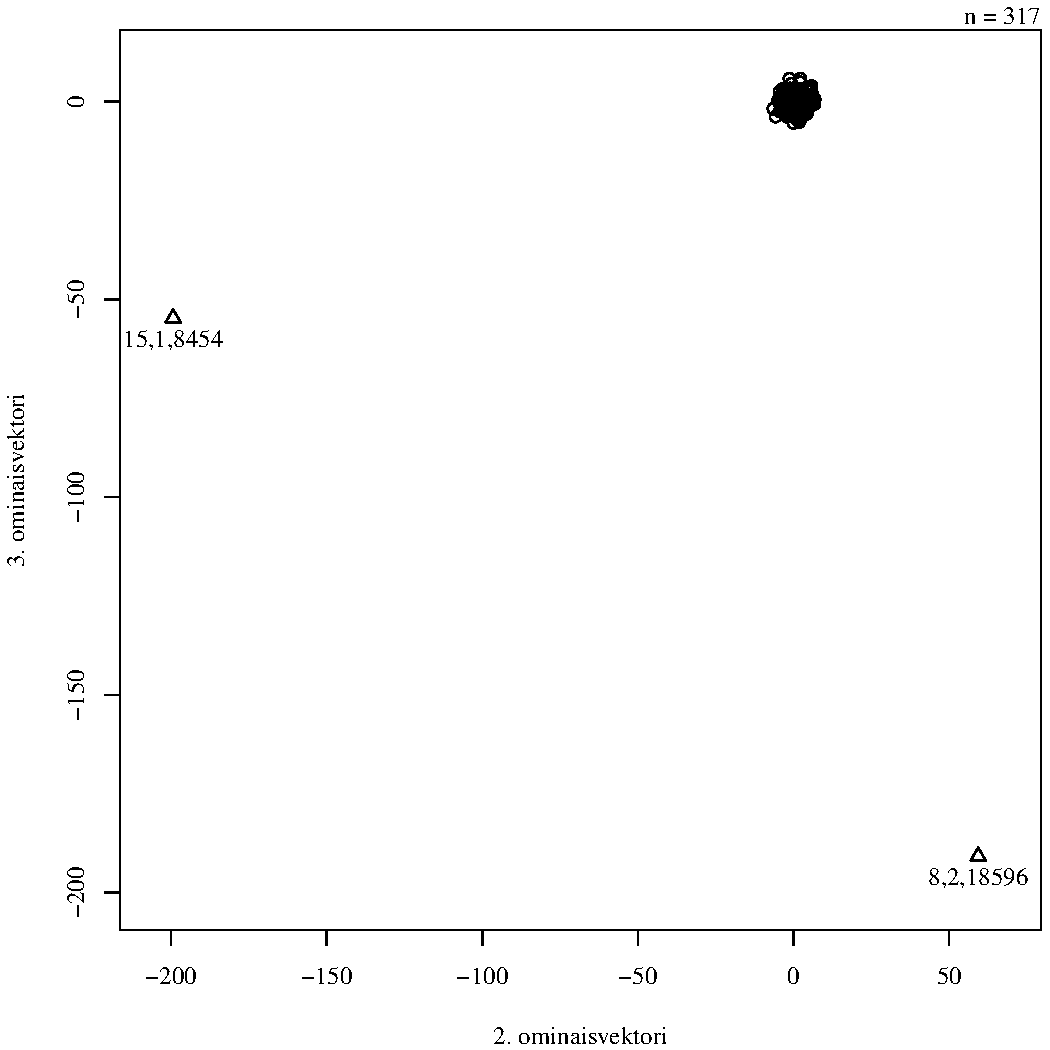
\includegraphics[width=11cm]{pics/diffuusiokuvat/service_882.pdf}
\caption{Resurssin 882 täristetty diffuusiokartta.}
\label{diffusio_882}
\end{figure}

\begin{figure}[p]
\centering
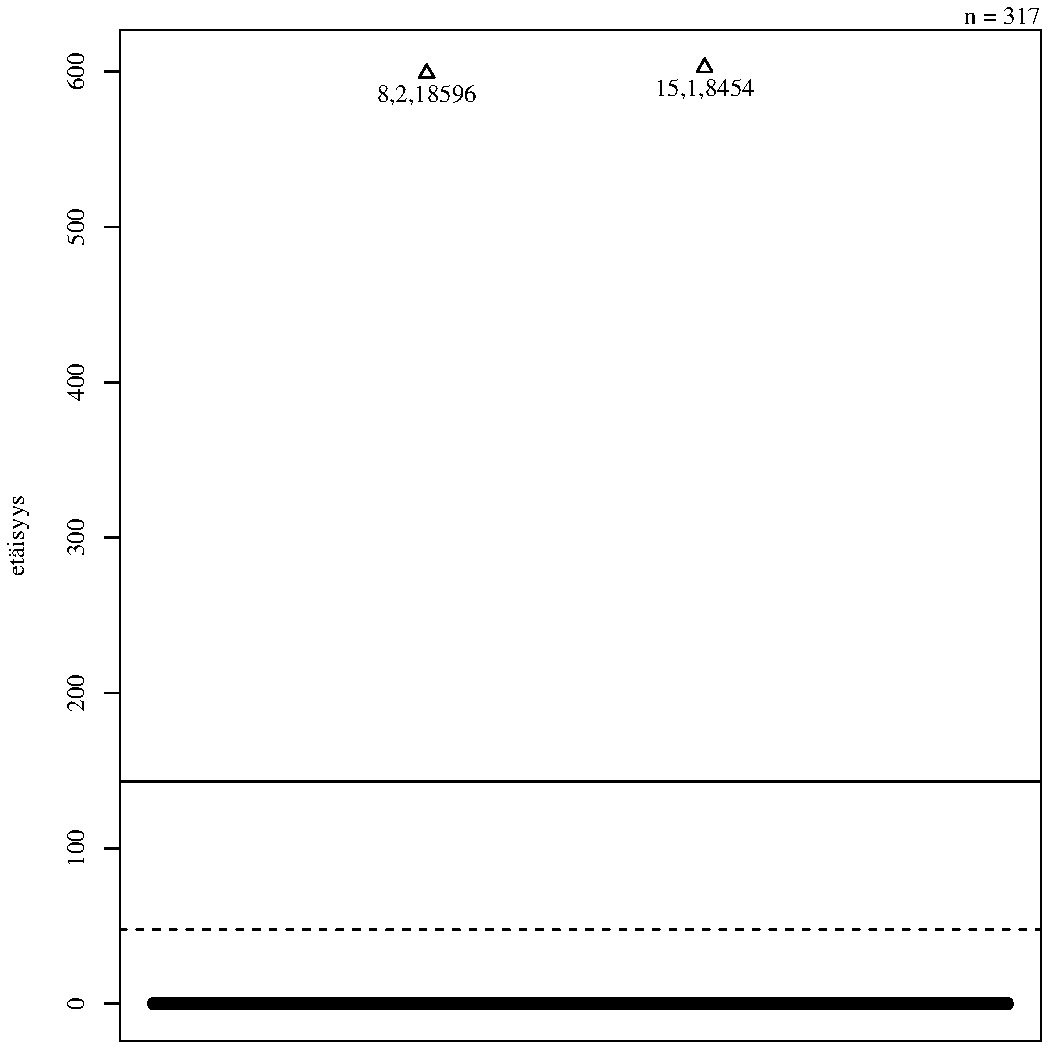
\includegraphics[width=11cm]{pics/tiheyskuvat/service_882.pdf}
\caption{Resurssin 882 poikkeavuuyskartta.}
\label{service_882}
\end{figure}

\section{Johtopäätöksiä ja kehitysideoita}

Analyysissä tuli hyvin esille se, että suurin osa liikenteestä oli hyvin samankaltaista. Tutkittavan materiaalin osalta tätä osattiin odottaa, mutta erilaisten pyyntöjen pieni määrä yllätti
siitä huolimatta. Ja vaikka kyseisestä otannasta ei varsinaisia tietoturvahyökäyksiä löydetty, olimme tyytyväisiä saatuihin tuloksiin. Tulokset osoittivat selkeästi sen, että esikäsittelijä toimi halutulla tavalla ja 
valittujen menetelmien avulla poikkeavat pyynnöt pystyttiin paikallistamaan. Myös todennäköisyys siihen, että analysoitavalle jaksolle olisi osunut jonkinlaisia tietoturvahyökkäyksiä, oli häviävän pieni
johtuen tiedon suuresta massasta. Kyseiset palvelut eivät muutenkaan olleet sellaisia, joihin hyökkääjillä olisi ollut suurta mielenkiintoa.  

Vaikka tässä työssä diffuusiokuvausten luomiseen käytettävien kyselyiden määrä rajoitti jonkin verran analyysin tekemistä, ei tämä käytännön ratkaisuissa muodostuisi ongelmaksi. Reaaliaikaisessa toteutuksessa
järjestelmälle opetetaan etukäteen normaali käyttäytyminen diffuusiokuvauksen avulla, jonka jälkeen uusien pisteiden paikka vertailujoukossa lasketaan yksitellen. Tällöin algoritmin käyttämä laskenta-aika
pysyy vakiona. Uudet pisteet voidaan projisoida diffuusiokuvaukseen esimerkiksi Nyströmin laajennuksen avulla, mutta tätä emme tähän työhön ottaneet enää mukaan. Menetelmä on kuitenkin hyvin tunnettu,
ja sitä on sovellettu monissa diffuusiokuvausten käyttöön pohjautuvissa tutkimuksissa.  

Seuraava looginen askel testauksissa olisi analysoida materiaalia rajatummalta alustalta ja lyhyemmältä ajanjaksolta. Esimerkiksi lokitiedot sellaisilta ajan hetkiltä, jolloin tietomurtoyritysten tiedetään tapahtuneen,
tarjoaisi erinomaiset puitteet testata tässä työssä käytettyjä ratkaisuja. Tätä kautta voitaisiin myös määrittää uusia parametreja, ja laajentaa käytettyjä menetelmiä. N-grammien lisäksi järjestelmä
voisi käyttää parametreina esimerkiksi samasta osoitteesta tulevien kyselyiden tiheyttä ja resurssipyynnöissä esiintyvien merkkien yleistä jakautumista. Käyttäjän IP-osoitteesta voitaisiin myös selvittää esimerkiksi
palveluntarjoaja, jonka kautta kysely tuli. Opetusjakson tarkempi määrittely tarjoaisi myös analyysin kannalta luotettavampaa tietoa. 

- Verkkokerroksen hyökkäykset jää huomaamatta. 

% -*- mode: LaTeX; coding: utf-8; -*-

\chapter{Yhteenveto}

TODO.


\bibliography{lahteet}{}
%\bibliographystyle{finplain}
\bibliographystyle{ieeetr}

\appendix

%\chapter{Published article}
%
%\includepdf[pages=-]{published_article.pdf}

\end{document}
